%%%%%%%%%%%%%%
%% Run LaTeX on this file several times to get Table of Contents,
%% cross-references, and citations.

%% If you have font problems, you may edit the w-bookps.sty file
%% to customize the font names to match those on your system.

%% w-bksamp.tex. Current Version: Feb 16, 2012
%%%%%%%%%%%%%%%%%%%%%%%%%%%%%%%%%%%%%%%%%%%%%%%%%%%%%%%%%%%%%%%%
%
%  Sample file for
%  Wiley Book Style, Design No.: SD 001B, 7x10
%  Wiley Book Style, Design No.: SD 004B, 6x9
%
%
%  Prepared by Amy Hendrickson, TeXnology Inc.
%  http://www.texnology.com
%%%%%%%%%%%%%%%%%%%%%%%%%%%%%%%%%%%%%%%%%%%%%%%%%%%%%%%%%%%%%%%%

%%%%%%%%%%%%%
% 7x10
%\documentclass{wileySev}

% 6x9
\documentclass{wileySix}

\usepackage{graphicx}
\usepackage{listings}
\usepackage{float}
\usepackage{hyperref}

\usepackage{color}
 
\definecolor{codegreen}{rgb}{0,0.6,0}
\definecolor{codegray}{rgb}{0.5,0.5,0.5}
\definecolor{codepurple}{rgb}{0.58,0,0.82}
\definecolor{backcolour}{rgb}{0.95,0.95,0.92}
 
\lstdefinestyle{mystyle}{
    backgroundcolor=\color{backcolour},   
    commentstyle=\color{codegreen},
    keywordstyle=\color{magenta},
    numberstyle=\tiny\color{codegray},
    stringstyle=\color{codepurple},
    basicstyle=\footnotesize,
    breakatwhitespace=false,         
    breaklines=true,                 
    captionpos=b,                    
    keepspaces=true,                 
    numbers=left,                    
    numbersep=5pt,                  
    showspaces=false,                
    showstringspaces=false,
    showtabs=false,                  
    tabsize=2,
    language=sh
}
 
\lstset{style=mystyle}

%%%%%%%
%% for times math: However, this package disables bold math (!)
%% \mathbf{x} will still work, but you will not have bold math
%% in section heads or chapter titles. If you don't use math
%% in those environments, mathptmx might be a good choice.

% \usepackage{mathptmx}

% For PostScript text
\usepackage{w-bookps}

%%%%%%%%%%%%%%%%%%%%%%%%%%%%%%%%%%%%%%%%%%%%%%%%%%%%%%%%%%%%%%%%
%% Other packages you might want to use:

% for chapter bibliography made with BibTeX
% \usepackage{chapterbib}

% for multiple indices
% \usepackage{multind}

% for answers to problems
% \usepackage{answers}

%%%%%%%%%%%%%%%%%%%%%%%%%%%%%%
%% Change options here if you want:
%%
%% How many levels of section head would you like numbered?
%% 0= no section numbers, 1= section, 2= subsection, 3= subsubsection
%%==>>
\setcounter{secnumdepth}{3}

%% How many levels of section head would you like to appear in the
%% Table of Contents?
%% 0= chapter titles, 1= section titles, 2= subsection titles, 
%% 3= subsubsection titles.
%%==>>
\setcounter{tocdepth}{2}

%% Cropmarks? good for final page makeup
%% \docropmarks

%%%%%%%%%%%%%%%%%%%%%%%%%%%%%%
%
% DRAFT
%
% Uncomment to get double spacing between lines, current date and time
% printed at bottom of page.
% \draft
% (If you want to keep tables from becoming double spaced also uncomment
% this):
% \renewcommand{\arraystretch}{0.6}
%%%%%%%%%%%%%%%%%%%%%%%%%%%%%%

%%%%%%% Demo of section head containing sample macro:
%% To get a macro to expand correctly in a section head, with upper and
%% lower case math, put the definition and set the box 
%% before \begin{document}, so that when it appears in the 
%% table of contents it will also work:

\newcommand{\VT}[1]{\ensuremath{{V_{T#1}}}}

%% use a box to expand the macro before we put it into the section head:

\newbox\sectsavebox
\setbox\sectsavebox=\hbox{\boldmath\VT{xyz}}

%%%%%%%%%%%%%%%%% End Demo


\begin{document}


\booktitle{Voice Cloning}
\subtitle{Clone Your Voice in 5 Seconds}

\author{Dinda Majesty\\
\affil{Politeknik Pos Indonesia}
%Floyd J. Fowler, Jr.\\
%\affil{University of New Mexico}
}

\offprintinfo{Voice Cloning, First Edition}{Dinda Majesty}

%% Can use \\ if title, and edition are too wide, ie,
%% \offprintinfo{Survey Methodology,\\ Second Edition}{Robert M. Groves}

%%%%%%%%%%%%%%%%%%%%%%%%%%%%%%
%% 
\halftitlepage

\titlepage


\begin{copyrightpage}{2021}
\end{copyrightpage}

\dedication{`Jika Kamu tidak dapat menahan lelahnya belajar, 
Maka kamu harus sanggup menahan perihnya Kebodohan.'
~Imam Syafi'i~}

\begin{contributors}
\name{Dinda Majesty,} Informatics Research Center., Politeknik Pos Indonesia, Bandung,
Indonesia
\name{Rolly Maulana Awangga,} Informatics Research Center., Politeknik Pos Indonesia, Bandung,
Indonesia
\name{Mohamad Nurkamal Fauzan,} Informatics Research Center., Politeknik Pos Indonesia, Bandung,
Indonesia
\name{Muhammad Yusril Helmi Setyawan,} Informatics Research Center., Politeknik Pos Indonesia, Bandung,
Indonesia

\end{contributors}

\contentsinbrief
\tableofcontents
\listoffigures
\listoftables
\lstlistoflistings


\begin{foreword}
Sepatah kata dari Kaprodi, Kabag Kemahasiswaan dan Mahasiswa
\end{foreword}

\begin{preface}
Buku ini berisi penjelasan teknologi serta tata cara yang harus dilakukan dalam pembuatan \textit{voice cloning} berbahasa indonesia. Buku ini diharapkan dapat membantu orang-orang memahami teknologi terkini terkait \textit{voice cloning} dan cara kerjanya, hal yang dibutuhkan dalam pembuatan \textit{voice cloning} serta cara membuat voice cloning.

\prefaceauthor{Tim Penulis}
\where{Bandung, Jawa Barat\\
Desember, 2022}
\end{preface}


\begin{acknowledgments}
Terima kasih atas semua masukan dari para dosen D4 Teknik Informatika Politeknik Pos Indonesia agar bisa membuat buku ini 
lebih baik dan lebih mudah dimengerti.

Terima kasih ini juga ditujukan khusus untuk dosen pembimbing yang 
telah membimbing dan membantu saya menyelesaikan pembuatan buku ini sebagai syarat kelulusan Internship.
\authorinitials{D. M.}
\end{acknowledgments}

\begin{acronyms}
\acro{ACGIH}{American Conference of Governmental Industrial Hygienists}
\acro{AEC}{Atomic Energy Commission}
\acro{OSHA}{Occupational Health and Safety Commission}
\acro{SAMA}{Scientific Apparatus Makers Association}
\end{acronyms}

\begin{glossary}
\term{Text to Speech}Merupakan proses pembuatan suara melalui inputan berupa text.

\term{Speech Synthesis}Merupakan kemampuan berbicara buatan (artificial) yang mirip seperti manusia.

\term{Voice Cloning}Merupakan sistem yang mampu menghasilkan suara tiruan yang memiliki kealamian dan kemiripan ucapan dengan sampel.

\term{Seq2Seq}Merupakan arsitektur jaringan saraf berulang yang biasa digunakan untuk memecahkan masalah bahasa yang kompleks.

\term{Tacotron-2}Merupakan arsitektur rancangan Google untuk menghasilkan mel-spectrogram yang digunakan dalam pembuatan audio.

\term{WaveNet}Merupakan model yang dapat menghasilkan audio berdasarkan mel-spectrogram.
\end{glossary}

\begin{symbols}
\term{A}Amplitude

\term{\hbox{\&}}Propositional logic symbol 

\term{a}Filter Coefficient

\bigskip

\term{\mathcal{B}}Number of Beats
\end{symbols}

\begin{introduction}

%% optional, but if you want to list author:

\introauthor{Dinda Majesty \\ Rolly Maulana Awangga\\ Mohamad Nurkamal Fauzan}
{Informatics Research Center, Politeknik Pos Indonesia\\
Bandung, Jawa Barat, Indonesia}
Perkembangan teknologi yang semakin maju dalam sistem \textit{Text to Speech (TTS)}  memungkinkan manusia membuat kloningan suara hanya dengan beberapa detik sampel suara. Hasil kloningan suara dapat dimodifikasi sesuai dengan inputan teks, sehingga kloningan suara tersebut akan mengucapkan kalimat yang sesuai dengan teks yang diinputkan. Suara yang dihasilkanpun terdengar alami mirip seperti suara manusia aslinya.
\end{introduction}

%%%%%%%%%%%%%%%%%%Isi Buku_
\chapter{Sistem Text to Speech (TTS)}
Sebelum mengetahui teknologi apa saja yang digunakan serta tata cara pembuatan sistem voice cloning ini, akan lebih baik apabila kita memahami terlebih dahulu mengenai sistem \textit{Text to Speech (TTS)}.

\section{Text to Speech (TTS)}
Text to Speech merupakan proses pembuatan suara melalui inputan berupa text\cite{DBLP:journals/corr/ArikDGMPPRZ17}. mungkin teman-teman bingung, bagaimana bisa text berubah menjadi suara, sementara text itu hanya dapat kita lihat menggunakan panca indra kita yaitu mata sedangkan suara merupakan sesuatu yang tidak bisa kita lihat menggunakan mata tetapi bisa kita dengar menggunakan telingga. Text to Speech ini ada untuk menjawab kebingungan teman-teman tersebut. Di zaman sekarang ini, dimana teknologi sudah semakin canggih, mengubah teks menjadi suara bukanlah hal yang sulit untuk dilakukan, apalagi setelah teman-teman mengenal deep learning, machine learning, dan artificial intelligence. Bagi teman-teman yang masih belum kenal, yuk kenalan dulu.
\begin{figure}[H]
        \centerline{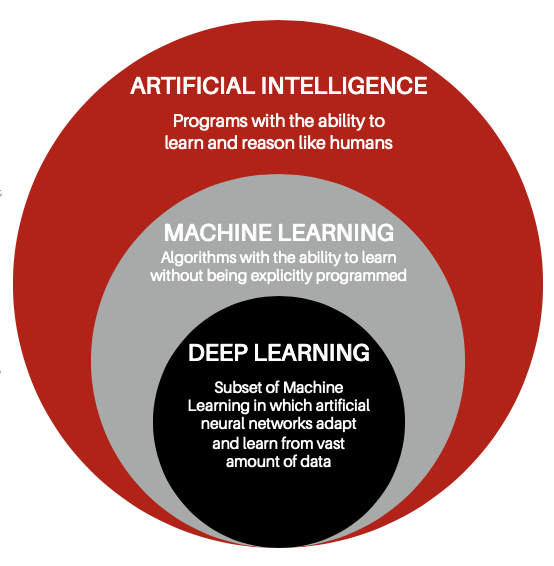
\includegraphics[scale=.75]{figures/korelasi}}
        \caption{Korelasi antara Deep Learning, Machine Learning, dan Artificial Intelligence}
		\label{korelasi}
\end{figure}

\subsection{Artificial Intelligence}
Artificial Intelligence (AI) merupakan kecerdasan yang dibuat dan diberikan atau diterapkan pada program komputer yang diharapkan memiliki kecerdasan seperti manusia sehingga memiliki kemampuan memahami, merencanakan, mengambil keputusan, dan problem solving. Dalam pembuatannya, setiap algoritma memungkinkan mesin untuk meniru, mengembangkan, dan berprilaku seperti manusia. Sederhananya AI itu merupakan sebuah teknologi yang memungkinkan kita menciptakan sebuah mesin yang memiliki kecerdasan berdasarkan pada perintah atau algoritma yang kita berikan pada program tersebut. algoritma berupa langkah-langkah yang kita lakukan dalam menyelesaikan suatu permasalahan. Misalnya kita ingin menciptakan mesin yang dapat menjawab semua pertanyaan kita seperti chatbot, maka kita membutuhkan algoritma atau langkah-langkah apa yang dilakukan oleh chatbot untuk memahami dan mampu memberikan respon secara cepat dan tepat kepada kita.

Artificial Intelligence dibuat dengan 3 tujuan, diantaranya:
\begin{enumerate}
\item tujuan utama, Membuat mesin menjadi lebih pintar dan terus mengalami peningkatan seiring dengan perkembangan teknologi
\item tujuan ilmiah, Memahami apa itu kecerdasan buatan sehingga dapat dimanfaatkan untuk membuat mesin yang lebih cerdas dalam membantu dan memecahkan masalah secara efektif dan efisien.
\item tujuan entrepreneurial, Membuat mesin lebih bermanfaat sehingga memudahkan manusia dalam melakukan perkerjaan dan memecahkan masalah secara cepat, tepat, dan lebih teliti.
\end{enumerate}

\subsection{Machine Learning}
Machine Learning (ML) merupakan bagian dari Artificial Intelligence yang ditambahkan dengan metode-metode statistika dengan tujuan agar mesin dapat meningkat-kan pengalamannya berdasarkan kepada data-data yang ada dan dilatih pada mesin tersebut. Dengan begitu mesin dapat melakukan tugas tertentu berdasarkan data dan algoritma yang diterapkan padanya. Data dan Algoritma yang dirancang membuat mesin terus mengalami peningkatan dari waktu ke waktu. Sebagai contoh, pada pembuatan sistem untuk memprediksi tweet yang bersifat positif, negatif, atau netral kita akan membutuhkan data tweet dari para pengguna twitter, kita bisa dapatkan melalui API yang telah disediakan oleh twitter. pada tahap pertama, kita mengambil 100 data tweet yang terdiri dari tweet positif, negatif, dan netral. Lalu kita melatih mesin menggunakan 100 data tersebut dan menggunakan algoritma naive bayes untuk mengetahui apakah data hasil prediksi kita sama dengan data tweet aslinya dan menghitung akurasi dari algoritma yang telah kita buat. Pada tahap pertama akurasi menunjukkan angkat 90\% dan ketika kita melakukan training kembali kepada algoritma atau model yang telah kita buat dengan menggunakan data yang lebih banyak lagi maka mesin akan menjadi lebih terlatih dan kemungkinan kesalahan prediksi menjadi sangat kecil bahkan akurasi yang didapatkan dari model bisa mencapai 99\% atau bahkan kita bisa mengganti algoritma yang kita gunakan menggunakan algoritma lainnya yang menghasilkan akurasi yang lebih baik dari model atau algoritma kita sebelumnya. hal inilah yang dimaksud dengan machine learning, ada data dan algorithma serta perhitungan-perhitungan yang sering kita jumpai dalam statistika seperti perhitungan akurasi, rata-rata (mean), median, recall, precision, dll.

\subsection{Deep Learning}
Setelah mengenal AI dan ML saatnya kita mengenal Deep Learning (DL) yang merupakan bagian dari Machine Learning yang berkaitan dengan algoritma yang berdasarkan pada struktur dan fungsi otak atau sering dikenal sebagai jaringan saraf tiruan. Pada dasarnya Deep Learning memiliki konsep seperti Machine Learning hanya saja dalam konteks yang lebih dalam. Contohnya, pada deep learning kita ingin membuat mesin dapat mengetahui apakah hewan yang ada digambar merupakan seekor anjing atau kucing, maka kita akan membuat algoritma untuk melakukan pengecekan seperti melakukan pengecekan pada bentuk ekor, bentuk telinga, apakah memiliki kumis atau tidak, dan ciri-ciri lainnya yang membuat kucing dan anjing terlihat berbeda tanpa kita perlu memberikan fitur pembedanya atau fitur mana yang lebih penting untuk dapat mengidentifikasi hewan tersebut secara manual. Deep Learning dapat mengetahui fitur tersebut tanpa kita beritahu secara manual seperti pada Machine Learning seperti terlihat pada gambar \ref{deep learning}. Oleh karena itu Deep Learning dianggap sebagai otak utama yang menciptakan kecerdasan buatan yang lebih manusiawi.
\begin{figure}[H]
        \centerline{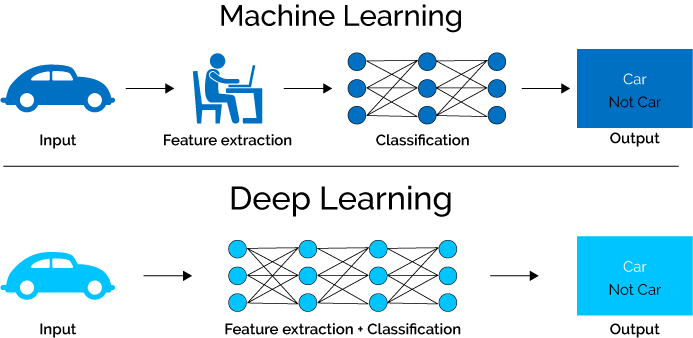
\includegraphics[scale=.45]{figures/deeplearning}}
        \caption{Perbedaan Machine Learning dan Deep Learning}
		\label{deep learning}
\end{figure}

Text to Speech termasuk bagian dari Deep Learning lebih tepatnya Neural Network\cite{li2017deep}. Neural Network merupakan cabang ilmu yang mengadopsi cara berpikir dan cara bekerja otak manusia yang memberikan rangsangan/stimulus (input), melalukan proses, dan menghasilkan sesuatu (output). Output dihasilkan dari inputan yang diberikan dan proses yang dilakukan oleh otak manusia. Kemampuan otak untuk memproses inputan atau informasi ini yang akan membuat otak manusia selalu mempelajari hal-hal baru dan terus berkembang, begitupun dengan mesin yang diberikan kecerdasan buatan atau AI. Contohnya saja ketika kita berusia 5 tahun dan otak kita belum memahami informasi-informasi yang sulit seperti pelajaran matematika dasar, menambah dan mengurangi ataupun membagi dan mengalikan angka. Setelah kita mempelajarinya selama 6 tahun di Sekolah Dasar maka otak kita sekarang bisa memahaminya bahkan hal tersebut merupakan hal yang sangat gampang. Pada dasarnya konsep AI sama dengan otak manusia yang selalu berkembang dan mempelajari hal-hal yang baru berdasarkan inputan atau informasi apa yang diberikan kepada otak dan otak akan memproses inputan tersebut hingga dapat memahami dan mengeluarkan hasil dari proses tersebut (output).
Dalam pembuatan voice cloning ini kita akan mengajarkan kepada mesin cara membaca text dan mengucapkannya dengan menggunakan suara seperti yang kita contohkan, Oleh karena itu kita membutuhkan sistem text to speech.


\section{Cara Kerja TTS}
Cara kerja TTS terdiri dari 2 proses, dapat dilihat pada gambar \ref{cara kerja}:
\begin{enumerate}
\item Model Teks ke Spektogram, model ini mengubah teks menjadi fitur yang selaras dengan waktu seperti spektogram, mel-spektogram, atau frekuensi F0 dan fitur linguistik lainnya. ada beberapa model yang bisa digunakan untuk mengubah teks menjadi spektogram, diantaranya yaitu Tacotron, Tacotron2, Deep Voice 3, dll. Model ini juga disebut sebagai model encoder-decoder.
\item Model spektogram ke audio, model ini akan mengonversi spektogram yang dihasilkan menjadi audio. Model ini disebut sebagai vocoder. beberapa model yang banyak digunakan untuk membuat vocoder yaitu WaveGlow, Griffin-Lim Algorithm, WaveNet, dll.
Model Tacotron-2 sebagai model encoder-decoder dan model WaveNet yang dimodifikasi sebagai vocoder akan dibahas secara mendalam pada buku ini.
\end{enumerate}
\begin{figure}[H]
        \centerline{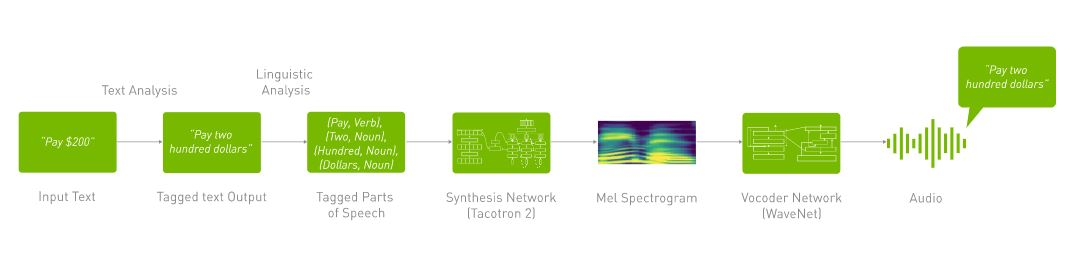
\includegraphics[scale=.40]{figures/cara_kerja_tts}}
        \caption{Cara Kerja Text to Speech (TTS)}
		\label{cara kerja}
\end{figure}


\chapter{Neural Network}
\section{Neural Network}
Neural Network terinspirasi dari cara kerja neuron yang ada pada otak manusia, neuron bertugas sebagai penerima stimulus/rangsangan dan pengirim informasi yang akan diolah atau diproses oleh otak menjadi suatu output. Neuron merupakan sistem saraf pusat dan terdapat sekitar 100 miliar neuron yang ada pada tubuh manusia. Perhatikan gambar \ref{neuron}
\begin{figure}[H]
        \centerline{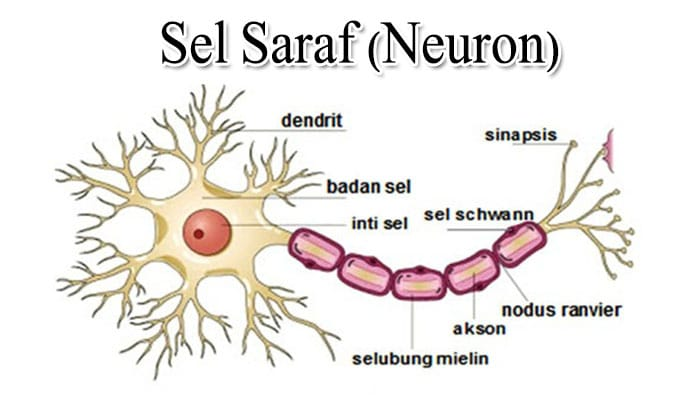
\includegraphics[scale=.45]{figures/neuron}}
        \caption{Sel Saraf (Neuron)}
		\label{neuron}
\end{figure}

Neuron terdiri dari 3 bagian yaitu akson (akar), soma (batang), dan dendrite (cabang). Neuron juga dibedakan menjadi 3 yaitu neuron sensorik atau sel saraf indra karena fungsinya yang berhubungan dengan penerima (indra) dan saraf pusat (otak dan sumsum tulang belakang). Neuron motorik atau sel saraf penggerak yang berfungsi membawa rangsangan dari saraf pusat (otak dan sumsum tulang belakang) ke otot. Terakhir yaitu neuron asosiasi ataus sel saraf penghubung, sel ini menghubung-kan atau meneruskan rangsangan dari sel saraf sensorik ke sel saraf motorik.

Tiap neuron yang ada dalam otak kita saling terhubung dan berkirim informasi atau rangsangan berupa neurotransmitter, neuron yang saling berinteraksi dengan mengirimkan rangsangan ini akan menghasilkan kemampuan tertentu pada kerja otak kita. Contohnya, ketika kita bertemu dengan seorang kenalan yang menyapa kita maka otak akan berkerja sehingga dapat mengenali orang tersebut dan akan menghasilkan respon atau output, outputnya bisa berupa sapaan, lambaian tangan, obrolan, dan hal-hal lainnya yang biasa kita lakukan apabila bertemu dengan seseorang yang kita kenal. Jadi secara ilmiahnya, inputan atau rangsangan yang diterima yaitu berupa sapaan dari orang yang dikenali. Rangsangan ini akan diterima oleh alat indra (mata, telinga, hidung, lidah, dan kulit) melalui sel reseptor, kemudian akan diteruskan dalam bentuk impuls berupa arus listrik yang diteruskan ke sel saraf sensorik melalui sinapsis, lalu melewati sel saraf konektor menuju otak. Pada otak informasi akan diolah terlebi dahulu kemudian dikirimkan ke sel saraf motorik dan memberikan atau menghasilkan reaksi berupa sapaan, gerakan berupa lambaian tangan dll. Inilah proses kerja otak manusia begitupun dengan neural network yang terinspirasi dari cara neuron bekerja pada otak manusia. Siapa sangka mesin yang merupakan benda mati akan bisa berprilaku dan berkerja seperti layaknya manusia. Hingga saat ini sangat banyak diminati dan terus dikembangkan dengan tujuan dapat membantu memudahkan manusia dalam bekerja.

\subsection{Sejarah Neural Network}
\begin{figure}[H]
        \centerline{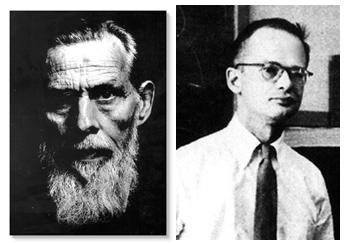
\includegraphics[scale=1]{figures/nn1}}
        \caption{McCulloch dan Pitts, penemu pertama Neural Network}
		\label{penemu}
\end{figure}
Neural Network bermula ketika Warren McMulloch yang merupakan seorang neurofisiologi dan Walter Pitts yang merupakan seorang ahli matematika menulis makalah tentang cara kerja dari neuron pada tahun 1943. Kemudian diperkuatnya konsep neuron dalam buku yang ditulis oleh Donald Hebb pada tahun 1949 yang berjudul The Organization of Behavior yang menunjukkan bahwa jaringan syaraf akan bertambah kuat setiap kali digunakan. Kemudian dilanjutkan dengan penelitian di IBM untuk mensimulasikan neural network tahun 1950 yang dipimpin oleh Nathanial Rochester.

Dengan diadakannya konferensi Dartmouth pada tahun 1956 yang membahas tentang penelitian neural network oleh John McCarthy memperkuat konsep mengenai neural network. Lalu pada tahun 1957, John Von Neumann menyarankan untuk meniru fungsi neuron menggunakan relay telegraf atau tabung vakum. Dengan adanya penemuan two-layer-network yang dikenal dengan percepton. Percepton berguna untuk menghitung jumlah input, mengurangi treshold, dan meneruskan salah satu dari dua nilai yang mungkin keluar sebagai hasil, penemuan ini ditemukan oleh Frank Rosenblatt pada tahun 1958. 

Pada tahun 1959, diperkenalkan model neural network pertama yang dikenal dengan ADALINE (Adaptive Linear Elements) dan MEDALINE (Multiple Adaptive Linear Elements). Model ini merupakan model pertama yang diterapkan pada permasalahan yang ada di dunia nyata. Model ini berfungsi untuk menghilangkan gema pada saluran telepon. Pengembangan model ini dilakukan oleh Bernard Widrow dan Marcian Hoff dari Stanford.

Pada tahun 1982 dalam makalah yang dipresentasikan pada National Academy of Sciences tentang pendekatan untuk menciptakan perangkat yang berguna, menyenangkan, pandai berbicara dan kharismatik, makalah ini dipresentasikan oleh John Hopfield. Lalu konferensi International Institute of Electrical and Electronics (IEEE) mengadakan konferensi mengenai Neural Network yang dihadiri oleh lebih dari 1.800 peserta pada tahun 1987. Sekarang, Neural Network telah diterapkan pada classification, approximation, prediction, recognition, memory simulation, clusterization, dll. 

\subsection{Struktur Neuron Pada Otak Manusia}
Ide dasar dari pembuatan Neural Network dimulai dari cara kerja otak manusia dalam belajar dan struktur otak manusia yang terdiri dari neuron yang saling terhubung, mengirim, dan menerima informasi. Satu neuron memiliki satu akson dan minimal satu dendrit. Setiap sel saraf terhubung dengan sel saraf lain yang saling berinteraksi dan menghasilkan kemampuan tertentu pada kerja otak manusia sehingga otak menjadi semakin pintar atau memiliki banyak kemampuan serta pengetahuan. Misalnya kemampuan otak ketika kita masih kecil dengan kemampuan otak kita saat dewasa tidak akan sama, karena otak kita selalu belajar hingga kita dapat memahami hal-hal yang baru dan kemampuan otak kita semakin berkembang.

Perhatikan gambar \ref{neuron}, pada gambar neuron terdiri dari:

\begin{enumerate}
\item Dendrit (Dendrites) berfungsi untuk mengirimkan impuls yang diterima berupa arus listrik ke badan sel saraf.
\item Akson (Axon) berfungsi untuk mengirimkan impuls dari badan sel ke jaringan lain.
\item Sinapsis berfungsi sebagai unit fungsional (penghubung) di antara dua sel saraf.
\item Selubung mielin sebagai pelindung akson dan pemberi nutrisi.
\item Nodus Ranvier berfungsi untuk mempercepat impuls saraf.
\item Nukleus merupakan inti sel yang bertugas sebagai pengatur kegiatan sel saraf (neuron).
\item Soma berfungsi untuk mengendalikan metabolisme keseluruhan dari neuron.
\item Sel Schwann adalah penunjang sel saraf berupa lemak yang berfungsi menghasilkan mielin atau selubung saraf.
\end{enumerate}

Berikut cara kerja otak manusia:

Ketika Sebuah neuron menerima impuls dari neuron lain melalui dendrit, maka dendrit akan mengirimkan sinyal tersebut ke badan sel saraf. Selanjutnya Akson akan menerima sinyal dari badan sel dan mengirimkannya ke sel saraf lain. Akson dari sel saraf ini bercabang-cabang, akson sel saraf satu berhubungan dengan akson sel saraf dua melalui sinapsis. Sinapsis adalah unit fungsional antara 2 buah sel saraf, misal sel A dan sel B, akson sel A akan berhubungan dengan dendrit sel B melalui sinapsis. Kekuatan sinapsis bisa menurun/meningkat tergantung tingkat propagasi sinyal yang diterimanya. Impuls-impuls sinyal (informasi) akan diterima oleh neuron lain jika memenuhi batasan tertentu, dikenal dengan nilai ambang (threshold).

\subsection{Struktur Neural Network}
Dari struktur neuron pada otak manusia, dan proses kerja yang dijelaskan di atas, maka konsep dasar pembangunan neural network buatan (Artificial Neural Network) terbentuk. Ide mendasar dari Artificial Neural Network (ANN) adalah mengadopsi mekanisme berpikir sebuah sistem atau aplikasi yang menyerupai otak manusia, baik untuk pemrosesan berbagai sinyal elemen yang diterima, toleransi terhadap kesalahan/error, dan juga parallel processing.

Karakteristik dari ANN dilihat dari pola hubungan antar neuron, metode penentuan bobot dari tiap koneksi, dan fungsi aktivasinya. Gambar di atas menjelaskan struktur ANN secara mendasar, yang dalam kenyataannya tidak hanya sederhana seperti itu.

Input, berfungsi seperti dendrite
Output, berfungsi seperti akson
Fungsi aktivasi, berfungsi seperti sinapsis
Neural network dibangun dari banyak node/unit yang dihubungkan oleh link secara langsung. Link dari unit yang satu ke unit yang lainnya digunakan untuk melakukan propagasi aktivasi dari unit pertama ke unit selanjutnya. Setiap link memiliki bobot numerik. Bobot ini menentukan kekuatan serta penanda dari sebuah konektivitas.

Proses pada ANN dimulai dari input yang diterima oleh neuron beserta dengan nilai bobot dari tiap-tiap input yang ada. Setelah masuk ke dalam neuron, nilai input yang ada akan dijumlahkan oleh suatu fungsi perambatan (summing function), yang bisa dilihat seperti pada di gambar dengan lambang sigma. Hasil penjumlahan akan diproses oleh fungsi aktivasi setiap neuron, disini akan dibandingkan hasil penjumlahan dengan threshold (nilai ambang) tertentu. Jika nilai melebihi threshold, maka aktivasi neuron akan dibatalkan, sebaliknya, jika masih dibawah nilai threshold, neuron akan diaktifkan. Setelah aktif, neuron akan mengirimkan nilai output melalui bobot-bobot outputnya ke semua neuron yang berhubungan dengannya. Proses ini akan terus berulang pada input-input selanjutnya.

ANN terdiri dari banyak neuron di dalamnya. Neuron-neuron ini akan dikelompokkan ke dalam beberapa layer. Neuron yang terdapat pada tiap layer dihubungkan dengan neuron pada layer lainnya. Hal ini tentunya tidak berlaku pada layer input dan output, tapi hanya layer yang berada di antaranya. Informasi yang diterima di layer input dilanjutkan ke layer-layer dalam ANN secara satu persatu hingga mencapai layer terakhir/layer output. Layer yang terletak di antara input dan output disebut sebagai hidden layer. Namun, tidak semua ANN memiliki hidden layer, ada juga yang hanya terdapat layer input dan output saja.

\subsection{Cara Kerja Neural Network}
Cara kerja Neural Network sama halnya dengan proses belajar yang dilakukan oleh otak manusia dengan menggunakan contoh atau disebut juga supervised learning. Neural network dikonfigurasikan pada aplikasi tertentu seperti pengklasifikasian data atau pengenalan pola. Neural Network memproses informasi seperti cara kerja otak manusia yang terdiri dari sejumlah besar elemen pemrosesan yang saling berhubungan dan berkerja secara paralel dalam menyelesaikan masalah. Neural Network dapat digunakan untuk memperoleh informasi atau pengetahuan dari data-data yang rumit, mengekstrak pola, mendeteksi tren yang memiliki kompleksitas yang rumit untuk dipelajari manusia ataupun teknik komputasi lainnya. Oleh karena itu, neural network yang telah dilatih hingga dapat menganalisis dan memproses informasi dari data dapat dikategorikan sebagai ahli. Neural Network sangat cocok untuk menyelesaikan beberapa masalah terkait prediksi yang membutuhkan pemahaman dan analisis yang baik contohnya prediksi pergerakan data time-series. Sedangkan algoritma komputer konvensional lebih cocok untuk menyelesaikan masalah terkait operasi aritmatika. Namun, pada beberapa masalah Neural Network dan Algoritma Komputer Konvensional dikombinasikan agar dapat memberikan kinerja maksimum.

\chapter{Sequence to Sequence (Seq2Seq)}
\section{Model Sequence to Sequence}
Model Sequence to Sequence (seq2seq) merupakan arsitektur Jaringan Saraf Berulang yang biasa digunakan untuk memecahkan masalah bahasa yang kompleks seperti Terjemahan, Menjawab Pertanyaan, membuat Chatbot, Peringkasan Teks, dll. Contoh penggunaan model seq2seq dapat dilihat pada gambar \ref{seqtoseq}
\begin{figure}[H]
        \centerline{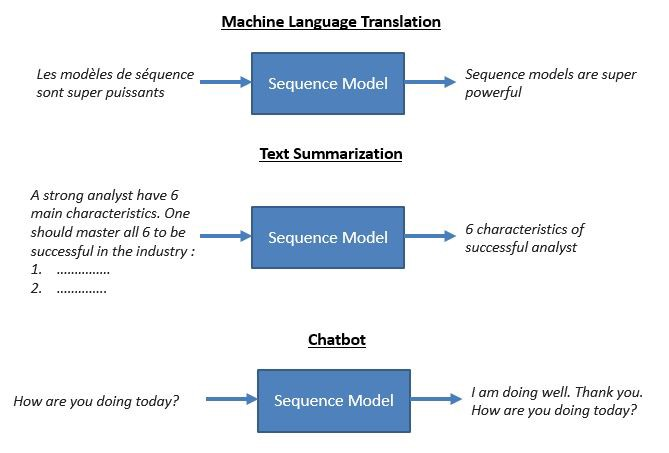
\includegraphics[scale=.45]{figures/sequence_model}}
        \caption{Contoh Penggunaan Model Sequence to Sequence}
		\label{seqtoseq}
\end{figure}

Model seq2seq sering dijumpai pada sistem yang sering kita gunakan sehari-hari. Model seq2seq mendukung aplikasi seperti Google Terjemahan, perangkat yang mendukung suara, voice assistant, chatbot, dll . Berikut ini adalah beberapa aplikasinya:

\begin{enumerate}
\item Google Translate, makalah tahun 2016 dari Google menunjukkan bagaimana kualitas terjemahan model seq2seq yang mendekati atau bahkan melampaui semua hasil yang dipublikasikan saat ini.
\begin{figure}[H]
        \centerline{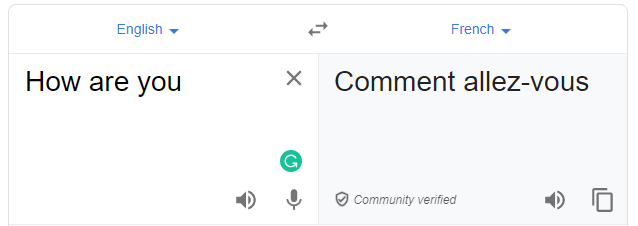
\includegraphics[scale=.5]{figures/terjemahan}}
        \caption{Google Translate}
		\label{terjemahan}
\end{figure}
\item Speech Recognition, makalah Google yang membandingkan model seq2seq yang ada pada pengenalan suara.
\begin{figure}[H]
        \centerline{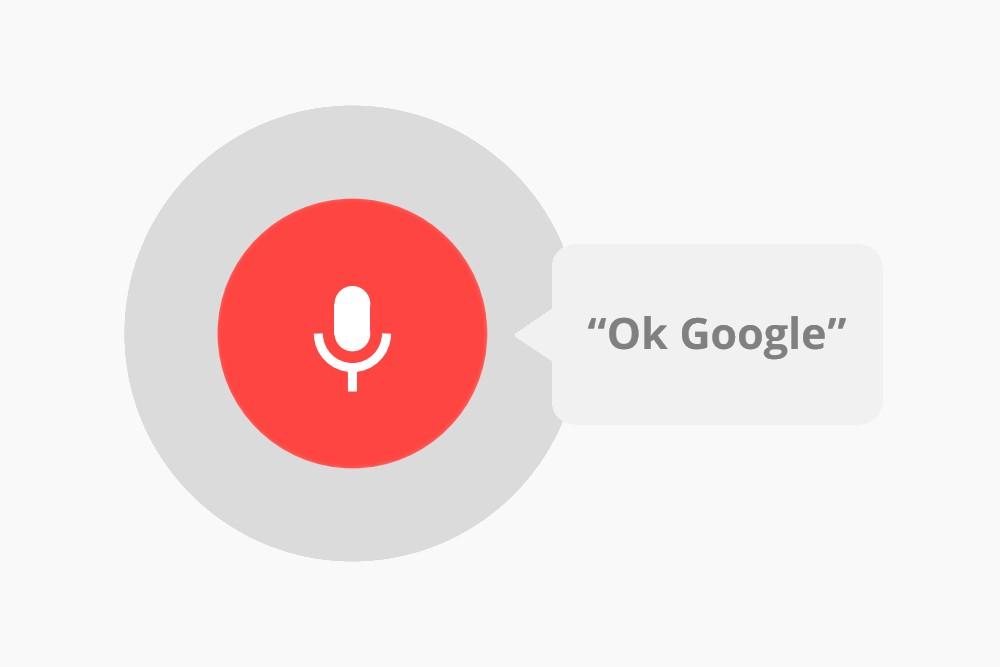
\includegraphics[scale=.25]{figures/voice}}
        \caption{Speech Recognition}
		\label{voice}
\end{figure}
\item Video Captioning –  Secara otomatis membuat subtitle video untuk setiap frame, termasuk deskripsi isyarat suara (seperti mesin yang dinyalakan, orang yang tertawa di latar belakang, dll.).
\begin{figure}[H]
        \centerline{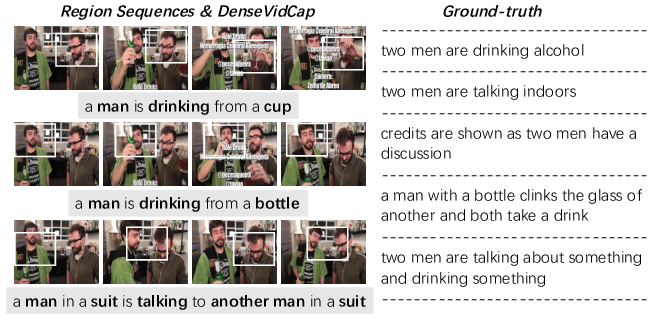
\includegraphics[scale=.45]{figures/video-captioning}}
        \caption{Video Captioning}
		\label{video}
\end{figure}
\end{enumerate}

Beberapa aplikasi tersebut membuat model seq2seq dipandang sebagai solusi terbaik. Model ini dapat digunakan sebagai solusi untuk setiap masalah berbasis urutan, terutama yang input dan outputnya memiliki ukuran dan kategori yang berbeda.

\subsection{Arsitektur Encoder-Decoder}
Arsitektur yang paling umum digunakan untuk membangun model Seq2Seq adalah arsitektur Encoder-Decoder.

Encoder:
\begin{enumerate}
\item Encoder dan decoder adalah model LSTM (atau terkadang model GRU)
\item Encoder membaca urutan input dan merangkum informasi dalam sesuatu yang disebut internal state vectors atau context vector (dalam kasus LSTM ini disebut hidden state dan cell state vectors). Kami membuang output encoder dan hanya mempertahankan status internal. Vektor konteks ini bertujuan untuk merangkum informasi untuk semua elemen input untuk membantu dekoder membuat prediksi yang akurat.
\item Hidden State h\_i dihitung menggunakan rumus pada gambar \ref{rumus}:
\begin{figure}[H]
        \centerline{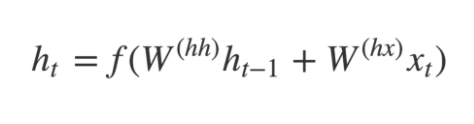
\includegraphics[scale=.3]{figures/rumus}}
        \caption{Rumus Hidden State}
		\label{rumus}
\end{figure}
\end{enumerate}

Perhatikan gambar \ref{encoder} LSTM membaca data dari satu urutan secara berurutan. Jadi jika inputnya adalah barisan dengan panjang 't', kita katakan bahwa LSTM membacanya dalam langkah waktu 't'.

\begin{figure}[H]
        \centerline{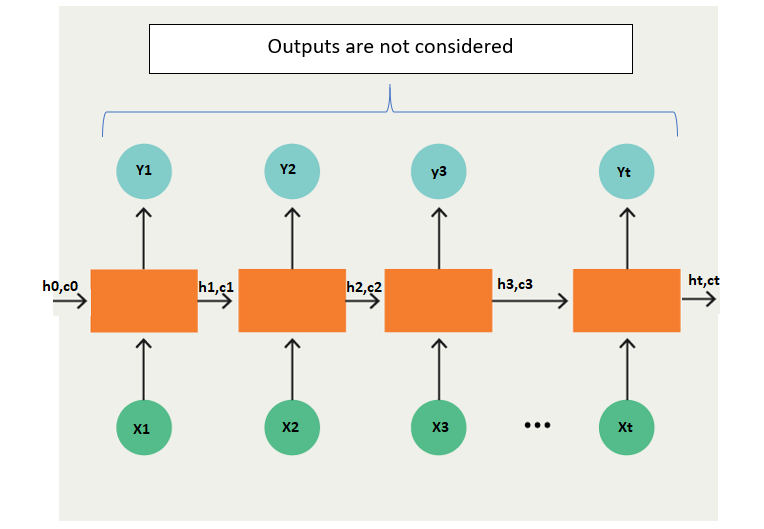
\includegraphics[scale=.45]{figures/lstm}}
        \caption{Encoder}
		\label{encoder}
\end{figure}

\begin{enumerate}
\item Xi = Urutan input pada langkah waktu i.
\item hi dan ci = LSTM mempertahankan dua status ('h' untuk status tersembunyi dan 'c' untuk status sel) pada setiap langkah waktu. h dan c yang dikombinasikan bersama-sama merupakan keadaan internal LSTM pada langkah waktu i.
\item Yi = Urutan keluaran pada langkah waktu i. Yi sebenarnya adalah distribusi probabilitas atas seluruh kosakata yang dihasilkan dengan menggunakan aktivasi softmax. Jadi setiap Yi adalah vektor dengan ukuran “vocab\_size” yang mewakili distribusi probabilitas.
\end{enumerate}

Dekoder:
\begin{enumerate}
\item Decoder adalah LSTM yang status awalnya diinisialisasi ke final state Encoder LSTM, yaitu context vector dari final cell encoder dimasukkan ke first cell pada jaringan decoder. Dengan menggunakan initial states ini, dekoder mulai menghasilkan output sequence, dan output ini juga dipertimbangkan untuk output selanjutnya.
\item Tumpukan beberapa unit LSTM di mana masing-masing memprediksi output y\_t pada langkah waktu t.
\item Setiap unit berulang menerima hidden state dari unit sebelumnya menghasilkan dan mengeluarkan hidden statenya sendiri.
\item Setiap hidden state h\_i dihitung menggunakan rumus:
\begin{figure}[H]
        \centerline{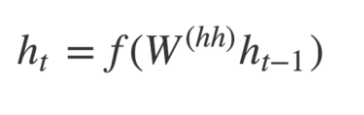
\includegraphics[scale=.3]{figures/rumus-encoder}}
        \caption{Rumus Hidden State}
		\label{rumus1}
\end{figure}
\item Output y\_t pada langkah waktu t dihitung dengan menggunakan rumus:
\begin{figure}[H]
        \centerline{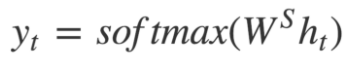
\includegraphics[scale=.3]{figures/rumus2}}
        \caption{Rumus Hidden State}
		\label{rumus2}
\end{figure}

Menghitung output dilakukan dengan menggunakan hidden state pada langkah waktu saat ini bersama-sama dengan respective weight W(S). Softmax digunakan untuk membuat vektor probabilitas yang akan membantu kita menentukan hasil akhir (misalnya kata dalam masalah tanya jawab).
\begin{figure}[H]
        \centerline{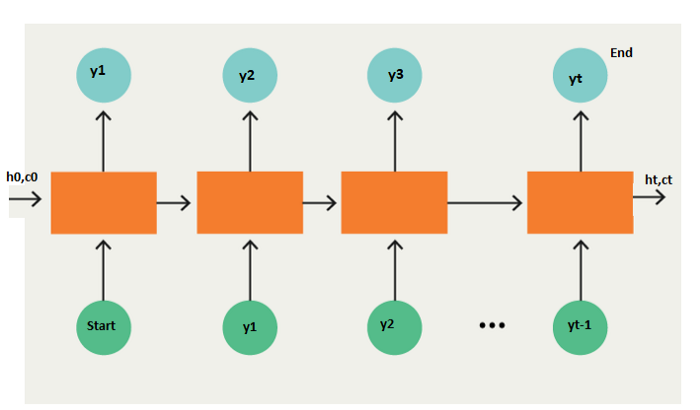
\includegraphics[scale=.45]{figures/lstm1}}
        \caption{Decoder}
		\label{decoder}
\end{figure}
\end{enumerate}

Sebagai contoh kita akan menambahkan dua token dalam urutan output sebagai berikut:

Contoh:
“ START\_ John pekerja keras \_END ”.

Poin yang paling penting adalah bahwa first state (h0, c0) dari dekoder diatur ke final state dari encoder. Ini secara intuitif berarti bahwa decoder dilatih untuk mulai menghasilkan urutan output tergantung pada informasi yang dikodekan oleh encoder. Sehingga loss dihitung pada output yang diprediksi dari setiap langkah waktu dan error disebarkan kembali melalui waktu untuk memperbarui parameter jaringan. Training network dalam jangka waktu yang lebih lama dengan jumlah data yang cukup besar menghasilkan prediksi yang cukup bagus.

\begin{figure}[H]
        \centerline{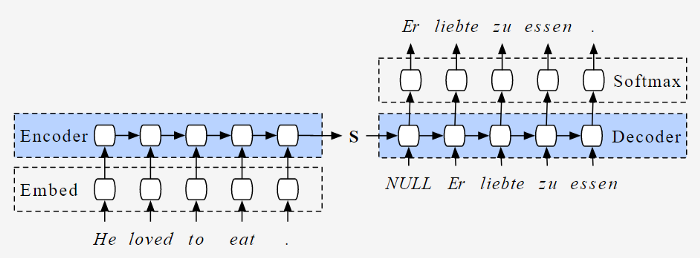
\includegraphics[scale=.45]{figures/arsitektur-encoder-decoder}}
        \caption{Arsitektur Encoder-Decoder Secara Keseluruhan}
		\label{endecoder}
\end{figure}

\begin{enumerate}
\item Selama inferensi dihasilkan satu kata pada satu waktu.
\item Initial state dekoder diatur ke final state encoder.
\item initial input ke dekoder selalu berupa token START.
\item Pada setiap time step kita harus mempertahankan status dekoder dan menetapkannya sebagai status awal untuk time step berikutnya.
\item Pada setiap time step, output yang diprediksi diumpankan sebagai input pada time step berikutnya.
\item loop akan dihentikan ketika decoder memprediksi token END.
\end{enumerate}

Sebuah sequence untuk model urutan memiliki dua bagian - encoder dan decoder.  Kedua bagian itu praktis adalah dua model jaringan saraf yang berbeda digabungkan menjadi satu jaringan raksasa. Secara umum, tugas jaringan encoder adalah memahami urutan input, dan membuat representasi dimensi yang lebih kecil darinya. Representasi ini kemudian diteruskan ke jaringan decoder yang menghasilkan urutannya sendiri yang mewakili output. Mari kita ambil contoh agen percakapan untuk memahami konsepnya.

\begin{figure}[H]
        \centerline{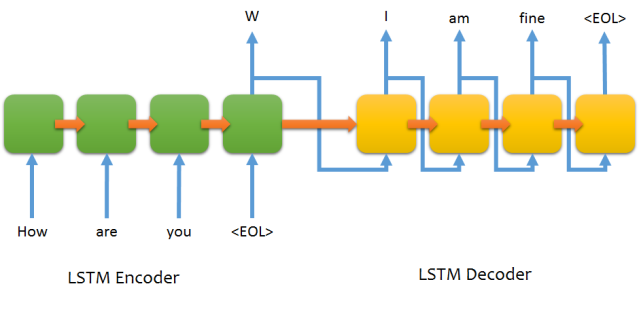
\includegraphics[scale=.65]{figures/chatbot}}
        \caption{Chatbot dengan Seq2Seq Model}
		\label{chatbot}
\end{figure}

Pada gambar \ref{chatbot}, urutan input adalah "Bagaimana kabarmu". Jadi ketika urutan input seperti itu dilewatkan melalui jaringan encoder-decoder yang terdiri dari blok LSTM (sejenis arsitektur RNN), decoder menghasilkan kata-kata satu per satu di setiap langkah waktu iterasi dekoder. Setelah satu iterasi penuh, urutan output yang dihasilkan adalah "Saya baik-baik saja".

\subsection{Kekurangan Model Encoder-Decoder}
Ada dua kelemahan utama arsitektur ini, keduanya terkait dengan panjang.

Pertama, seperti halnya manusia, arsitektur ini memiliki memori yang sangat terbatas. Keadaan tersembunyi terakhir dari LSTM, yang kami sebut S atau W , adalah saat Anda mencoba menjejalkan keseluruhan kalimat yang harus Anda terjemahkan. S atau W biasanya hanya beberapa ratus unit (baca: bilangan floating-point)  semakin Anda mencoba untuk memaksa ke dalam vektor dimensi tetap ini, semakin besar kerugian jaringan saraf yang dipaksakan. Memikirkan jaringan saraf dalam hal "kompresi lossy" yang harus mereka lakukan terkadang cukup berguna.
Kedua, sebagai aturan umum, semakin dalam jaringan saraf, semakin sulit untuk dilatih. Untuk jaringan saraf berulang, semakin panjang urutannya, semakin dalam jaringan saraf sepanjang dimensi waktu. Ini menghasilkan gradien yang hilang, di mana sinyal gradien dari tujuan yang dipelajari oleh jaringan saraf berulang menghilang saat bergerak mundur. Bahkan dengan RNN yang dibuat khusus untuk membantu mencegah gradien yang hilang, seperti LSTM, ini masih merupakan masalah mendasar.
Selanjutnya, untuk kalimat yang lebih kuat dan panjang, kami memiliki model seperti Attention Models dan Transformers . 

\subsection{Sequence to Sequence dengan Attention}
Deep Learning dalam skala besar mengganggu banyak industri dengan membuat chatbot dan bot yang belum pernah ada sebelumnya. Di sisi lain, seseorang yang baru memulai Deep Learning akan membaca tentang Dasar-dasar Neural Networks dan berbagai arsitekturnya seperti CNN dan RNN. Tapi sepertinya ada lompatan besar dari konsep sederhana ke aplikasi industri Deep Learning. Konsep-konsep seperti Batch Normalization, Dropout dan Attention hampir merupakan persyaratan untuk diketahui dalam membangun aplikasi deep learning. Berikut dua konsep penting yang digunakan dalam aplikasi terkini dalam Pengenalan Ucapan dan Pemrosesan Bahasa Alami – yaitu pemodelan Sequence to Sequence dan Attention Model. Sekadar memberikan gambaran tentang potensi penerapan kedua teknik ini Sistem AI Baidu menggunakannya untuk membuat kloningan suara manusia. Ini mereplikasi suara seseorang dengan memahami suaranya hanya dalam tiga detik pelatihan. Kita dapat melihat beberapa  sampel audio yang  disediakan oleh Tim Riset Baidu yang terdiri dari suara asli dan suara yang disintesis. Ketika manusia mencoba memahami sebuah gambar, ia memfokuskan pada bagian-bagian tertentu dari gambar untuk mendapatkan keseluruhan esensi dari gambar tersebut. Dengan cara yang sama, kita dapat melatih sistem buatan untuk fokus pada elemen tertentu dari gambar untuk mendapatkan keseluruhan "gambar". Ini pada dasarnya adalah bagaimana mekanisme perhatian bekerja. Mari kita ambil contoh masalah teks gambar, di mana sistem harus menghasilkan teks yang sesuai untuk gambar. Dalam skenario ini, untuk menghasilkan keterangan, mekanisme perhatian membantu model untuk memahami bagian-bagian individu dari gambar yang paling penting pada contoh tertentu. Perhatikan gambar \ref{gambar} 

\begin{figure}[H]
        \centerline{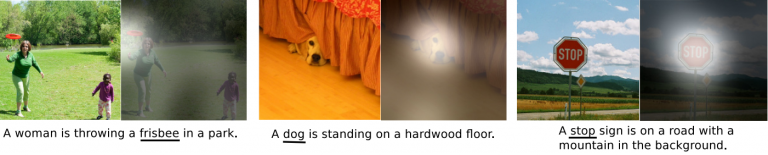
\includegraphics[scale=.5]{figures/gambar3}}
        \caption{Gambar to Text}
		\label{gambar}
\end{figure}

Untuk menerapkan mekanisme attention, kami mengambil input dari setiap langkah waktu encoder tetapi memberi bobot pada langkah waktu. Pembobotan tergantung pada pentingnya langkah waktu tersebut bagi dekoder untuk menghasilkan kata berikutnya secara optimal dalam urutan, seperti yang ditunjukkan pada gambar \ref{attention}

\begin{figure}[H]
        \centerline{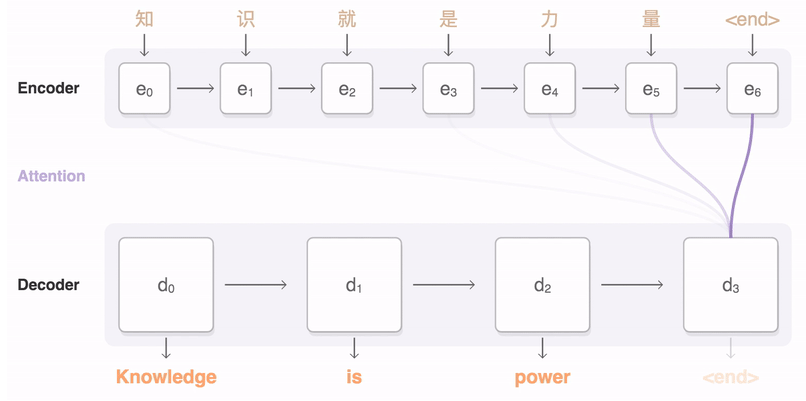
\includegraphics[scale=.5]{figures/gambar1}}
        \caption{Mekanisme Attention pada Gambar to Text}
		\label{attention}
\end{figure}


\subsection{Rumusan Masalah untuk Pemodelan Sequence to Sequence}
Kita tahu bahwa untuk memecahkan masalah pemodelan sequence, Jaringan Syaraf Tiruan adalah arsitektur terbaik yang dapat kita pilih. Mari kita ambil contoh Sistem Penjawab Pertanyaan untuk memahami seperti apa masalah pemodelan urutan. Misalkan terdapat serangkaian pernyataan sebagai berikut:

Jo pergi ke dapur. Fred pergi ke dapur. Joe mengambil susu itu.

Joe pergi ke kantor. Joe meninggalkan susu. Jo pergi ke kamar mandi.

Pertanyaannya dimana joe sebelum pergi ke kantor? Jawaban yang tepat adalah "dapur". Pandangan sekilas membuat ini tampak seperti masalah sederhana. Tetapi untuk memahami kompleksitasnya terdapat dua dimensi yang harus dipahami oleh sistem:

\begin{enumerate}
\item Pemahaman dalam bahasa Inggris dan urutan karakter/kata yang membentuk kalimat.
\item Urutan peristiwa yang berkisar pada orang-orang yang disebutkan dalam pernyataan.
\end{enumerate}
Ini dapat dianggap sebagai masalah pemodelan urutan, karena memahami urutan itu penting untuk membuat prediksi apa pun di sekitarnya. Ada banyak skenario masalah pemodelan urutan seperti itu, yang dirangkum dalam gambar di bawah ini. Contoh yang diberikan di atas adalah masalah banyak inputan dengan satu output (Jika Anda menganggap sebuah kata sebagai output tunggal).


\chapter{Speech Synthesis}
\section{Speech Synthesis}
Di berbagai media, Anda mungkin pernah menyaksikan Stephen Hawking berbicara di depan mahasiswanya. Fisikawan yang terkenal dengan teori black hole-nya ini sudah tidak mampu lagi mengeluarkan suara dari lisannya, namun berkat teknologi speech synthesizer, dia masih bisa bercakap-cakap. Mesin speech synthesizer Hawking memang cukup kompleks. Alat ini tidak hanya memproduksi suara, tetapi juga menangkap input dari gerakan mata sang doktor. Demikian pula, misalnya, dengan aplikasi voice command yang banyak tertanam di smartphone mutakhir yang memadukan speech recognizer dengan speech synthesizer.

Aplikasi speech synthesizer yang paling sederhana sebenarnya ada pada setiap PC ber-OS Windows. Bila anda menekan tuts Winkey + U di keyboard, Windows akan mengaktifkan Utility Manager, yang di dalamnya terdapat aplikasi Microsoft Narrator. Aplikasi ini akan membaca setiap jendela yang anda aktifkan, termasuk tombol-tombol di dalamnya. Atau, mungkin anda pernah menginstal aplikasi microsoft reader di PC. Aplikasi yang diperuntukkan bagi file >LTT ini pun dilengkapi dengan kemampuan menerjemahkan teks menjadi suara (text to speech) yang merupakan contoh teknologi speech synthesizer.

\begin{figure}[H]
        \centerline{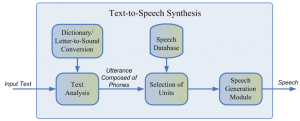
\includegraphics[scale=.75]{figures/speech}}
        \caption{Speech Synthesis}
		\label{speech}
\end{figure}

Speech synthesis adalah sebuah kemampuan bicara manusia yang dibuat oleh manusia (artificial). Sebuah sistem komputer digunakan untuk tujuan ini yang disebut sebagai speech synthesizer, dan dapat diimplementasikan ke dalam software atau hardware. Sebagai contoh sebuah sistem text-to-speech (TTS) yang dapat mengkonversikan teks dengan bahasa biasa menjadi suara.

Sebuah sistem komputer yang digunakan untuk tujuan ini disebut speech synthesizer, dan dapat diimplementasikan dalam perangkat lunak atau perangkat keras produk. Sebuah teks-to-speech (TTS) sistem mengkonversi teks bahasa normal menjadi berbicara; sistem lain membuat representasi linguistik simbolik seperti transkripsi fonetik ke dalam pidato, pidato disintesis dapat dibuat dengan menggabungkan potongan pidato direkam yang disimpan dalam database. Sistem berbeda dalam ukuran unit pidato disimpan, sebuah sistem yang menyimpan telepon atau diphones menyediakan berbagai keluaran terbesar, tapi mungkin kurang jelas.

Speech synthesis adalah transformasi dari teks ke arah suara (speech). Transformasi ini mengkonversi teks ke pemadu suara (speech synthesis) yang sebisa mungkin dibuat menyerupai suara nyata, disesuaikan dengan aturan – aturan pengucapan bahasa.TTS (text to speech) dimaksudkan untuk membaca teks elektronik dalam bentuk buku, dan juga untuk menyuarakan teks dengan menggunakan pemaduan suara. Sistem ini dapat digunakan sebagai sistem komunikasi, pada sistem informasi referral, dapat diterapkan untuk membantu orang-orang yang kehilangan kemampuan melihat dan membaca.

Synthesized speech dapat diciptakan dengan menggabungkan beberapa potongan-potongan dari pembicaraan/pidato yang sudah direkam dalam sebuah basis data. Kualitas dari sebuah speech synthesizer dilihat dari kemiripannya dengan suara manusia dan kemampuannya untuk bisa dipahami. Program TTS yang jelas dapat membantu orang dengan gangguan visual atau ketidakmampuan membaca, untuk mendengarkan pada pekerjaan yang tertulis dalam komputer. Banyak Sistem Operasi komputer yang telah dimasukkan speech synthesizer sejak tahun 1980-an.

Sebuah sistem text-to-speech (atau “mesin”) terdiri dari dua bagian: front-end dan back-end . Front-end memiliki dua tugas utama. Pertama, mengubah teks mentah berisi simbol seperti angka dan singkatan menjadi setara dengan kata-kata tertulis-out. Proses ini sering disebut normalisasi teks, pra-pengolahan, atau tokenization . Front-end kemudian memberikan transkripsi fonetik untuk setiap kata, dan membagi dan menandai teks ke unit prosodi , seperti frase , klausa , dan kalimat . Proses menetapkan transkripsi fonetik untuk kata-kata ini disebut teks-ke-fonem atau grafem konversi -untuk-fonem. Transkripsi fonetik dan informasi prosodi bersama-sama membentuk representasi linguistik simbolik yang output dengan front-end. Back-end-sering disebut sebagai synthesizer-maka mengubah representasi linguistik simbolik menjadi suara. Dalam sistem tertentu, bagian ini meliputi perhitungan dari target prosodi (kontur pitch, durasi fonem), yang kemudian dikenakan pada pidato output.

\subsection{Sejarah Speech Synthesis}
Upaya yang paling awal untuk menghasilkan lahirnya pemandu suara, pada abad XVIII. Terlepas dari kenyataan bahwa upaya pertama  adalah bentuk mesin mekanis, kita dapat mengatakan hari ini  bahwa synthesizer sudah berkualitas tinggi. Pada tahun 1779 di

St Petersburg, Rusia Profesor Kratzenshtein Kristen  fisiologis menjelaskan perbedaan antara lima vokal panjang  (/ A /, / e /, / i /, / o /, dan / u /) dan membuat alat untuk menghasilkan  mereka artifisial. Tahun 1791 di Wina, Wolfgang von Kempelen memperkenalkan nya “Akustik-Mekanik Mesin Speech”. Dalam  sekitar pertengahan 1800-an Charles Wheatstone dibangun terkenal  versi mesin berbicara von Kempelen’s.

Generasi dari sistem pemaduan suara ini dapat dibagi ke dalam 3 masa, yaitu:

\begin{enumerate}
\item Generasi pertama (1962-1977). Format sintesis dari fonem adalah teknologi dominan. Teknologi ini memanfaatkan aturan berdasarkan penguraian fonetik pada kalimat untuk kontur frekuensi forman. Beberapa sintesis masih miskin atau kurang dalam kejelasan dan kealamiannya.
\item Generasi kedua (1977-1992). Metode pemadu suara adalah diphone diwakilkan  dengan parameter LPC. Hal tersebut menunujukkan bahwa kejelasan yang baik pada pemadu suara dapat diperoleh dengan andal dari input teks dengan menggabungkan diphone yang sesuai dengan unit. Kejelasan meningkat selama sintesis forman, tetapi kealamian dari pemadu suara masih tetap rendah.
\item Generasi ketiga (1992-sekarang). Generasi ini ditandai dengan metode ‘ sintesis pemilihan unit’ yang diperkenalkan dan disempurnakan oelh Sagisaka di Labs ATR Kyoto. Hasil dari pemandu suara pada periode ini sangat mendekati human-generated speech pada bagian kejelasan dan kealamian.
\end{enumerate}

Teknologi pemadu suara modern melibatkan metode dan algoritma yang canggih dan rumit. alat pemadu suara  dari keluarga “Infovox” mungkin mejadi salah satu multi bahasa TTS yang paling dikenal saat ini. Versi komersial pertamanya, Infovox-SA 101, dikembangkan pada tahun 1982 di Institute Teknologi Royal, Swedia dan didasarkan pada sintesis forman.

AT \& T Bell Laboratories (Lucent Technologies) juga memiliki tradisi yang sangat panjang tentang pemandu suara (speech synthesis). TTS lengkap yang pertama didemostrasikan di Boston pada tahun 1972 dan diliris pada tahun 1973. Hal ini didasarkan pada model artikulatoris yang sikembangkan oleh Ceceil Coker (Klatt 1987). Pengembangan proses dari sistem penggabungan sintesis ini dimulai oleh Joseph Olive pada pertengahan tahun 1970-an (Bell Labs 1997). Sistem ini sekarang sudah tersedia untuk bahasa Inggris, Perancis, Spanyol, Italia, Jerman, Rusia, Rumania, Cina, dan Jepang (Mcbius et al 1996).

\begin{figure}[H]
        \centerline{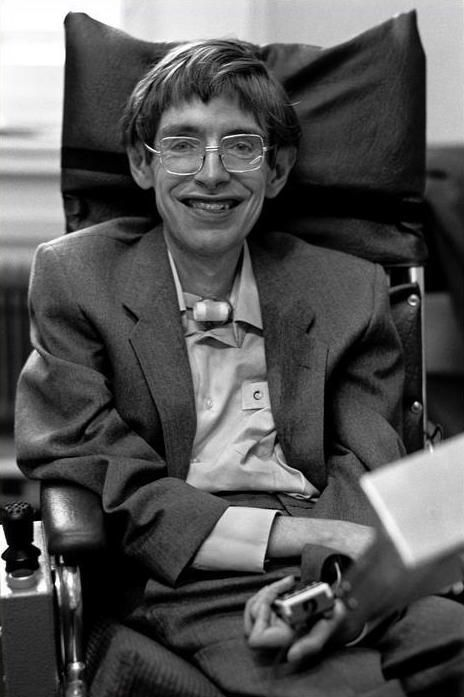
\includegraphics[scale=.45]{figures/stephan}}
        \caption{Stephen Hawking adalah salah satu orang paling terkenal yang menggunakan sintesis ucapan untuk berkomunikasi}
		\label{stephan}
\end{figure}

\subsection{Perangkat Speech Synthesis}
Pidato sistem sintesis berbasis komputer pertama diciptakan pada akhir 1950-an. Pertama umum Inggris sistem text-to-speech dikembangkan oleh Noriko Umeda et al. Pada tahun 1968 di Laboratorium Elektroteknik, Jepang. Pada tahun 1961, fisikawan John Larry Kelly, Jr dan Louis rekan Gerstman menggunakan IBM 704 komputer untuk mensintesis pidato, acara yang paling menonjol dalam sejarah Bell Labs . Kelly perekam suara synthesizer ( vocoder ) ulang lagu ” Daisy Bell “, dengan iringan musik dari Max Mathews .Kebetulan, Arthur C. Clarke mengunjungi teman dan kolega John Pierce di fasilitas Bell Labs Murray Hill. Clarke begitu terkesan oleh demonstrasi bahwa ia digunakan dalam adegan klimaks dari skenario-Nya untuk novel nya 2001: A Space Odyssey, di mana HAL 9000 komputer menyanyikan lagu yang sama seperti yang sedang ditidurkan oleh astronot Dave Bowman. Meskipun keberhasilan pidato sintesis murni elektronik, penelitian masih terus dilakukan ke synthesizer pidato mekanis.

Handheld elektronik menampilkan sintesis pidato mulai muncul pada 1970-an. Salah satu yang pertama adalah Telesensory Systems Inc(TSI) Pidato + kalkulator portabel untuk orang buta pada tahun 1976. Perangkat lain yang diproduksi terutama untuk tujuan pendidikan, seperti Bicara \& Eja , yang diproduksi oleh Texas Instruments pada tahun 1978. Fidelity merilis versi berbicara komputer catur elektronik pada tahun 1979. Yang pertama video game yang memiliki fitur sintesis pidato adalah 1.980 shoot ’em up arcade game , Stratovox , dari Sun Electronics. Contoh lain awal adalah versi arcade dari Berzerk , dirilis pada tahun yang sama.Pertama multi-player permainan elektronik menggunakan sintesis suara adalah Milton dari Milton Bradley Company , yang memproduksi perangkat di tahun 1980.

\subsection{Teknologi Speech Synthesis}
Yang paling penting dalam kualitas sistem speech synthesis adalah kealamian dan kejelasannya. Kealamaian menjelaskan bagaimana dekatnya suara output dengan suara manusia, sementara kejelasan adalah dengan kemudahan di mana output tersebut dapat dipahami. Speech synthesizer yang ideal adalah yang alami dan jelas. Sistem speech synthesis biasanya mencoba untuk memaksimalkan kedua karakteristik.

Kualitas terpenting dari sebuah aplikasi speech synthesizer adalah seberapa alami dan inteligibel output yang dihasilkannya. Alami, artinya seberapa dekat suara yang dihasilkan aplikasi speech synthesizer dengan suara manusia. Sedangkan inteligibel adalah seberapa mudah output tersebut dipahami oleh manusia. Semua aplikasi speech synthesizer berusaha untuk menghasilkan output yang alami dan inteligibel sekaligus.

Sampai saat ini, ada banyak teknologi untuk meng-generate gelombang suara sintetis ini. Dua teknologi yang paling banyak digunakan adalah concatenative synthesis dan formant synthesis. Keduanya memiliki keunggulan dan kekurangan sendiri-sendiri.

Teknologi pertama, concatenative synthesis, berbasis pada rangkaian (atau merangkai bersama) segmen-segmen dari suara yang direkam. Umumnya, teknologi ini menghasilkan suara sintesis yang terdengar paling alami.Namun, perbedaan antara suara alami yang direkam dengan segmentasi gelombang bunyi kadang menghasilkan suara yang menggangu. Mirip seperti suara pemberitahuan nomor antrean di bank atau suara call center operator ponsel yang menyebutkan sisa pulsa dan masa berlaku kartu ponsel anda.

Teknologi kedua, formant synthesis, tidak menggunakan sampel suara manusia melainkan membuat suara sintesi menggunakan model akustik. Parameter-parameter seperti frekuensi dasar, alunan suara, dan tingkat kebisingan bervariasi dari waktu ke waktu untuk menciptakan gelombang suara buatan.

Kebanyakan aplikasi berbasis teknologi ini menghasilkan suara buatan (tidak alami) seperti suara robot. Melihat keterbatasan kedua teknologi ini dalam menghasilkan suara buatan, seperti kita harus sabar menunggu pengembangannya lebih lanjut dalam beberapa tahun atau dekade ke depan.

Kualitas yang paling penting dari sebuah sistem sintesis pidato kewajaran dan dimengerti. kealamian menjelaskan seberapa dekat output terdengar seperti suara manusia, sementara kejelasan adalah kemudahan yang output dipahami. Speech synthesizer yang ideal adalah baik alam dan dimengerti. Sistem sintesis pidato biasanya mencoba untuk memaksimalkan kedua karakteristik.

Dua teknologi utama dalam pembuatan gelombang suara synthetic speech adalah Concatenative Synthesis dan Formant Synthesis. Setiap teknologi mempunyai kekuatan dan kelemahannya, dan penggunaan yang ditujukan dari sistem synthesis akan menentukkan pendekatan mana yang digunakan.

\begin{enumerate}
\item Concatenative Synthesis
Concantenative synthesis didasarkan dengan penggabungan dari segmen-segmen dari pembicaraan yang sudah direkam. Secara umum, concatenative synthesis memproduksi synthesized speech dengan suara yang paling alami. Tetapi, perbedaan antara variasi alami dalam pembicaraaan dan sifat dari teknik otomasi untuk pensegmentasian gelombang suara terkadang menghasilkan kesalahan suara dalam output. Namun, perbedaan antara variasi alami dalam pidato dan sifat teknik otomatis untuk membagi bentuk gelombang kadang-kadang menyebabkan gangguan terdengar pada output. Ada tiga sub-jenis utama dari sintesis concatenative.
\begin{enumerate}
\item Sintesis Pemilihan unit
Sintesis Pemilihan unit menggunakan besar database pidato direkam. Selama pembuatan database, setiap ucapan tercatat tersegmentasi ke dalam beberapa atau semua hal berikut: individu telepon , diphones , setengah-telepon, suku kata , morfem , kata , frase , dan kalimat . Biasanya, pembagian ke dalam segmen dilakukan dengan menggunakan dimodifikasi khusus recognizer pidato disetel ke “keselarasan dipaksa” mode dengan beberapa koreksi manual setelah itu, dengan menggunakan representasi visual seperti yang gelombang dan spektogram .  Sebuah indeks unit dalam database pidato kemudian dibuat berdasarkan segmentasi dan parameter akustik seperti frekuensi dasar (lapangan ), durasi, posisi dalam suku kata, dan telepon tetangga. Pada waktu berjalan , target ucapan yang diinginkan dibuat dengan menentukan rantai terbaik unit calon dari database (pemilihan unit). Proses ini biasanya dicapai dengan menggunakan khusus tertimbang pohon keputusan.

Pemilihan unit menyediakan kealamian terbesar, karena hanya berlaku sedikit pemrosesan sinyal digital (DSP) untuk pidato direkam. DSP sering membuat pidato yang direkam terdengar kurang alami, meskipun beberapa sistem menggunakan sejumlah kecil pengolahan sinyal pada titik Rangkaian untuk menghaluskan bentuk gelombang. Output dari yang terbaik unit-seleksi sistem sering dibedakan dari suara manusia nyata, terutama dalam konteks dimana sistem TTS telah disetel. Namun, kealamian maksimum biasanya membutuhkan unit-pilihan database pidato menjadi sangat besar, dalam beberapa sistem mulai ke gigabyte data dicatat, mewakili puluhan jam berbicara.  Juga, pilihan algoritma Unit telah dikenal untuk memilih segmen dari Tempat yang menghasilkan kurang dari sintesis ideal (misalnya kata-kata kecil menjadi tidak jelas) bahkan ketika pilihan yang lebih baik ada dalam database. Baru-baru ini, peneliti telah mengusulkan berbagai metode otomatis untuk mendeteksi segmen alami di unit-pilihan sistem sintesis pidato.
\item Sintesis diphone
Sintesis diphone menggunakan database pidato minimal berisi semua diphones (suara-to-suara transisi) yang terjadi dalam suatu bahasa. Jumlah diphones tergantung pada fonotaktik bahasa: misalnya, Spanyol memiliki sekitar 800 diphones, dan Jerman sekitar 2500. Dalam sintesis diphone, hanya satu contoh dari setiap diphone terkandung dalam database pidato. Pada saat runtime, target prosodi kalimat ditumpangkan pada unit-unit minimal dengan cara pemrosesan sinyal digital teknik seperti linear predictive coding ,PSOLA atau MBROLA. Diphone sintesis menderita gangguan sonik sintesis concatenative dan robot-terdengar sifat sintesis forman, dan memiliki beberapa keuntungan baik pendekatan lain dari ukuran kecil. Dengan demikian, penggunaannya dalam aplikasi komersial menurun, meskipun terus digunakan dalam penelitian karena ada beberapa implementasi perangkat lunak tersedia secara bebas.
\item Domain-spesifik sintesis
Domain-spesifik sintesis concatenates direkam sebelumnya kata dan frase untuk menciptakan ucapan-ucapan yang lengkap. Hal ini digunakan dalam aplikasi di mana berbagai teks output sistem akan terbatas pada domain tertentu, seperti jadwal angkutan pengumuman atau laporan cuaca.  Teknologi ini sangat sederhana untuk menerapkan, dan telah digunakan secara komersial untuk waktu yang lama , dalam perangkat seperti berbicara jam dan kalkulator. Tingkat kealamian sistem ini bisa sangat tinggi karena berbagai jenis kalimat terbatas, dan mereka cocok dengan prosodi dan intonasi dari rekaman asli.

Karena sistem ini dibatasi oleh kata-kata dan frasa dalam database mereka, mereka tidak tujuan umum dan hanya dapat mensintesis kombinasi kata dan frase yang mereka telah terprogram. Campuran kata-kata dalam bahasa alami diucapkan namun masih dapat menyebabkan masalah kecuali banyak variasi diperhitungkan. Misalnya, dalam non-rhotic dialek dari bahasa Inggris “r” dalam kata-kata seperti “jelas” biasanya hanya diucapkan ketika kata berikut memiliki vokal sebagai huruf pertama (misalnya”membersihkan” direalisasikan sebagai  ). Demikian juga di Perancis , banyak konsonan akhir menjadi tidak lagi diam jika diikuti oleh sebuah kata yang dimulai dengan vokal, efek yang disebut penghubung . Ini pergantian tidak bisa direproduksi oleh sistem kata-Rangkaian sederhana, yang akan membutuhkan kompleksitas tambahan untuk konteks-sensitif .
\end{enumerate}
\item Formant Synthesis
Formant synthesis tidak menggunakan pembicaraan manusia sebagai sample pada runtime. Daripada itu, synthesized speech yang dihasilkan dibuat dengan additive synthesis dan sebuah model akustik (physical modelling synthesis).

Parameter seperti frekuensi dasar, penyuaraan, dan tingkat kebisingan di variasikan dari waktu ke waktu untuk menciptakan gelombang buatan (artificial) dari sebuah pembicaraan. Banyak sistem yang berdasarkan formant synthesis menciptakan pembicaraan yang seperti robot yang tidak mungkin dapat dikenal sebagai suara manusia. Tetapi, kealamian maksimum bukan selalu tujuan dari sebuah sistem speech synthesis, dan sistem formant synthesis mempunyai keuntungan dari sistem concatenative. Pembicaraan yang di-formant synthesis-kan dapat menjadi sangat jelas, bahkan dalam kecepatan yang tinggi, sehingga menghindari kesalahan suara yang sering dialami sistem concatenative.

Formant synthesis biasanya program yang lebih kecil dari concatenative sistem karena ia tidak menggunakan basis data dari sampel-sampel pembicaraan. Oleh karena itu formant synthesis dapat ditanamkan dalam sistem yang mempunyai memory dan microprosesor yang terbatas. Karena sistem yang berdasarkan formant mempunyai kendali penuh dari sluruh aspek dari hasil pembicaraan, variasi yang luas dari prosodi dan intonasi dapat dihasilkan, menyampaikan tidak hanya pertanyaan dan pernyataan tetapi juga emosi dan nada suara.

Formant sintesis tidak menggunakan sampel suara manusia pada saat runtime. Sebaliknya, keluaran suara yang disintesis dibuat menggunakan aditif sintesis dan model akustik (sintesis pemodelan fisik ). Parameter seperti frekuensi dasar , menyuarakan , dan kebisingan tingkat yang bervariasi dari waktu ke waktu untuk membuat gelombang pidato buatan. Metode ini kadang-kadang disebut aturan berbasis sintesis; Namun, banyak sistem concatenative juga memiliki aturan berbasis komponen. Banyak sistem yang didasarkan pada teknologi sintesis forman menghasilkan buatan, robot yang terdengar pidato yang tidak akan pernah salah untuk pidato manusia. Namun, kealamian maksimum tidak selalu tujuan sistem sintesis pidato, dan sistem sintesis forman memiliki keunggulan dibandingkan sistem concatenative. Pidato forman-disintesis dapat diandalkan dimengerti, bahkan pada kecepatan yang sangat tinggi, menghindari Glitches akustik yang biasanya wabah sistem concatenative. Kecepatan tinggi disintesis pidato digunakan oleh tunanetra untuk navigasi cepat komputer menggunakan pembaca layar . Synthesizer forman adalah program biasanya lebih kecil dibandingkan dengan sistem concatenative karena mereka tidak memiliki database contoh pidato. Karena itu mereka dapat digunakan dalam embedded system , di mana memori dan mikroprosesor daya terutama terbatas. Karena sistem berbasis forman memiliki kontrol penuh dari semua aspek pidato output, berbagai prosodies dan intonasi dapat menjadi output, tidak hanya menyampaikan pertanyaan dan pernyataan, tetapi berbagai emosi dan nada suara.

Contoh non-real-time tapi sangat akurat kontrol intonasi dalam sintesis forman meliputi pekerjaan yang dilakukan pada akhir tahun 1970 untuk Texas Instruments mainan Bicara \& Eja , dan pada awal tahun 1980 Sega arcade mesin dan dalam banyak Atari, Inc. game arcade menggunakan TMS5220 LPC Chips . Menciptakan intonasi yang tepat untuk proyek ini adalah telaten, dan hasilnya masih harus dicocokkan dengan real-time text-to-speech interface.
\item Sintesis artikulatoris
Sintesis artikulatoris mengacu pada teknik komputasi untuk sintesis pidato berdasarkan model manusia saluran vokal dan artikulasi proses yang terjadi di sana. Synthesizer artikulatoris pertama teratur digunakan untuk percobaan laboratorium dikembangkan di Haskins Laboratories di pertengahan 1970-an oleh Philip Rubin, Tom Baer, dan Paul Mermelstein. Synthesizer ini, yang dikenal sebagai ASY, didasarkan pada model saluran vokal dikembangkan di Bell Laboratories pada tahun 1960 dan 1970-an oleh Paul Mermelstein, Cecil Coker, dan rekan.

Sampai saat ini, model sintesis artikulatoris belum dimasukkan ke dalam sistem sintesis pidato komersial. Sebuah pengecualian adalah NeXT sistem berbasis awalnya dikembangkan dan dipasarkan oleh Trillium Suara Research, sebuah perusahaan spin-off dari University of Calgary , di mana banyak riset asli dilakukan. Setelah runtuhnya berbagai inkarnasi NeXT (dimulai oleh Steve Jobs pada akhir tahun 1980 dan bergabung dengan Apple Computer pada tahun 1997), perangkat lunak TRILLIUM diterbitkan di bawah GNU General Public License , dengan bekerja terus sebagai gnuspeech . Sistem, pertama kali dipasarkan pada tahun 1994, memberikan penuh text-to-speech konversi berbasis artikulatoris menggunakan Waveguide atau transmisi-line analog dari saluran mulut dan hidung manusia dikendalikan oleh Carré ini “model daerah khas”.
\item Sintesis berbasis HMM
Sintesis berbasis HMM  adalah metode sintesis berdasarkan model Markov tersembunyi , juga disebut statistik Parametrik Sintesis. Dalam sistem ini, spektrum frekuensi ( vokal ),frekuensi dasar (sumber vokal), dan durasi ( prosodi ) berbicara dimodelkan secara bersamaan oleh HMMs. Pidato bentuk gelombang yang dihasilkan dari HMMs sendiri berdasarkan maksimum kriteria.
\item Sintesis Sinewave
Sintesis sinewave adalah teknik untuk sintesis pidato dengan mengganti forman (band utama energi) dengan peluit nada murni.

Ada beberapa masalah yang terdapat pada pemaduan suara, yaitu:
\begin{enumerate}
\item User sangat sensitif terhadap variasi dan informasi suara. Oleh sebab itu, mereka tidak dapat memberikan toleransi atas ketidaksempurnaan pemadu suara.
\item Output dalam bentuk suara tidak dapat diulang atau dicari dengan mudah.
\item Meningkatkan keberisikan pada lingkungan kantor atau jika menggunakan handphone, maka akan meningkatkan biaya pengeluaran.
\end{enumerate}
\end{enumerate}


\chapter{Voice Cloning}
\section{Voice Cloning}
Kloning suara sering diombang-ambingkan dengan istilah lain, seperti suara deepfake, sintesis ucapan, dan suara sintetis, yang memiliki arti yang sedikit berbeda. Kloning suara adalah proses di mana seseorang menggunakan komputer untuk menghasilkan ucapan individu nyata, menciptakan tiruan dari suara mereka yang spesifik dan unik menggunakan kecerdasan buatan (AI)\cite{8999436}. Sistem text-to-speech (TTS), yang dapat mengambil bahasa tertulis dan mengubahnya menjadi komunikasi lisan, tidak sama dengan kloning suara. Sistem TTS jauh lebih terbatas dari output yang mereka hasilkan dibandingkan dengan teknologi kloning suara, yang sebenarnya lebih merupakan proses kustom. Dengan sistem TTS, data pelatihan, komponen kunci untuk setiap media yang dibuat secara sintetis, menginformasikan produksi keluaran suara. Dengan kata lain, suara yang Anda dengar adalah suara yang diberikan dalam kumpulan data. Sekarang, dengan diperkenalkannya teknologi AI kloning suara, itu berubah. Metode telah diterapkan untuk memberikan analisis yang lebih dalam dan ekstraksi karakteristik suara target. Atribut-atribut ini kemudian dapat diterapkan pada bentuk gelombang ucapan yang berbeda, memungkinkan seseorang untuk mengubah keluaran suara dari satu suara ke suara lainnya\cite{9239750}.

\begin{figure}[H]
        \centerline{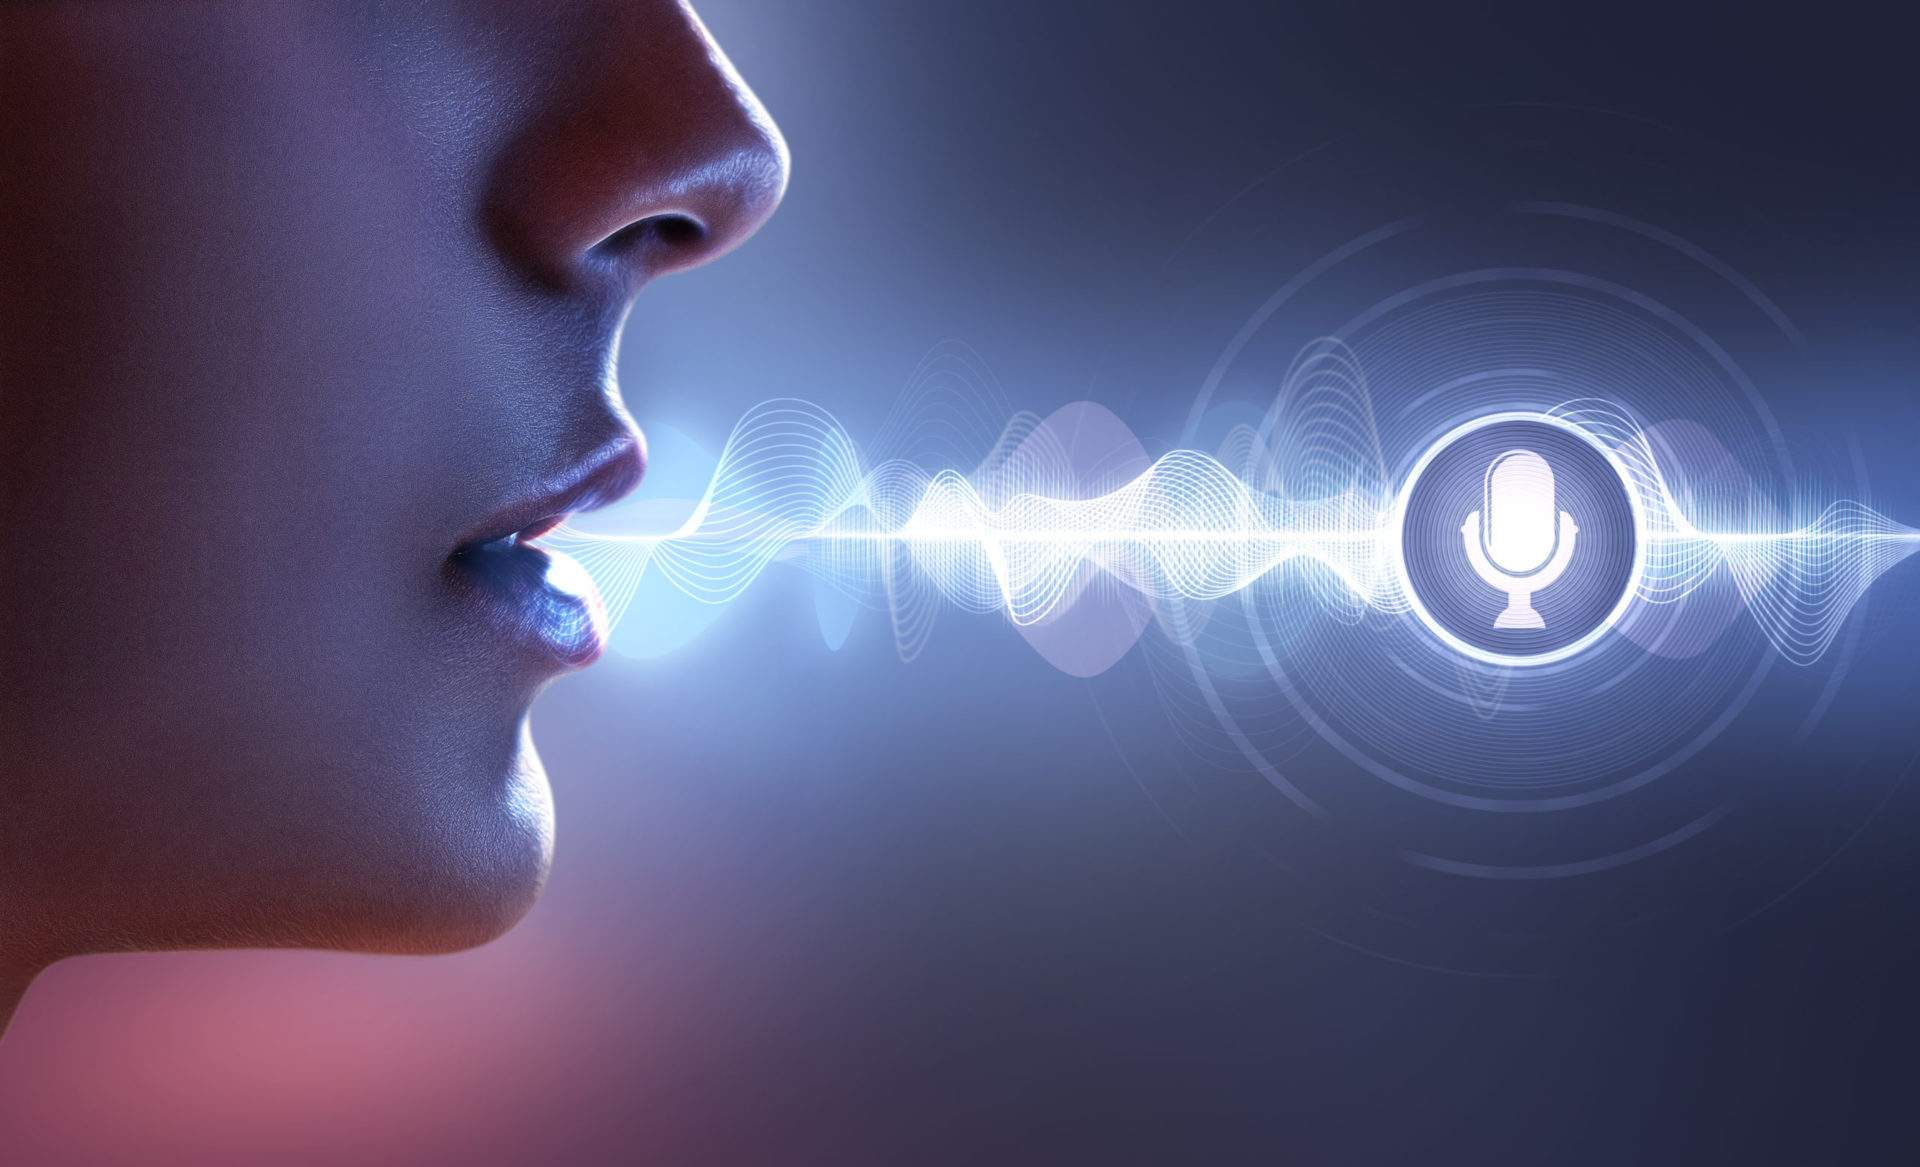
\includegraphics[scale=.15]{figures/voicecloning}}
        \caption{Voice Cloning}
		\label{voicecloning}
\end{figure}

Berkat kemajuan dalam kecerdasan buatan (AI), khususnya pembelajaran mendalam, bagian dari pembelajaran mesin di bawah payung AI, kami telah mampu menghasilkan replika suara yang akurat. Tapi ini hanya dimungkinkan oleh dua hal:

\begin{enumerate}
\item Perangkat keras yang kuat dengan kemampuan komputasi awan untuk memproses dan merender secara tepat waktu dan efisien
\item Data pelatihan ekstensif dari suara yang ditargetkan dari mana model dapat memanfaatkan untuk membuat klon suara yang akurat
\end{enumerate}

Dengan AI yang tepat dan keahlian dan alat pengembangan, itu benar-benar tergantung pada yang terakhir. Anda memerlukan sejumlah besar ucapan yang direkam untuk memiliki data yang cukup untuk melatih model suara. Informasi seputar suara disimpan dalam embedding , ruang berdimensi cukup rendah di mana Anda dapat menerjemahkan variabel diskrit menjadi vektor berdimensi tinggi. Dengan kata lain, lebih mudah untuk bekerja dengan input besar dengan model pembelajaran mesin. Agar tidak terlalu teknis, kami akan berhenti di situ, tetapi jangan ragu untuk menyelam lebih dalam ke subjek jika itu menarik minat Anda.

\subsection{Manfaat Voice Cloning}
Mari kita mulai dengan yang baik. Ada banyak kasus penggunaan potensial untuk kloning suara yang sering kali dibayangi oleh penggunaan negatif, yang akan kita bahas sebentar lagi. Beberapa aplikasi positif dari teknologi meliputi:

\begin{enumerate}
\item Meningkatkan peluang iklan dan sponsor untuk pengisi suara, selebritas, dan influencer
\item Bantu perusahaan bekerja dengan talenta selama waktu tersibuk mereka dalam setahun, seperti musim sepak bola untuk pemain atau pelatih
\item Menghidupkan kembali suara-suara dari masa lalu untuk digunakan dalam hiburan guna membantu menceritakan kisah dalam dokumenter, film, dan acara TV
\item Diversifikasi konten siaran untuk konten berulang seperti laporan cuaca atau pembaruan olahraga
\item Lokalkan konten sehingga dapat didengar dalam suara pembawa acara atau narator dalam bahasa lain
\end{enumerate}

Ini hanyalah beberapa kegunaan positif dari kloning suara, dan seiring dengan berkembangnya teknologi, lebih banyak lagi yang akan muncul. Tapi tentu saja, semuanya bergantung pada etika penggunaan suara seseorang. Itulah mengapa perlunya gerakan menuju standarisasi proses persetujuan sangat penting untuk melindungi suara semua orang dan memastikan mereka memiliki kendali penuh atas cara penggunaannya.

\subsection{Aplikasi Voice Cloning Terbaik}

\begin{figure}[H]
        \centerline{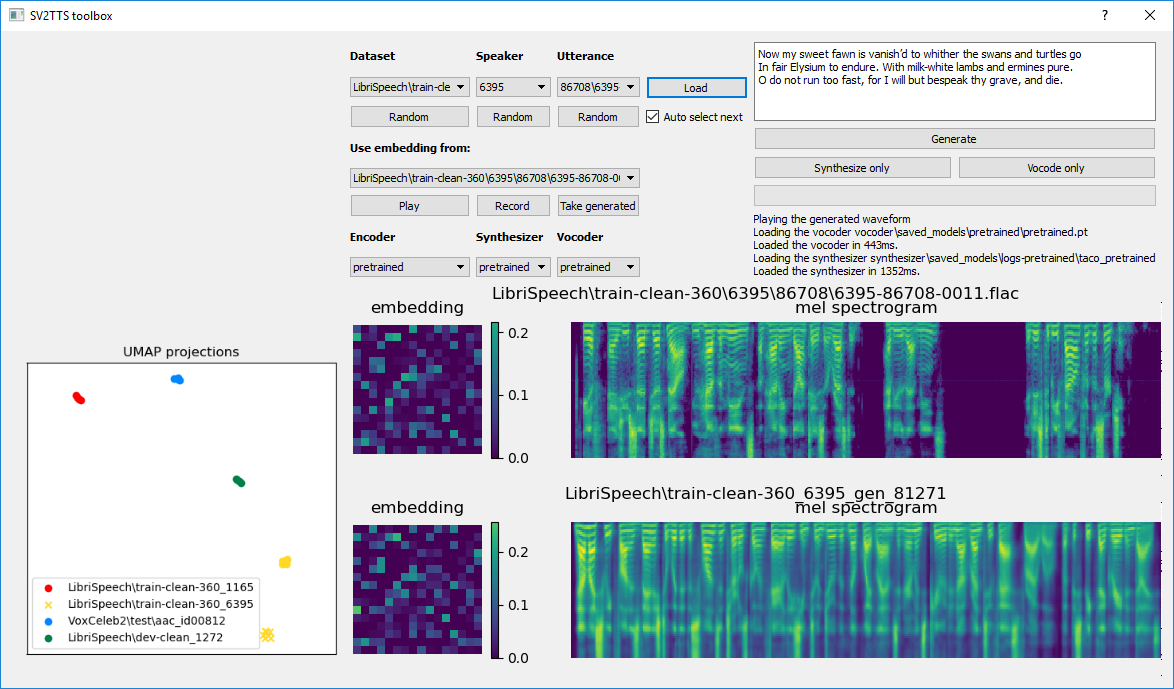
\includegraphics[scale=.35]{figures/voice-clone}}
        \caption{Contoh Aplikasi Voice Cloning (SV2TTS Toolbox)}
		\label{appvoice}
\end{figure}

Untuk mempersempit pencarian Anda untuk menemukan aplikasi kloning suara terbaik, Anda harus terlebih dahulu menentukan apa yang Anda cari. Apakah Anda memerlukan sesuatu yang lebih untuk output text-to-speech? Atau apakah Anda membutuhkan sesuatu yang lebih khusus?

Setelah Anda mengetahui mengapa Anda memerlukan aplikasi kloning suara, Anda harus mengasah tiga kriteria utama:
\begin{enumerate}
\item Kualitas keluaran: Anda pasti ingin memastikan bahwa keluaran terdengar otentik dan memenuhi kebutuhan yang ditentukan. Biasanya, mereka akan memiliki sampel tentang apa yang dapat dilakukan produk tersebut. Jika tidak, Anda harus mempertimbangkan untuk meminta demo, jika tersedia, untuk menentukan seberapa manusiawi produk mereka.

\item Antarmuka intuitif: seberapa mudah menggunakan aplikasi? Apakah sulit untuk menemukan sesuatu saat Anda berada di aplikasi atau dapatkah Anda menavigasi dan menggunakannya untuk memenuhi kebutuhan Anda? Sekali lagi, ini dapat ditentukan oleh video produk, konten pemasaran, dan demo.

\item Perlindungan suara: Anda pasti ingin memastikan bahwa perusahaan mengikuti penggunaan suara yang etis. Jika itu adalah layanan kustom yang memerlukan data pelatihan, maka penting untuk menanyakan tentang perlindungan data dan bagaimana suara, saat dibuat, tidak akan digunakan secara tidak semestinya.
\end{enumerate}

Implikasi etis seputar kloning suara adalah hubungan dari Veritone MARVEL.ai, aplikasi suara sebagai layanan kami . Dibangun dalam kerangka aplikasi adalah tuas untuk memberi pengguna kendali atas suara mereka, memungkinkan perlindungan yang tepat sehingga mereka memutuskan siapa yang dapat menggunakan suara mereka. Ini membantu kami memberikan solusi voice-as-a-service khusus kami untuk memungkinkan pengalaman sarung tangan putih lengkap untuk talenta yang bekerja dengan kami.

\subsection{Pembuatan Voice Cloning}
Perangkat lunak kloning suara AI online dimulai dengan menggunakan komputer untuk mensintesis suara. Text-to-Speech (TTS) adalah teknologi berusia puluhan tahun yang mengubah teks menjadi ucapan sintetis, memungkinkan suara digunakan untuk interaksi komputer-manusia.

Di masa lalu ada dua pendekatan untuk TTS. Yang pertama, TTS Concatenative\cite{Hunt1996UnitSI}, menggunakan rekaman audio untuk membuat perpustakaan kata dan satuan suara (fonem) yang dapat dirangkai menjadi kalimat. Meskipun keluarannya berkualitas tinggi dan dapat dipahami, ia tidak memiliki emosi dan infleksi yang ditemukan dalam ucapan manusia yang alami. Saat menggunakan TTS Concatenative, setiap gaya bicara atau bahasa baru memerlukan database audio baru. Dan tentu saja upaya untuk mengkloning suara individu menggunakan metode ini membutuhkan investasi yang sangat besar, biasanya hanya dilakukan untuk mendukung suara bermerek.

Pendekatan kedua adalah Parametrik TTS\cite{ZEN20091039}, metode yang menggunakan model statistik ucapan untuk menyederhanakan pembuatan suara, mengurangi biaya dan upaya dibandingkan dengan Penggabungan. Namun, upaya untuk menciptakan satu suara apa pun secara historis mahal, dan hasilnya jelas bukan manusia.

Saat ini, Kecerdasan Buatan (AI) dan kemajuan dalam Pembelajaran Mendalam meningkatkan kualitas ucapan sintetis. Pengajuan TTS sekarang sudah lumrah. Setiap orang yang telah berinteraksi dengan sistem Respon Suara Interaktif berbasis telepon, Siri Apple, Amazon Alexa, sistem navigasi mobil, atau banyak antarmuka suara lainnya, telah mengalami ucapan sintetis.

Jika Anda terbiasa dengan konsep video deepfake, perangkat lunak kloning suara AI online adalah setara dengan ucapan. Hanya dengan beberapa menit rekaman ucapan, pengembang dapat membangun kumpulan data audio dan menggunakannya untuk melatih model suara AI yang dapat membaca teks apa pun dalam suara target.

Pembuatan voice cloning secara signifikan menjadi lebih mudah berkat berbagai alat bertenaga jaringan saraf seperti Tacotron dan Wavenet atau Lyrebird Google, yang memungkinkan hampir semua suara direplikasi dan digunakan untuk "membaca" input teks. Kualitas output terus meningkat, seperti yang ditunjukkan oleh tiruan suara podcaster Joe Rogan ini. Insinyur pembelajaran mendalam di Dessa yang membuat klon juga menyiapkan kuis. Ambil untuk melihat apakah Anda dapat melihat Rogan palsu.

Model TTS berbasis jaringan saraf meniru cara otak beroperasi dan sangat efisien dalam mempelajari pola dalam data. Meskipun ada pendekatan berbeda untuk penggunaan pembelajaran mendalam dalam suara sintetis, sebagian besar menghasilkan pengucapan kata yang lebih baik, serta menangkap kehalusan seperti kecepatan dan intonasi untuk menciptakan ucapan yang lebih mirip manusia. 

Penting untuk dicatat bahwa alat yang disebutkan di atas dan alat lain seperti ini tidak dibuat untuk tujuan penipuan atau penipuan. Tetapi kenyataannya adalah bahwa bisnis dan konsumen perlu mewaspadai ancaman baru yang terkait dengan perangkat lunak kloning suara AI online. Kami menjelajahi beberapa kegunaan — baik dan buruk — di bawah ini. 

\subsection{Dampak Negatif Voice Cloning}
\begin{enumerate}
\item Voice adalah pengenal pribadi unik yang mudah diakses oleh penipu. Hal ini tentu berlaku bagi publik figur termasuk selebriti, politisi dan pemimpin bisnis, tetapi kenyataannya adalah siapa saja bisa menjadi sasaran. Video online, pidato, panggilan konferensi, percakapan telepon, dan posting media sosial semuanya dapat digunakan untuk mengumpulkan data yang diperlukan untuk melatih sistem untuk mengkloning suara.

\item Spoofing biometrik suara — Suara adalah pengidentifikasi unik dan ukuran yang andal untuk keamanan biometrik. Namun, penjahat dapat menggunakan serangan presentasi termasuk suara yang direkam, suara yang diubah komputer dan suara sintetis, atau kloning suara, untuk mengelabui sistem biometrik suara agar mengira mereka mendengar pengguna yang sebenarnya dan berwenang dan memberikan akses ke informasi dan akun sensitif.
\begin{figure}[H]
        \centerline{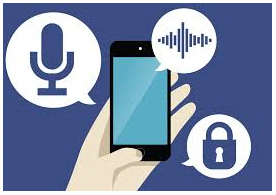
\includegraphics[scale=1]{figures/spoof}}
        \caption{Spoofing Voice Biometrics}
		\label{spoof}
\end{figure}

\item Penipuan phishing – Perangkat lunak kloning suara AI online juga memungkinkan jenis baru penipuan phishing yang mengeksploitasi fakta bahwa korban percaya bahwa mereka sedang berbicara dengan seseorang yang mereka percayai. Tahun lalu, seorang CEO yang berbasis di Inggris ditipu untuk mentransfer lebih dari \$240.000 berdasarkan panggilan telepon yang dia yakini berasal dari bosnya, CEO perusahaan induk organisasi Jerman.
\begin{figure}[H]
        \centerline{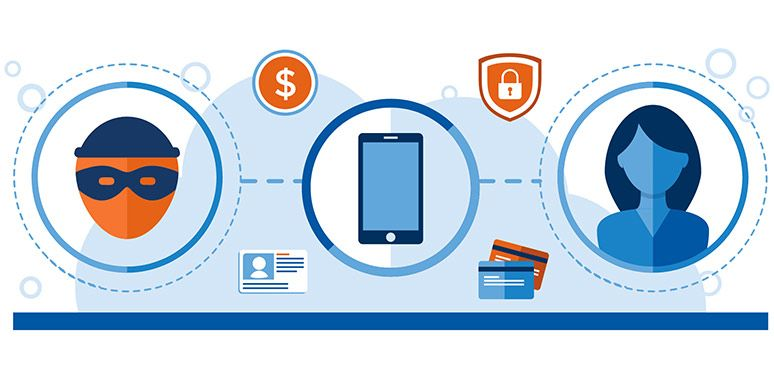
\includegraphics[scale=.4]{figures/voice-phising}}
        \caption{Voice Phising, Sumber: \url{https://id.pinterest.com/pin/195765915039905230/}}
		\label{phising}
\end{figure}

\item Penipuan seperti ini adalah evolusi penipuan email di mana email eksekutif dipalsukan dalam upaya agar penerima membocorkan nomor rekening bank, informasi kartu kredit, kata sandi, dan data sensitif lainnya. Sekarang scammers, dipersenjatai dengan klon suara, menggunakan panggilan telepon dan pesan suara. Dan serangan itu tidak hanya mengancam bisnis. Dalam generasi baru penjahat "mother's deception" menyamar sebagai anggota keluarga yang membutuhkan dana darurat.

\item Misinformasi – Berita palsu dan bentuk misinformasi serupa merupakan ancaman serius. Banyak dari kita yang akrab dengan bagaimana video yang dimanipulasi berdampak pada lanskap politik. Misalnya, video populer menunjukkan Barack Obama memanggil Trump – yah, anggap saja itu tidak terlalu bagus. Itu juga tidak nyata. Teknologi perangkat lunak text-to-speech berbasis AI akan semakin mendorong upaya ini untuk mempengaruhi opini publik, menghidupkan sumbangan kampanye palsu, mencemarkan nama baik tokoh masyarakat, dan banyak lagi. Di bidang bisnis, pertimbangkan bagaimana pernyataan eksekutif atau figur publik yang dimanipulasi dapat memengaruhi pasar saham.

\item Bukti – Suara sintetis dan deepfake lainnya dapat digunakan untuk membuat bukti palsu yang berdampak pada kasus kriminal. Meskipun ada pemeriksaan untuk memvalidasi bukti audio dan video yang disajikan di pengadilan, mencegah taktik ini memengaruhi kesaksian berdasarkan apa yang orang yakini mereka lihat atau dengar mungkin merupakan tantangan.

\item Pemerasan dan intimidasi – Video dan audio yang dimanipulasi dari orang-orang yang melakukan atau mengatakan hal-hal yang tidak mereka katakan dapat digunakan untuk intimidasi online dan ancaman untuk mengekspos konten palsu dan memalukan jika korban menolak untuk membayar biaya.

\end{enumerate}

\subsection{Dampak Positif Voice Cloning}
\begin{enumerate}
\item Pendidikan, Mengkloning suara tokoh sejarah menawarkan peluang baru untuk pengajaran interaktif dan penceritaan yang dinamis. Misalnya, pada 22 November 1963 Presiden Kennedy sedang dalam perjalanan untuk memberikan pidato di Dallas ketika dia dibunuh. Kita sekarang dapat mendengar pidato itu dengan kata-katanya sendiri menggunakan teknologi deepfake. Dalam penggunaan deepfake AI lainnya yang menakjubkan, pengunjung Museum Dalí di St. Petersburg akan disambut oleh Salvador Dali sendiri. Dali berinteraksi dengan tamu menggunakan kutipan aktual dan membuat komentar, dan bahkan berfoto selfie dengan mereka. Lihat video dan pelajari lebih lanjut tentang bagaimana Dali dihidupkan kembali melalui kekuatan AI. 

\item Audiobooks, Menggunakan perangkat lunak kloning suara AI, suara selebriti dapat digunakan untuk menceritakan buku, otobiografi dapat dibaca oleh penulis, dan tokoh sejarah dapat menceritakan kisah mereka dengan suara mereka sendiri. Hasilnya adalah pengalaman mendengarkan yang imersif dan berkualitas tinggi.

\item Assistive Tech, Suara sintetis dapat digunakan untuk membantu penyandang disabilitas atau masalah kesehatan yang memengaruhi kemampuan bicara mereka. Misalnya, orang yang tunarungu atau menderita gangguan seperti Penyakit Parkinson atau ALS dapat meningkatkan kemampuan mereka untuk berkomunikasi menggunakan versi sintetis dari suara dan TTS mereka.

\item Voice Branding, menggunakan suara pribadi dan khusus  sebagai merek utama perusahaan Anda dalam asisten percakapan dan aktivitas pemasaran Anda.

\item Digital Dubbing and Animation, Kloning suara memungkinkan untuk membuat suara yang dapat diidentifikasi untuk karakter digital unik atau avatar dalam sistem interaksi manusia-komputer atau untuk produksi konten multimedia dan audiovisual.

\item Smart Assistant, Suara smart assistant terdengar semakin alami karena kemajuan di bidang AI teknologi text-to-speech. Kloning suara memungkinkan personalisasi mereka, melalui penggunaan suara tertentu atau favorit untuk mengembangkan asisten percakapan yang disesuaikan.
\begin{figure}[H]
        \centerline{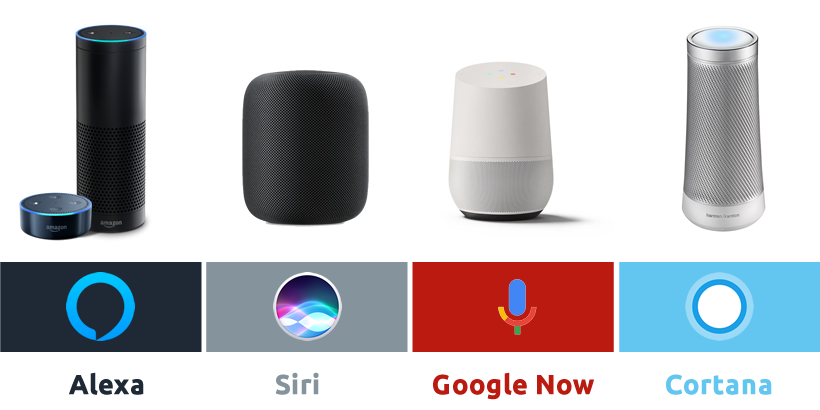
\includegraphics[scale=.45]{figures/voice-assistants-battle}}
        \caption{Smart Assistant, Sumber: https://blog.evolvemachinelearners.com/voice-assistant-its-history-twist-and-turn/}
		\label{assistant}
\end{figure}

\end{enumerate}

\subsection{Mendeteksi Deepfake Voice}
Karena teknologi suara terus meningkat, memiliki teknologi yang dapat mengenali dan menghentikan penggunaan ucapan palsu untuk penipuan dan penipuan sangat penting. 

Anti-spoofing suara, juga disebut deteksi keaktifan suara, adalah teknologi yang mampu membedakan antara suara langsung dan suara yang direkam, dimanipulasi, atau sintetis. Banyak pemalsuan saat ini tidak terlihat oleh telinga manusia, tetapi dapat dideteksi oleh perangkat lunak berbasis AI yang dilatih untuk mengidentifikasi artefak yang tidak ada dalam suara langsung. 

Teknologi yang mendeteksi perangkat lunak kloning suara AI pada awalnya dibuat untuk memecahkan masalah spoofing biometrik suara. Di mana biometrik suara mencocokkan suara seseorang dengan templat suara pada file, teknologi anti-spoofing memeriksa untuk memastikan suara itu hidup. Teknologi ini akan terus beradaptasi untuk mengatasi kasus penggunaan tambahan karena penipuan kloning suara menjadi lebih umum. Topik tersebut bahkan menjadi fokus lokakarya FTC baru -baru ini dengan peserta dari ID R\&D DARPA, University of Florida, MIT Sloan School of Management, dan program Defending Democracy dari Microsoft.



\chapter{Tacotron-2}
Tacotron 2 merupakan penelitian yang diteliti oleh Google pada bulan Desember 2016. Tacotron-2 merupakan implementasi jaringan saraf untuk Text-to-Speech Synthesis. Silahkan kunjungi website https://google.github.io/tacotron/publications/tacotron2/ ini apabila teman-teman penasaran dengan penelitian tersebut. Apabila teman-teman perhatikan dan mencoba mendengarkan sampel suara yang ada di website tersebut bukankah sangat mirip dengan suara asli manusia? Setelah mendengarkan sampel suara tersebut saya menjadi sangat tertarik dengan penelitian tentang Arsitektur Tacotron-2 ini dan mencari tahu serta menerapkan model tersebut dalam project pembuatan voice cloning berbahasa indonesia ini. Cara kerja sistem dijelaskan oleh Jonathan Shen dan Ruoming Pang, Software Engineers, Google Brain and Machine Perception Teams.

''Singkatnya cara kerjanya seperti ini: Kami menggunakan model urutan-ke-urutan yang dioptimalkan untuk TTS untuk memetakan urutan huruf ke urutan fitur yang mengkodekan audio. Fitur-fitur ini, spektogram audio 80-dimensi dengan bingkai yang dihitung setiap 12,5 milidetik, tidak hanya menangkap pengucapan kata-kata, tetapi juga berbagai seluk-beluk ucapan manusia, termasuk volume, kecepatan, dan intonasi. Akhirnya fitur ini diubah menjadi bentuk gelombang 24 kHz menggunakan arsitektur mirip WaveNet."

\begin{figure}[H]
        \centerline{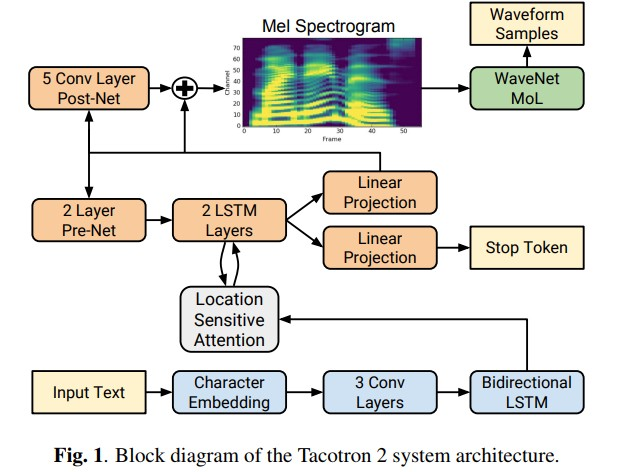
\includegraphics[scale=.75]{figures/fig1}}
        \caption{Blok Diagram dari Arsitektur Tacotron 2}
		\label{fig1}
\end{figure}

Bagian pertama dari model yaitu arsitektur Seq2Seq yang bertanggung jawab untuk mengubah teks menjadi mel-spektogram dan spektogram ini dimasukkan dalam model wave-net untuk menghasilkan bentuk gelombang audio. Satu hal yang menarik adalah kedua bagian dari arsitektur Tacotron (Seq2Seq dan vocoder Wavenet) ini dapat dilatih secara mandiri. Saya bekerja pada model Seq2Seq.
Modelnya adalah penyiapan enkoder-perhatian-dekoder di mana mereka menggunakan 'Perhatian sensitif lokasi'. Bagian pertama adalah Encoder yang mengubah urutan karakter menjadi vektor penyisipan kata. Representasi ini kemudian dikonsumsi oleh Decoder untuk memprediksi spektogram. Karena saya menggunakan dataset Indonesia, saya memastikan bahwa ruang karakter saya memiliki abjad Indonesia.

Encoder terdiri dari 3 lapisan konvolusi yang masing-masing berisi 512 filter berbentuk 5 x 1, diikuti oleh normalisasi batch dan aktivasi ReLU. Bagian selanjutnya adalah jaringan attention yang mengambil keluaran enkoder sebagai masukan dan mencoba meringkas urutan yang disandikan penuh sebagai vektor konteks dengan panjang yang tetap untuk setiap langkah keluaran dekoder.
Output dari lapisan konvolusi akhir dilewatkan ke lapisan LSTM dua arah tunggal yang berisi 512 unit (256 di setiap arah) untuk menghasilkan fitur yang dikodekan.

\section{MODEL BERBASIS PERHATIAN UNTUK PENGENALAN Pidato}
Mekanisme attention yang digunakan di sini memperhitungkan lokasi fokus pada langkah sebelumnya dan fitur urutan input.
Katakanlah kita memiliki data x = {x1,x2,x3….xN}. Kami meneruskan data ini ke encoder yang menghasilkan urutan keluaran yang dikodekan h = {h1,h2,h3….hN}.
A(i) = Perhatian( s(i-1), A(i-1), h ) di mana s(i-1) adalah status decoding sebelumnya dan A(i-1) adalah perataan sebelumnya.
s(i-1) adalah 0 untuk iterasi pertama dari langkah pertama.
Fungsi perhatian biasanya diimplementasikan dengan menilai setiap elemen dalam h secara terpisah dan kemudian menormalkan skor.
G(i) = A(i,0) h (0) + A(i,1) h (1) + ……. + A(i,N) h (N)
Y(i) ~ Hasilkan ( s(i-1), G(i) )
di mana s adalah output decoding, A(i) adalah vektor bobot perhatian yang disebut keselarasan.
Akhirnya, s(i) = Pengulangan ( s(i-1), G(i), Y(i) )
Pengulangan biasanya LSTM.

\subsection{Decoder}
Dekoder adalah jaringan saraf rekuren autoregresif yang memprediksi spektogram mel dari urutan input yang disandikan satu frame pada satu waktu. Prediksi dari langkah waktu sebelumnya pertama-tama dilewatkan melalui pra-net kecil yang berisi 2 lapisan yang terhubung penuh dari 256 unit ReLU tersembunyi. Output prenet dan vektor konteks perhatian digabungkan dan dilewatkan melalui tumpukan 2 lapisan LSTM uni-directional dengan 1024 unit. Akhirnya, spektogram mel yang diprediksi dilewatkan melalui post-net convolutional 5-lapisan yang memprediksi residu untuk ditambahkan ke prediksi untuk meningkatkan rekonstruksi keseluruhan. Setiap lapisan pasca jaring terdiri dari 512 filter dengan bentuk 5 × 1 dengan normalisasi batch, diikuti oleh aktivasi tanh pada semua kecuali lapisan terakhir.

\subsection{Loss Function}
Summed mean squared error (MSE)
Sejalan dengan prediksi bingkai spektogram, rangkaian keluaran LSTM dekoder dan konteks perhatian diproyeksikan ke skalar dan melewati aktivasi sigmoid untuk memprediksi kemungkinan bahwa urutan keluaran telah selesai. Prediksi "token berhenti" ini digunakan selama inferensi untuk memungkinkan model menentukan secara dinamis kapan harus menghentikan pembangkitan alih-alih selalu menghasilkan untuk durasi yang tetap.
Saya memutuskan untuk menggunakan pytorch untuk implementasi saya, melacak pelatihan dengan tensorboard , menggunakan GPU gcloud Tesla K80, terhubung ke port server dengan 'ssh -NfL', dan lab jupyter yang banyak digunakan selama pengembangan. [perlengkapan penyelamat hidup]
Saya mereferensikan berbagai repositori github [ 1 , 2 ] untuk memahami makalah, implementasi, mengoreksi bug dalam kode saya sendiri. Karena kompleksitas alami dari pernyataan masalah, saya tidak bisa mendapatkan hasil pidato yang menakjubkan seperti manusia tetapi saya belajar banyak hal tentang Text-to-speech dan itu adalah tujuan utama ketika saya mulai mengerjakan proyek ini.
Beberapa hasil untuk referensi:
\begin{figure}[H]
        \centerline{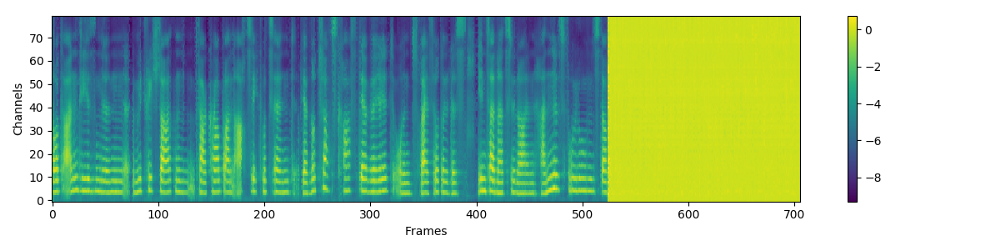
\includegraphics[scale=.75]{figures/ref1}}
        \caption{Spektogram mel yang diprediksi : Seperti yang dapat Anda bandingkan dengan wilayah atas, ia memiliki banyak celah dan masih membutuhkan banyak pelatihan. Sisi kanan (hijau solid) hanya padding dalam satu batch.}
		\label{ref1}
\end{figure}
\begin{figure}[H]
        \centerline{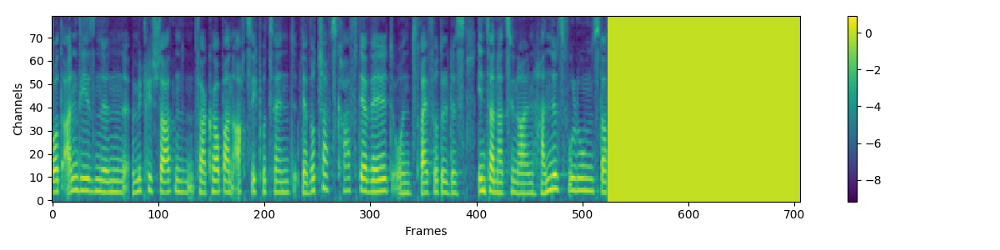
\includegraphics[scale=.75]{figures/ref2}}
        \caption{Target mel-spektogram}
		\label{ref2}
\end{figure}
\begin{figure}[H]
        \centerline{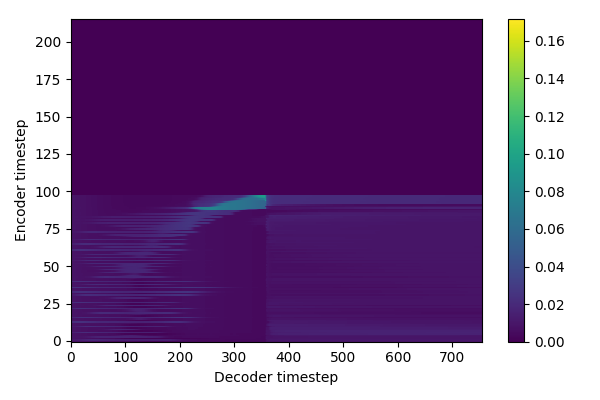
\includegraphics[scale=.75]{figures/ref3}}
        \caption{Perhatian (Seperti yang Anda lihat di sisi kiri bawah, sepertinya sedang belajar untuk menyelaraskan tetapi masih membutuhkan sekitar satu minggu pelatihan untuk mendapatkan diagonal yang sempurna untuk perhatian)}
		\label{ref3}
\end{figure}
Semua gambar yang dihasilkan di atas adalah setelah iterasi 50K (1 iterasi = 1 batch) yaitu 3 hari pelatihan. Model ini membutuhkan sekitar 300 ribu iterasi untuk mendekati seperti manusia. Anda dapat melihat bahwa, spektogram mel yang diprediksi terlihat cukup bagus bahkan ketika perhatian tidak dipelajari dengan benar. Selamatkan diri Anda dari jebakan dan pedulikan perhatian!

Menerapkan model dan pelatihan ternyata tidak sesepele yang saya kira awalnya. Saya menemukan banyak masalah yang saya ingin kalian ketahui sebelumnya dan menghemat waktu di GPU Anda.
Pelajari data Anda. Ini adalah bagian terpenting dari proyek. Dengarkan sampel data Anda, periksa panjang sampel teks, durasi sampel audio, dll. Anda dapat menghemat banyak waktu selama pelatihan, jika Anda mengetahui data Anda dengan baik. M-AILABS mengumumkan kumpulan data pidato besar mereka awal tahun ini. Mereka memiliki kumpulan data ucapan yang sangat banyak dalam berbagai bahasa. Saya menggunakan data Angela Merkel dari bagian wanita Jerman, yang memiliki 12 jam pidato dari pidato publik dan wawancaranya. Dataset ini lebih rendah dibandingkan dengan LJSpeech (dataset bahasa Inggris paling populer, 24 jam bicara). Saya menemukan ini hanya ketika saya mulai berlatih dan menghabiskan berhari-hari mengamati hasilnya. Jadi, bersiaplah!
TTS sangat mahal secara komputasi . Sebagai mahasiswa, saya baru saja memiliki akses ke satu GPU (Nvidia Tesla K80) di Google cloud. Mengingat struktur dataset yang saya gunakan, GPU saya hanya mengizinkan ukuran batch 8 saat pelatihan. Google mengatakan, mereka melatihnya dengan ukuran batch 64. Saya pertama kali mencoba dengan ukuran batch 2 (karena memori GPU terbatas) dan ketika model gagal menunjukkan konvergensi setelah 2-3 hari pelatihan, saya mengurutkan data saya sesuai panjang teks dan durasi audio, dan mulai berlatih dengan ukuran batch 8. Meskipun demikian, saya tidak dapat mengoptimalkan lebih banyak dengan dataset dan GPU yang saya miliki. Jadi, rencanakan dengan tepat.
Rasio pemaksaan guru. Dalam pelatihan paksa guru, model dibantu oleh label yang benar yaitu menggunakan kerangka Kebenaran Dasar saat ini untuk memprediksi langkah decoding berikutnya. Tidak jelas dalam makalah tentang rasio apa yang digunakan. Bahkan jika perhatiannya tidak dipelajari, model akan memprediksi kerangka yang baik untuk data pelatihan dalam mode paksaan guru tetapi dalam mode evaluasi itu tidak akan berhasil karena kita tidak memiliki kebenaran dasar (Mengira model itu bekerja sejak prediksi mels tampak bagus terlepas dari keberpihakan yang buruk). Saya melakukan pelatihan dengan 1.0, 0.75 dan 0.5 untuk membuat model belajar keberpihakan. Selama mode evaluasi, pemaksaan guru harus dimatikan.
Dibutuhkan berhari-hari untuk melatih dan mendapatkan keberpihakan. Ini adalah proses yang sangat rumit untuk melatih sistem TTS. Mungkin perlu sekitar 7–10 hari untuk melatih model asalkan Anda memiliki dukungan GPU terbatas (Kami bukan Google). Dan kemudian, men-debug kode dengan model seperti itu, adalah cerita lain.
Tuning hyperparameter adalah bagian yang sangat penting dari sistem Tacotron-2. Ukuran batch, tingkat pembelajaran, rasio guru-memaksa, panjang batch adalah beberapa parameter yang harus Anda perhatikan juga. Hal-hal bervariasi dengan dataset, jadi sangat sensitif!

Text-to-speech masih merupakan masalah penelitian yang sangat kompleks dan sangat menarik untuk dikerjakan. Pengalaman saya secara keseluruhan luar biasa dan saya belajar banyak hal tentang sistem TTS, bentuk gelombang audio, jaringan berulang, mel-spektogram, mekanisme perhatian dan saya harap posting ini dapat membantu Anda dalam perjalanan Anda dengan sistem TTS. Di masa mendatang, saya ingin melihat versi model Tacotron-2 yang dioptimalkan, sesuatu yang lebih kuat di berbagai bahasa, lebih mudah dilatih, dan tidak terlalu berat secara komputasi.
Jadi, saya hanya akan mengatakan, praproses data Anda dengan baik, sesuaikan hyperparameter Anda, catat semuanya di tensorboard dan mulai! Semua yang terbaik!

\chapter{WaveNet}
\section{Speech Synthesis}
Di berbagai media, Anda mungkin pernah menyaksikan Stephen Hawking berbicara di depan mahasiswanya. Fisikawan yang terkenal dengan teori black hole-nya ini sudah tidak mampu lagi mengeluarkan suara dari lisannya, namun berkat teknologi speech synthesizer, dia masih bisa bercakap-cakap. Mesin speech synthesizer Hawking memang cukup kompleks. Alat ini tidak hanya memproduksi suara, tetapi juga menangkap input dari gerakan mata sang doktor. Demikian pula, misalnya, dengan aplikasi voice command yang banyak tertanam di smartphone mutakhir yang memadukan speech recognizer dengan speech synthesizer.

Aplikasi speech synthesizer yang paling sederhana sebenarnya ada pada setiap PC ber-OS Windows. Bila anda menekan tuts Winkey + U di keyboard, Windows akan mengaktifkan Utility Manager, yang di dalamnya terdapat aplikasi Microsoft Narrator. Aplikasi ini akan membaca setiap jendela yang anda aktifkan, termasuk tombol-tombol di dalamnya. Atau, mungkin anda pernah menginstal aplikasi microsoft reader di PC. Aplikasi yang diperuntukkan bagi file >LTT ini pun dilengkapi dengan kemampuan menerjemahkan teks menjadi suara (text to speech) yang merupakan contoh teknologi speech synthesizer.

\begin{figure}[H]
        \centerline{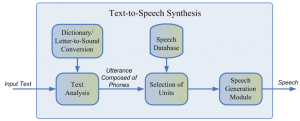
\includegraphics[scale=.75]{figures/speech}}
        \caption{Speech Synthesis}
		\label{speech}
\end{figure}

Speech synthesis adalah sebuah kemampuan bicara manusia yang dibuat oleh manusia (artificial). Sebuah sistem komputer digunakan untuk tujuan ini yang disebut sebagai speech synthesizer, dan dapat diimplementasikan ke dalam software atau hardware. Sebagai contoh sebuah sistem text-to-speech (TTS) yang dapat mengkonversikan teks dengan bahasa biasa menjadi suara.

Sebuah sistem komputer yang digunakan untuk tujuan ini disebut speech synthesizer, dan dapat diimplementasikan dalam perangkat lunak atau perangkat keras produk. Sebuah teks-to-speech (TTS) sistem mengkonversi teks bahasa normal menjadi berbicara; sistem lain membuat representasi linguistik simbolik seperti transkripsi fonetik ke dalam pidato, pidato disintesis dapat dibuat dengan menggabungkan potongan pidato direkam yang disimpan dalam database. Sistem berbeda dalam ukuran unit pidato disimpan, sebuah sistem yang menyimpan telepon atau diphones menyediakan berbagai keluaran terbesar, tapi mungkin kurang jelas.

Speech synthesis adalah transformasi dari teks ke arah suara (speech). Transformasi ini mengkonversi teks ke pemadu suara (speech synthesis) yang sebisa mungkin dibuat menyerupai suara nyata, disesuaikan dengan aturan – aturan pengucapan bahasa.TTS (text to speech) dimaksudkan untuk membaca teks elektronik dalam bentuk buku, dan juga untuk menyuarakan teks dengan menggunakan pemaduan suara. Sistem ini dapat digunakan sebagai sistem komunikasi, pada sistem informasi referral, dapat diterapkan untuk membantu orang-orang yang kehilangan kemampuan melihat dan membaca.

Synthesized speech dapat diciptakan dengan menggabungkan beberapa potongan-potongan dari pembicaraan/pidato yang sudah direkam dalam sebuah basis data. Kualitas dari sebuah speech synthesizer dilihat dari kemiripannya dengan suara manusia dan kemampuannya untuk bisa dipahami. Program TTS yang jelas dapat membantu orang dengan gangguan visual atau ketidakmampuan membaca, untuk mendengarkan pada pekerjaan yang tertulis dalam komputer. Banyak Sistem Operasi komputer yang telah dimasukkan speech synthesizer sejak tahun 1980-an.

Sebuah sistem text-to-speech (atau “mesin”) terdiri dari dua bagian: front-end dan back-end . Front-end memiliki dua tugas utama. Pertama, mengubah teks mentah berisi simbol seperti angka dan singkatan menjadi setara dengan kata-kata tertulis-out. Proses ini sering disebut normalisasi teks, pra-pengolahan, atau tokenization . Front-end kemudian memberikan transkripsi fonetik untuk setiap kata, dan membagi dan menandai teks ke unit prosodi , seperti frase , klausa , dan kalimat . Proses menetapkan transkripsi fonetik untuk kata-kata ini disebut teks-ke-fonem atau grafem konversi -untuk-fonem. Transkripsi fonetik dan informasi prosodi bersama-sama membentuk representasi linguistik simbolik yang output dengan front-end. Back-end-sering disebut sebagai synthesizer-maka mengubah representasi linguistik simbolik menjadi suara. Dalam sistem tertentu, bagian ini meliputi perhitungan dari target prosodi (kontur pitch, durasi fonem), yang kemudian dikenakan pada pidato output.

\subsection{Sejarah Speech Synthesis}
Upaya yang paling awal untuk menghasilkan lahirnya pemandu suara, pada abad XVIII. Terlepas dari kenyataan bahwa upaya pertama  adalah bentuk mesin mekanis, kita dapat mengatakan hari ini  bahwa synthesizer sudah berkualitas tinggi. Pada tahun 1779 di

St Petersburg, Rusia Profesor Kratzenshtein Kristen  fisiologis menjelaskan perbedaan antara lima vokal panjang  (/ A /, / e /, / i /, / o /, dan / u /) dan membuat alat untuk menghasilkan  mereka artifisial. Tahun 1791 di Wina, Wolfgang von Kempelen memperkenalkan nya “Akustik-Mekanik Mesin Speech”. Dalam  sekitar pertengahan 1800-an Charles Wheatstone dibangun terkenal  versi mesin berbicara von Kempelen’s.

Generasi dari sistem pemaduan suara ini dapat dibagi ke dalam 3 masa, yaitu:

\begin{enumerate}
\item Generasi pertama (1962-1977). Format sintesis dari fonem adalah teknologi dominan. Teknologi ini memanfaatkan aturan berdasarkan penguraian fonetik pada kalimat untuk kontur frekuensi forman. Beberapa sintesis masih miskin atau kurang dalam kejelasan dan kealamiannya.
\item Generasi kedua (1977-1992). Metode pemadu suara adalah diphone diwakilkan  dengan parameter LPC. Hal tersebut menunujukkan bahwa kejelasan yang baik pada pemadu suara dapat diperoleh dengan andal dari input teks dengan menggabungkan diphone yang sesuai dengan unit. Kejelasan meningkat selama sintesis forman, tetapi kealamian dari pemadu suara masih tetap rendah.
\item Generasi ketiga (1992-sekarang). Generasi ini ditandai dengan metode ‘ sintesis pemilihan unit’ yang diperkenalkan dan disempurnakan oelh Sagisaka di Labs ATR Kyoto. Hasil dari pemandu suara pada periode ini sangat mendekati human-generated speech pada bagian kejelasan dan kealamian.
\end{enumerate}

Teknologi pemadu suara modern melibatkan metode dan algoritma yang canggih dan rumit. alat pemadu suara  dari keluarga “Infovox” mungkin mejadi salah satu multi bahasa TTS yang paling dikenal saat ini. Versi komersial pertamanya, Infovox-SA 101, dikembangkan pada tahun 1982 di Institute Teknologi Royal, Swedia dan didasarkan pada sintesis forman.

AT \& T Bell Laboratories (Lucent Technologies) juga memiliki tradisi yang sangat panjang tentang pemandu suara (speech synthesis). TTS lengkap yang pertama didemostrasikan di Boston pada tahun 1972 dan diliris pada tahun 1973. Hal ini didasarkan pada model artikulatoris yang sikembangkan oleh Ceceil Coker (Klatt 1987). Pengembangan proses dari sistem penggabungan sintesis ini dimulai oleh Joseph Olive pada pertengahan tahun 1970-an (Bell Labs 1997). Sistem ini sekarang sudah tersedia untuk bahasa Inggris, Perancis, Spanyol, Italia, Jerman, Rusia, Rumania, Cina, dan Jepang (Mcbius et al 1996).

\subsection{Perangkat Speech Synthesis}
Pidato sistem sintesis berbasis komputer pertama diciptakan pada akhir 1950-an. Pertama umum Inggris sistem text-to-speech dikembangkan oleh Noriko Umeda et al. Pada tahun 1968 di Laboratorium Elektroteknik, Jepang. Pada tahun 1961, fisikawan John Larry Kelly, Jr dan Louis rekan Gerstman menggunakan IBM 704 komputer untuk mensintesis pidato, acara yang paling menonjol dalam sejarah Bell Labs . Kelly perekam suara synthesizer ( vocoder ) ulang lagu ” Daisy Bell “, dengan iringan musik dari Max Mathews .Kebetulan, Arthur C. Clarke mengunjungi teman dan kolega John Pierce di fasilitas Bell Labs Murray Hill. Clarke begitu terkesan oleh demonstrasi bahwa ia digunakan dalam adegan klimaks dari skenario-Nya untuk novel nya 2001: A Space Odyssey, di mana HAL 9000 komputer menyanyikan lagu yang sama seperti yang sedang ditidurkan oleh astronot Dave Bowman. Meskipun keberhasilan pidato sintesis murni elektronik, penelitian masih terus dilakukan ke synthesizer pidato mekanis.

Handheld elektronik menampilkan sintesis pidato mulai muncul pada 1970-an. Salah satu yang pertama adalah Telesensory Systems Inc(TSI) Pidato + kalkulator portabel untuk orang buta pada tahun 1976. Perangkat lain yang diproduksi terutama untuk tujuan pendidikan, seperti Bicara \& Eja , yang diproduksi oleh Texas Instruments pada tahun 1978. Fidelity merilis versi berbicara komputer catur elektronik pada tahun 1979. Yang pertama video game yang memiliki fitur sintesis pidato adalah 1.980 shoot ’em up arcade game , Stratovox , dari Sun Electronics. Contoh lain awal adalah versi arcade dari Berzerk , dirilis pada tahun yang sama.Pertama multi-player permainan elektronik menggunakan sintesis suara adalah Milton dari Milton Bradley Company , yang memproduksi perangkat di tahun 1980.

\subsection{Teknologi Speech Synthesis}
Yang paling penting dalam kualitas sistem speech synthesis adalah kealamian dan kejelasannya. Kealamaian menjelaskan bagaimana dekatnya suara output dengan suara manusia, sementara kejelasan adalah dengan kemudahan di mana output tersebut dapat dipahami. Speech synthesizer yang ideal adalah yang alami dan jelas. Sistem speech synthesis biasanya mencoba untuk memaksimalkan kedua karakteristik.

Kualitas terpenting dari sebuah aplikasi speech synthesizer adalah seberapa alami dan inteligibel output yang dihasilkannya. Alami, artinya seberapa dekat suara yang dihasilkan aplikasi speech synthesizer dengan suara manusia. Sedangkan inteligibel adalah seberapa mudah output tersebut dipahami oleh manusia. Semua aplikasi speech synthesizer berusaha untuk menghasilkan output yang alami dan inteligibel sekaligus.

Sampai saat ini, ada banyak teknologi untuk meng-generate gelombang suara sintetis ini. Dua teknologi yang paling banyak digunakan adalah concatenative synthesis dan formant synthesis. Keduanya memiliki keunggulan dan kekurangan sendiri-sendiri.

Teknologi pertama, concatenative synthesis, berbasis pada rangkaian (atau merangkai bersama) segmen-segmen dari suara yang direkam. Umumnya, teknologi ini menghasilkan suara sintesis yang terdengar paling alami.Namun, perbedaan antara suara alami yang direkam dengan segmentasi gelombang bunyi kadang menghasilkan suara yang menggangu. Mirip seperti suara pemberitahuan nomor antrean di bank atau suara call center operator ponsel yang menyebutkan sisa pulsa dan masa berlaku kartu ponsel anda.

Teknologi kedua, formant synthesis, tidak menggunakan sampel suara manusia melainkan membuat suara sintesi menggunakan model akustik. Parameter-parameter seperti frekuensi dasar, alunan suara, dan tingkat kebisingan bervariasi dari waktu ke waktu untuk menciptakan gelombang suara buatan.

Kebanyakan aplikasi berbasis teknologi ini menghasilkan suara buatan (tidak alami) seperti suara robot. Melihat keterbatasan kedua teknologi ini dalam menghasilkan suara buatan, seperti kita harus sabar menunggu pengembangannya lebih lanjut dalam beberapa tahun atau dekade ke depan.

Kualitas yang paling penting dari sebuah sistem sintesis pidato kewajaran dan dimengerti. kealamian menjelaskan seberapa dekat output terdengar seperti suara manusia, sementara kejelasan adalah kemudahan yang output dipahami. Speech synthesizer yang ideal adalah baik alam dan dimengerti. Sistem sintesis pidato biasanya mencoba untuk memaksimalkan kedua karakteristik.

Dua teknologi utama dalam pembuatan gelombang suara synthetic speech adalah Concatenative Synthesis dan Formant Synthesis. Setiap teknologi mempunyai kekuatan dan kelemahannya, dan penggunaan yang ditujukan dari sistem synthesis akan menentukkan pendekatan mana yang digunakan.

\begin{enumerate}
\item Concatenative Synthesis
Concantenative synthesis didasarkan dengan penggabungan dari segmen-segmen dari pembicaraan yang sudah direkam. Secara umum, concatenative synthesis memproduksi synthesized speech dengan suara yang paling alami. Tetapi, perbedaan antara variasi alami dalam pembicaraaan dan sifat dari teknik otomasi untuk pensegmentasian gelombang suara terkadang menghasilkan kesalahan suara dalam output. Namun, perbedaan antara variasi alami dalam pidato dan sifat teknik otomatis untuk membagi bentuk gelombang kadang-kadang menyebabkan gangguan terdengar pada output. Ada tiga sub-jenis utama dari sintesis concatenative.
\begin{enumerate}
\item Sintesis Pemilihan unit
Sintesis Pemilihan unit menggunakan besar database pidato direkam. Selama pembuatan database, setiap ucapan tercatat tersegmentasi ke dalam beberapa atau semua hal berikut: individu telepon , diphones , setengah-telepon, suku kata , morfem , kata , frase , dan kalimat . Biasanya, pembagian ke dalam segmen dilakukan dengan menggunakan dimodifikasi khusus recognizer pidato disetel ke “keselarasan dipaksa” mode dengan beberapa koreksi manual setelah itu, dengan menggunakan representasi visual seperti yang gelombang dan spektogram .  Sebuah indeks unit dalam database pidato kemudian dibuat berdasarkan segmentasi dan parameter akustik seperti frekuensi dasar (lapangan ), durasi, posisi dalam suku kata, dan telepon tetangga. Pada waktu berjalan , target ucapan yang diinginkan dibuat dengan menentukan rantai terbaik unit calon dari database (pemilihan unit). Proses ini biasanya dicapai dengan menggunakan khusus tertimbang pohon keputusan.

Pemilihan unit menyediakan kealamian terbesar, karena hanya berlaku sedikit pemrosesan sinyal digital (DSP) untuk pidato direkam. DSP sering membuat pidato yang direkam terdengar kurang alami, meskipun beberapa sistem menggunakan sejumlah kecil pengolahan sinyal pada titik Rangkaian untuk menghaluskan bentuk gelombang. Output dari yang terbaik unit-seleksi sistem sering dibedakan dari suara manusia nyata, terutama dalam konteks dimana sistem TTS telah disetel. Namun, kealamian maksimum biasanya membutuhkan unit-pilihan database pidato menjadi sangat besar, dalam beberapa sistem mulai ke gigabyte data dicatat, mewakili puluhan jam berbicara.  Juga, pilihan algoritma Unit telah dikenal untuk memilih segmen dari Tempat yang menghasilkan kurang dari sintesis ideal (misalnya kata-kata kecil menjadi tidak jelas) bahkan ketika pilihan yang lebih baik ada dalam database. Baru-baru ini, peneliti telah mengusulkan berbagai metode otomatis untuk mendeteksi segmen alami di unit-pilihan sistem sintesis pidato.
\item Sintesis diphone
Sintesis diphone menggunakan database pidato minimal berisi semua diphones (suara-to-suara transisi) yang terjadi dalam suatu bahasa. Jumlah diphones tergantung pada fonotaktik bahasa: misalnya, Spanyol memiliki sekitar 800 diphones, dan Jerman sekitar 2500. Dalam sintesis diphone, hanya satu contoh dari setiap diphone terkandung dalam database pidato. Pada saat runtime, target prosodi kalimat ditumpangkan pada unit-unit minimal dengan cara pemrosesan sinyal digital teknik seperti linear predictive coding ,PSOLA atau MBROLA. Diphone sintesis menderita gangguan sonik sintesis concatenative dan robot-terdengar sifat sintesis forman, dan memiliki beberapa keuntungan baik pendekatan lain dari ukuran kecil. Dengan demikian, penggunaannya dalam aplikasi komersial menurun, meskipun terus digunakan dalam penelitian karena ada beberapa implementasi perangkat lunak tersedia secara bebas.
\item Domain-spesifik sintesis
Domain-spesifik sintesis concatenates direkam sebelumnya kata dan frase untuk menciptakan ucapan-ucapan yang lengkap. Hal ini digunakan dalam aplikasi di mana berbagai teks output sistem akan terbatas pada domain tertentu, seperti jadwal angkutan pengumuman atau laporan cuaca.  Teknologi ini sangat sederhana untuk menerapkan, dan telah digunakan secara komersial untuk waktu yang lama , dalam perangkat seperti berbicara jam dan kalkulator. Tingkat kealamian sistem ini bisa sangat tinggi karena berbagai jenis kalimat terbatas, dan mereka cocok dengan prosodi dan intonasi dari rekaman asli.

Karena sistem ini dibatasi oleh kata-kata dan frasa dalam database mereka, mereka tidak tujuan umum dan hanya dapat mensintesis kombinasi kata dan frase yang mereka telah terprogram. Campuran kata-kata dalam bahasa alami diucapkan namun masih dapat menyebabkan masalah kecuali banyak variasi diperhitungkan. Misalnya, dalam non-rhotic dialek dari bahasa Inggris “r” dalam kata-kata seperti “jelas” biasanya hanya diucapkan ketika kata berikut memiliki vokal sebagai huruf pertama (misalnya”membersihkan” direalisasikan sebagai  ). Demikian juga di Perancis , banyak konsonan akhir menjadi tidak lagi diam jika diikuti oleh sebuah kata yang dimulai dengan vokal, efek yang disebut penghubung . Ini pergantian tidak bisa direproduksi oleh sistem kata-Rangkaian sederhana, yang akan membutuhkan kompleksitas tambahan untuk konteks-sensitif .
\end{enumerate}
\item Formant Synthesis
Formant synthesis tidak menggunakan pembicaraan manusia sebagai sample pada runtime. Daripada itu, synthesized speech yang dihasilkan dibuat dengan additive synthesis dan sebuah model akustik (physical modelling synthesis).

Parameter seperti frekuensi dasar, penyuaraan, dan tingkat kebisingan di variasikan dari waktu ke waktu untuk menciptakan gelombang buatan (artificial) dari sebuah pembicaraan. Banyak sistem yang berdasarkan formant synthesis menciptakan pembicaraan yang seperti robot yang tidak mungkin dapat dikenal sebagai suara manusia. Tetapi, kealamian maksimum bukan selalu tujuan dari sebuah sistem speech synthesis, dan sistem formant synthesis mempunyai keuntungan dari sistem concatenative. Pembicaraan yang di-formant synthesis-kan dapat menjadi sangat jelas, bahkan dalam kecepatan yang tinggi, sehingga menghindari kesalahan suara yang sering dialami sistem concatenative.

Formant synthesis biasanya program yang lebih kecil dari concatenative sistem karena ia tidak menggunakan basis data dari sampel-sampel pembicaraan. Oleh karena itu formant synthesis dapat ditanamkan dalam sistem yang mempunyai memory dan microprosesor yang terbatas. Karena sistem yang berdasarkan formant mempunyai kendali penuh dari sluruh aspek dari hasil pembicaraan, variasi yang luas dari prosodi dan intonasi dapat dihasilkan, menyampaikan tidak hanya pertanyaan dan pernyataan tetapi juga emosi dan nada suara.

Formant sintesis tidak menggunakan sampel suara manusia pada saat runtime. Sebaliknya, keluaran suara yang disintesis dibuat menggunakan aditif sintesis dan model akustik (sintesis pemodelan fisik ). Parameter seperti frekuensi dasar , menyuarakan , dan kebisingan tingkat yang bervariasi dari waktu ke waktu untuk membuat gelombang pidato buatan. Metode ini kadang-kadang disebut aturan berbasis sintesis; Namun, banyak sistem concatenative juga memiliki aturan berbasis komponen. Banyak sistem yang didasarkan pada teknologi sintesis forman menghasilkan buatan, robot yang terdengar pidato yang tidak akan pernah salah untuk pidato manusia. Namun, kealamian maksimum tidak selalu tujuan sistem sintesis pidato, dan sistem sintesis forman memiliki keunggulan dibandingkan sistem concatenative. Pidato forman-disintesis dapat diandalkan dimengerti, bahkan pada kecepatan yang sangat tinggi, menghindari Glitches akustik yang biasanya wabah sistem concatenative. Kecepatan tinggi disintesis pidato digunakan oleh tunanetra untuk navigasi cepat komputer menggunakan pembaca layar . Synthesizer forman adalah program biasanya lebih kecil dibandingkan dengan sistem concatenative karena mereka tidak memiliki database contoh pidato. Karena itu mereka dapat digunakan dalam embedded system , di mana memori dan mikroprosesor daya terutama terbatas. Karena sistem berbasis forman memiliki kontrol penuh dari semua aspek pidato output, berbagai prosodies dan intonasi dapat menjadi output, tidak hanya menyampaikan pertanyaan dan pernyataan, tetapi berbagai emosi dan nada suara.

Contoh non-real-time tapi sangat akurat kontrol intonasi dalam sintesis forman meliputi pekerjaan yang dilakukan pada akhir tahun 1970 untuk Texas Instruments mainan Bicara \& Eja , dan pada awal tahun 1980 Sega arcade mesin dan dalam banyak Atari, Inc. game arcade menggunakan TMS5220 LPC Chips . Menciptakan intonasi yang tepat untuk proyek ini adalah telaten, dan hasilnya masih harus dicocokkan dengan real-time text-to-speech interface.
\item Sintesis artikulatoris
Sintesis artikulatoris mengacu pada teknik komputasi untuk sintesis pidato berdasarkan model manusia saluran vokal dan artikulasi proses yang terjadi di sana. Synthesizer artikulatoris pertama teratur digunakan untuk percobaan laboratorium dikembangkan di Haskins Laboratories di pertengahan 1970-an oleh Philip Rubin, Tom Baer, dan Paul Mermelstein. Synthesizer ini, yang dikenal sebagai ASY, didasarkan pada model saluran vokal dikembangkan di Bell Laboratories pada tahun 1960 dan 1970-an oleh Paul Mermelstein, Cecil Coker, dan rekan.

Sampai saat ini, model sintesis artikulatoris belum dimasukkan ke dalam sistem sintesis pidato komersial. Sebuah pengecualian adalah NeXT sistem berbasis awalnya dikembangkan dan dipasarkan oleh Trillium Suara Research, sebuah perusahaan spin-off dari University of Calgary , di mana banyak riset asli dilakukan. Setelah runtuhnya berbagai inkarnasi NeXT (dimulai oleh Steve Jobs pada akhir tahun 1980 dan bergabung dengan Apple Computer pada tahun 1997), perangkat lunak TRILLIUM diterbitkan di bawah GNU General Public License , dengan bekerja terus sebagai gnuspeech . Sistem, pertama kali dipasarkan pada tahun 1994, memberikan penuh text-to-speech konversi berbasis artikulatoris menggunakan Waveguide atau transmisi-line analog dari saluran mulut dan hidung manusia dikendalikan oleh Carré ini “model daerah khas”.
\item Sintesis berbasis HMM
Sintesis berbasis HMM  adalah metode sintesis berdasarkan model Markov tersembunyi , juga disebut statistik Parametrik Sintesis. Dalam sistem ini, spektrum frekuensi ( vokal ),frekuensi dasar (sumber vokal), dan durasi ( prosodi ) berbicara dimodelkan secara bersamaan oleh HMMs. Pidato bentuk gelombang yang dihasilkan dari HMMs sendiri berdasarkan maksimum kriteria.
\item Sintesis Sinewave
Sintesis sinewave adalah teknik untuk sintesis pidato dengan mengganti forman (band utama energi) dengan peluit nada murni.

Ada beberapa masalah yang terdapat pada pemaduan suara, yaitu:
\begin{enumerate}
\item User sangat sensitif terhadap variasi dan informasi suara. Oleh sebab itu, mereka tidak dapat memberikan toleransi atas ketidaksempurnaan pemadu suara.
\item Output dalam bentuk suara tidak dapat diulang atau dicari dengan mudah.
\item Meningkatkan keberisikan pada lingkungan kantor atau jika menggunakan handphone, maka akan meningkatkan biaya pengeluaran.
\end{enumerate}
\end{enumerate}


\chapter{Single-Speaker Voice Cloning}
\section{Model SV2TTS}
Model Speech Vector to TTS (SV2TTS) terdiri dari tiga bagian, masing-masing dilatih secara individual.
Hal ini memungkinkan setiap bagian dilatih pada data independen, sehingga mengurangi kebutuhan untuk mendapatkan data multispeaker berkualitas tinggi.

\begin{figure}[H]
        \centerline{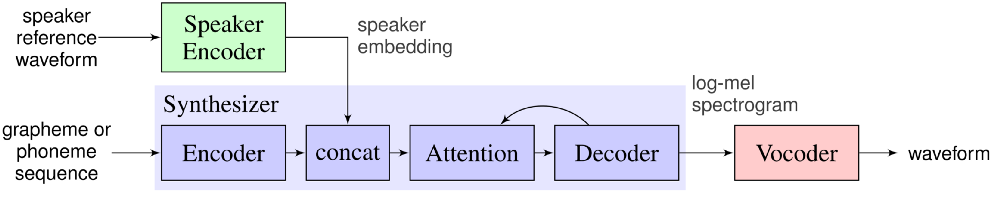
\includegraphics[scale=.35]{figures/arsitektur}}
        \caption{Arsitektur SV2TTS umum Sumber: Jia, Zhang, dan Weiss et al.}
		\label{arsitektur}
\end{figure}

\subsection{Speaker Encoder}

Bagian pertama dari model SV2TTS adalah encoder speaker.
Tugas speaker encoder adalah mengambil beberapa input audio (dikodekan sebagai bingkai spektogram mel), dari speaker tertentu, dan mengeluarkan embedding yang menangkap "bagaimana suara speaker". Encoder pembicara tidak peduli dengan kata-kata yang diucapkan pembicara, atau tentang kebisingan di latar belakang, yang dia pedulikan hanyalah suara pembicara, misalnya, suara bernada tinggi/rendah, aksen, nada, dll. Semua fitur ini digabungkan menjadi vektor berdimensi rendah, yang secara formal dikenal sebagai vektor-d, atau secara informal sebagai penyematan speaker. Akibatnya, ujaran yang diucapkan oleh penutur yang sama akan saling berdekatan pada penyematan penutur, sedangkan tuturan yang diucapkan oleh penutur yang berbeda akan berjauhan pada penyematan penutur\cite{8999436, DBLP:journals/corr/HeigoldMBS15}.
\begin{figure}[H]
        \centerline{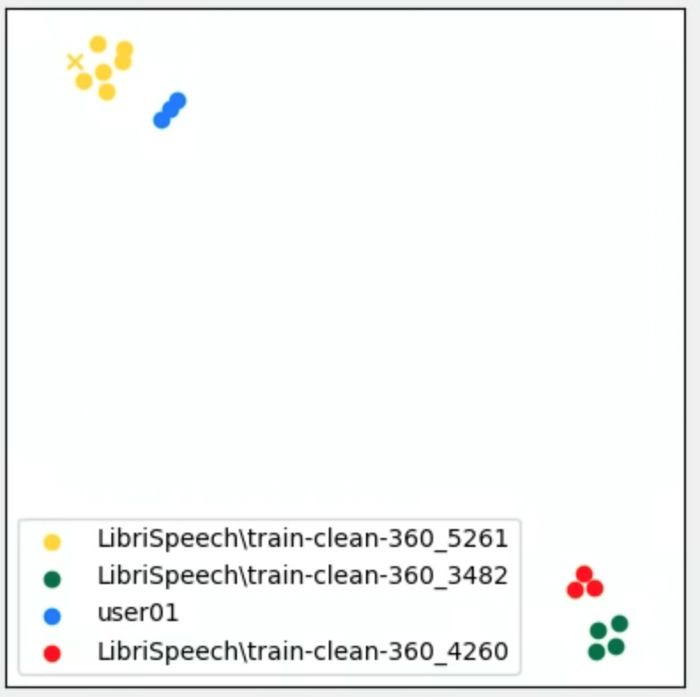
\includegraphics[scale=.35]{figures/encoder}}
        \caption{Representasi visual dari embeddings, setiap warna adalah speaker yang berbeda\cite{DBLP:journals/corr/abs-1806-04558}}
		\label{encoder}
\end{figure}

Untuk belajar menghasilkan embeddings ini, penulis menjelaskan proses berikut:
\begin{enumerate}
\item Pertama, contoh audio ucapan disegmentasi menjadi klip 1,6 detik tanpa transkrip dan diubah menjadi spektogram mel.
\item Kemudian speaker encoder dilatih untuk mengambil dua sampel audio dan memutuskan apakah speaker yang sama memproduksinya atau tidak. Sebagai produk sampingan, ini memaksa encoder speaker untuk membuat embeddings yang mewakili suara speaker.
\end{enumerate}
Proses pelatihan mirip dengan jaringan saraf siam jika Anda sudah familiar dengan mereka.

\subsection{Synthesizer}
Synthesizer adalah bagian dari SV2TTS yang menganalisis input teks untuk membuat spektogram mel, yang kemudian diubah oleh vocoder menjadi suara.
Synthesizer mengambil urutan teks — dipetakan ke fonem (unit terkecil dari suara manusia, misalnya, suara yang Anda buat saat mengucapkan 'a'), bersama dengan embeddings yang dihasilkan oleh encoder speaker, dan menggunakan arsitektur Tacotron 2 untuk menghasilkan bingkai dari spektogram mel secara berulang
\begin{figure}[H]
        \centerline{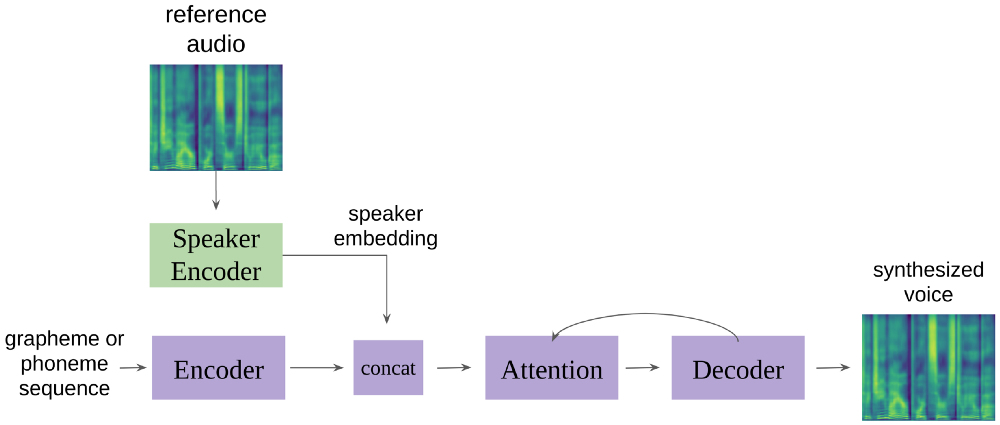
\includegraphics[scale=.35]{figures/model}}
        \caption{Model Arsitektur Multi-Speaker Voice Cloning \cite{DBLP:journals/corr/abs-1806-04558}}
		\label{model}
\end{figure}

Berikut Proses Training Synthesizer:

\begin{enumerate}
\item Pertama, kami mengumpulkan urutan fonem dan spektogram mel dari pembicara yang mengucapkan kalimat itu.
\item Kemudian, spektogram mel diteruskan ke encoder speaker untuk menghasilkan embedding speaker.
\item Selanjutnya, pembuat enkode penyintesis menggabungkan penyandian urutan fonemnya dengan penyematan speaker.
\item Spektogram mel dihasilkan secara berulang oleh decoder dan bagian perhatian dari synthesizer
\item Terakhir, spektogram mel dibandingkan dengan target awal untuk menghasilkan kerugian, yang kemudian dioptimalkan
\end{enumerate}

\begin{figure}[H]
        \centerline{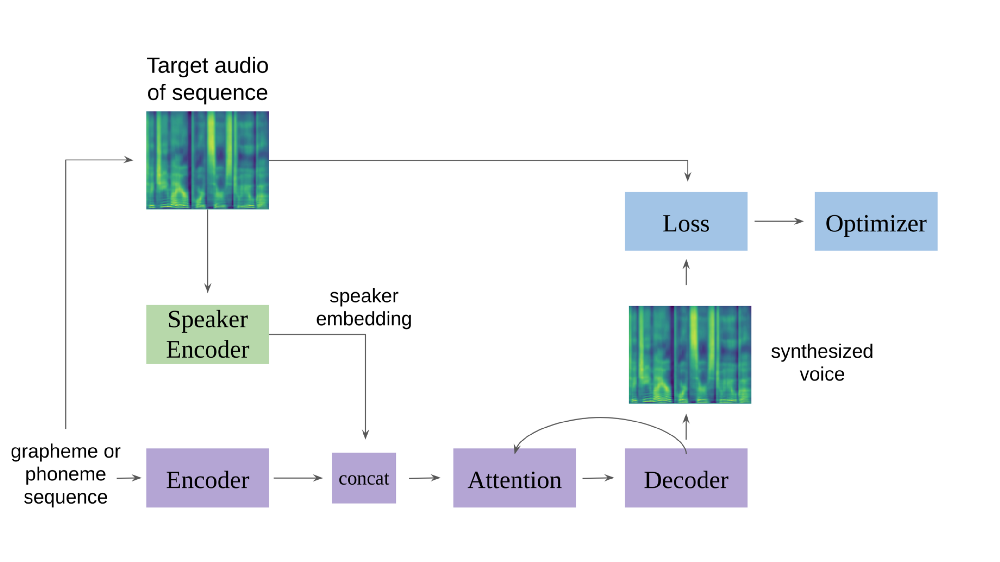
\includegraphics[scale=.35]{figures/train}}
        \caption{Training Synthesizer\cite{DBLP:journals/corr/abs-1806-04558}}
		\label{train}
\end{figure}

\subsection{Vocoder}
Pada titik ini, synthesizer telah membuat spektogram mel, tetapi kami masih belum dapat mendengarkan apa pun. Untuk mengubah spektogram mel menjadi gelombang audio mentah, penulis menggunakan vocoder.
Vocoder khusus yang digunakan di sini didasarkan pada model WaveNet DeepMind , yang menghasilkan bentuk gelombang audio mentah dari teks, dan pada satu titik canggih untuk sistem TTS\cite{DBLP:journals/corr/OordDZSVGKSK16}.
\begin{figure}[H]
        \centerline{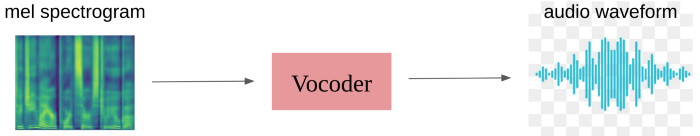
\includegraphics[scale=.35]{figures/vocoder}}
        \caption{Vocoder\cite{DBLP:journals/corr/abs-1806-04558}}
		\label{vocoder}
\end{figure}


\subsection{Alur Model SV2TTS}
berikut adalah alur modelnya:
\begin{enumerate}
\item Encoder speaker mendengarkan sampel audio yang diberikan dan menghasilkan embedding
\item Synthesizer mengambil daftar fonem dan penyematan speaker, kemudian menghasilkan spektogram mel
\item Vocoder saraf menguraikan spektogram mel menjadi bentuk gelombang audio yang dapat kita dengarkan
\end{enumerate}

\subsection{Mengukur Kualitas Hasil}
Penulis menggunakan penilai manusia untuk mengukur kealamian dan kesamaan ucapan yang dihasilkan model.
Kealamian mengukur seberapa "manusia" ucapan itu terdengar, sementara kesamaan mengukur seberapa mirip suara pidato yang disintesis dengan pembicara aslinya.
Penilai berinteraksi melalui GUI yang terlihat seperti:
\begin{figure}[H]
        \centerline{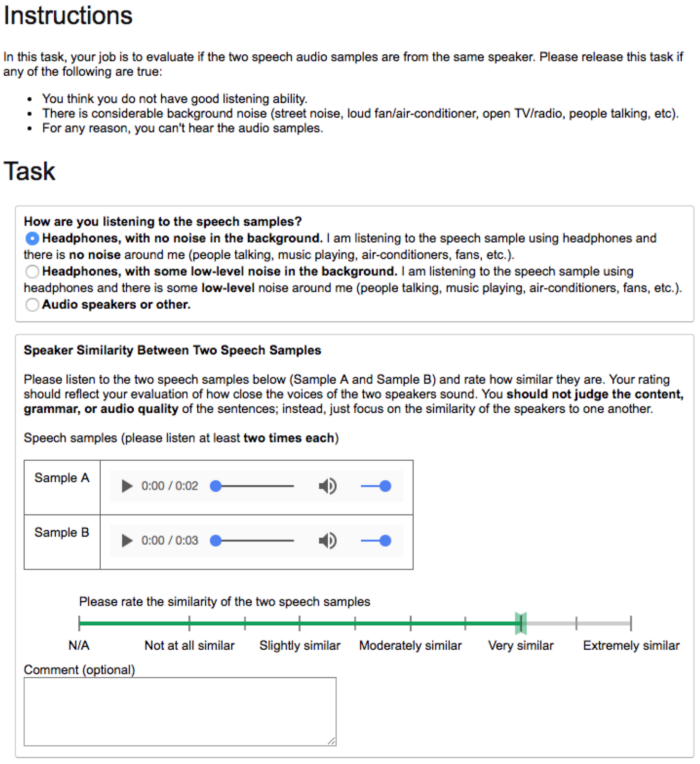
\includegraphics[scale=.45]{figures/nilai}}
        \caption{Pengukuran Kualitas Model\cite{DBLP:journals/corr/abs-1806-04558}}
		\label{nilai}
\end{figure}
Teknik penggunaan rating crowdsourced seperti ini sering disebut dengan Mean Opinion Score atau MOS.
Penulis menemukan bahwa hasil akhir untuk kealamian akhirnya terlihat seperti:
\begin{figure}[H]
        \centerline{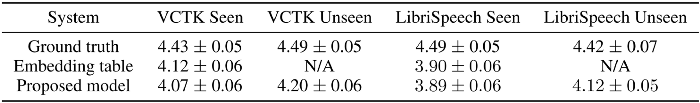
\includegraphics[scale=.45]{figures/hasil}}
        \caption{MOS \cite{DBLP:journals/corr/abs-1806-04558}}
		\label{mos}
\end{figure}

Jika Anda ingin analisis lengkap ini, saya akan merekomendasikan membaca bagian 3.1 dari makalah asli. Namun, secara ringkas:
\begin{enumerate}
\item Model SV2TTS yang diusulkan mencapai sekitar 4,0 MOS di semua kumpulan data.
\item LibriSpeech (salah satu set data pelatihan) diklasifikasikan sebagai kurang alami, karena tidak ada tanda baca dalam transkrip, sehingga menyulitkan model untuk mempelajari jeda.
\item Sistem tabel penyematan menggunakan tabel pencarian penyematan speaker tetapi sebaliknya memiliki arsitektur yang sama. \item Karena memiliki tabel pencarian, tidak dapat digeneralisasi, dan oleh karena itu tidak dapat dievaluasi pada kumpulan data yang tidak terlihat.
\item Kealamian dari contoh yang tidak terlihat dan yang terlihat sangat mirip, yang sangat mengesankan.
\end{enumerate}
Dan untuk kesamaan ucapan, hasilnya terlihat seperti:
\begin{figure}[H]
        \centerline{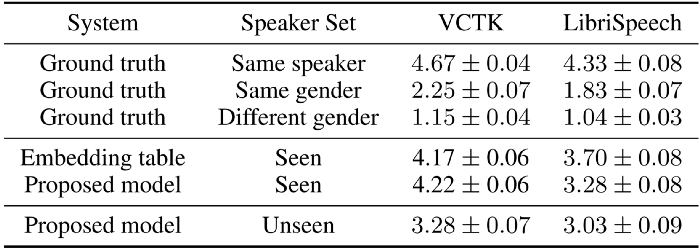
\includegraphics[scale=.35]{figures/hasil1}}
        \caption{Speech Similarity\cite{DBLP:journals/corr/abs-1806-04558}}
		\label{similar}
\end{figure}
Sekali lagi, Anda mungkin ingin membaca bagian 3.2 dari makalah asli untuk analisis lengkapnya. Tapi secara ringkas:
\begin{enumerate}
\item Skor lebih tinggi untuk VCTK (set data pelatihan lainnya), menunjukkan bentuk dataset yang lebih terstruktur.
\item Skor model SV2TTS antara "cukup mirip" dan "sangat mirip" pada skala evaluasi untuk pembicara yang tidak terlihat.
\item Meskipun ini sulit diukur secara matematis, model secara keseluruhan menangkap karakteristik pembicara secara akurat.
\end{enumerate}

\chapter{Multi-Speaker Voice Cloning}
\section{Model SV2TTS}
Model Speech Vector to TTS (SV2TTS) terdiri dari tiga bagian, masing-masing dilatih secara individual.
Hal ini memungkinkan setiap bagian dilatih pada data independen, sehingga mengurangi kebutuhan untuk mendapatkan data multispeaker berkualitas tinggi.

\begin{figure}[H]
        \centerline{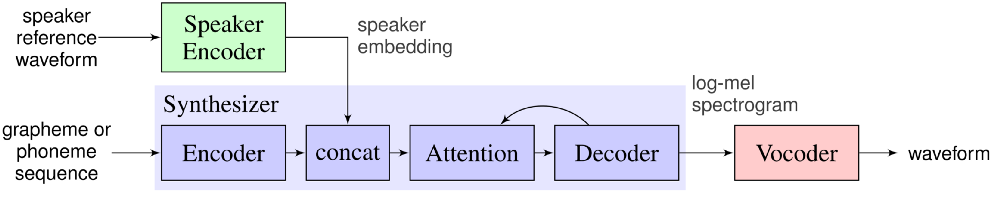
\includegraphics[scale=.35]{figures/arsitektur}}
        \caption{Arsitektur SV2TTS umum Sumber: Jia, Zhang, dan Weiss et al.}
		\label{arsitektur}
\end{figure}

\subsection{Speaker Encoder}

Bagian pertama dari model SV2TTS adalah encoder speaker.
Tugas speaker encoder adalah mengambil beberapa input audio (dikodekan sebagai bingkai spektogram mel), dari speaker tertentu, dan mengeluarkan embedding yang menangkap "bagaimana suara speaker". Encoder pembicara tidak peduli dengan kata-kata yang diucapkan pembicara, atau tentang kebisingan di latar belakang, yang dia pedulikan hanyalah suara pembicara, misalnya, suara bernada tinggi/rendah, aksen, nada, dll. Semua fitur ini digabungkan menjadi vektor berdimensi rendah, yang secara formal dikenal sebagai vektor-d, atau secara informal sebagai penyematan speaker. Akibatnya, ujaran yang diucapkan oleh penutur yang sama akan saling berdekatan pada penyematan penutur, sedangkan tuturan yang diucapkan oleh penutur yang berbeda akan berjauhan pada penyematan penutur\cite{8999436, DBLP:journals/corr/HeigoldMBS15}.
\begin{figure}[H]
        \centerline{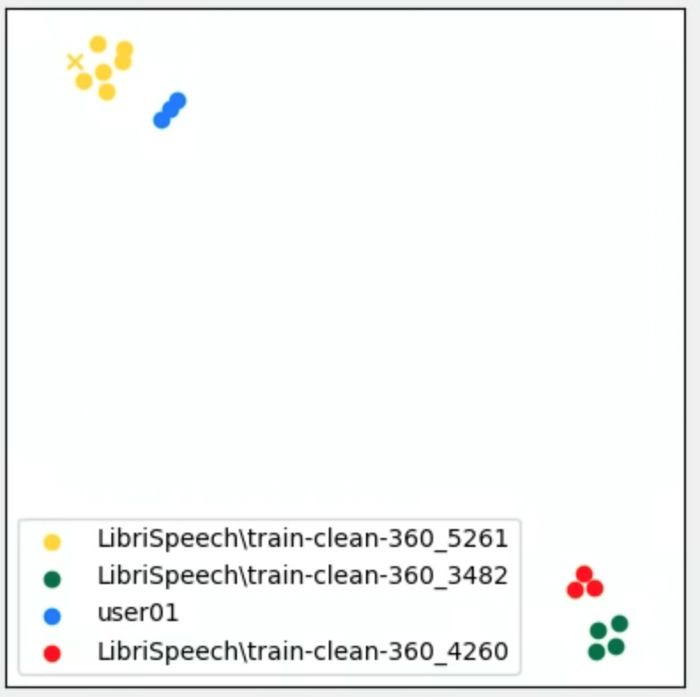
\includegraphics[scale=.35]{figures/encoder}}
        \caption{Representasi visual dari embeddings, setiap warna adalah speaker yang berbeda\cite{DBLP:journals/corr/abs-1806-04558}}
		\label{encoder}
\end{figure}

Untuk belajar menghasilkan embeddings ini, penulis menjelaskan proses berikut:
\begin{enumerate}
\item Pertama, contoh audio ucapan disegmentasi menjadi klip 1,6 detik tanpa transkrip dan diubah menjadi spektogram mel.
\item Kemudian speaker encoder dilatih untuk mengambil dua sampel audio dan memutuskan apakah speaker yang sama memproduksinya atau tidak. Sebagai produk sampingan, ini memaksa encoder speaker untuk membuat embeddings yang mewakili suara speaker.
\end{enumerate}
Proses pelatihan mirip dengan jaringan saraf siam jika Anda sudah familiar dengan mereka.

\subsection{Synthesizer}
Synthesizer adalah bagian dari SV2TTS yang menganalisis input teks untuk membuat spektogram mel, yang kemudian diubah oleh vocoder menjadi suara.
Synthesizer mengambil urutan teks — dipetakan ke fonem (unit terkecil dari suara manusia, misalnya, suara yang Anda buat saat mengucapkan 'a'), bersama dengan embeddings yang dihasilkan oleh encoder speaker, dan menggunakan arsitektur Tacotron 2 untuk menghasilkan bingkai dari spektogram mel secara berulang
\begin{figure}[H]
        \centerline{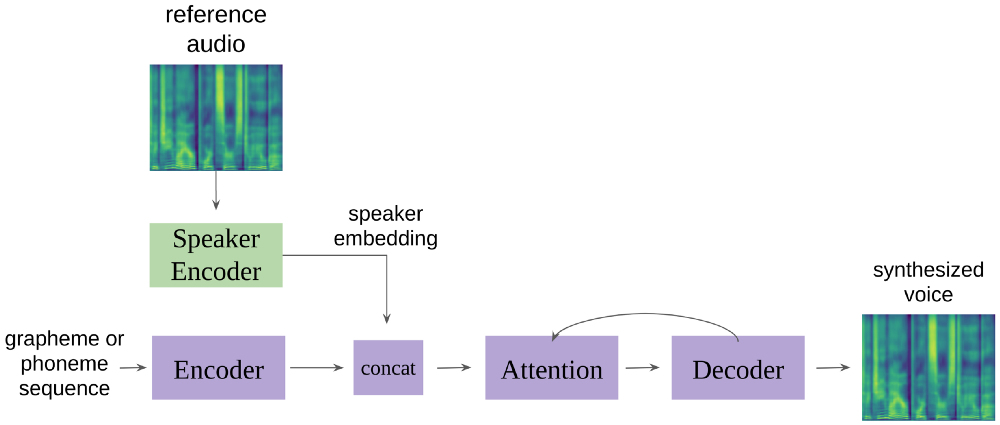
\includegraphics[scale=.35]{figures/model}}
        \caption{Model Arsitektur Multi-Speaker Voice Cloning \cite{DBLP:journals/corr/abs-1806-04558}}
		\label{model}
\end{figure}

Berikut Proses Training Synthesizer:

\begin{enumerate}
\item Pertama, kami mengumpulkan urutan fonem dan spektogram mel dari pembicara yang mengucapkan kalimat itu.
\item Kemudian, spektogram mel diteruskan ke encoder speaker untuk menghasilkan embedding speaker.
\item Selanjutnya, pembuat enkode penyintesis menggabungkan penyandian urutan fonemnya dengan penyematan speaker.
\item Spektogram mel dihasilkan secara berulang oleh decoder dan bagian perhatian dari synthesizer
\item Terakhir, spektogram mel dibandingkan dengan target awal untuk menghasilkan kerugian, yang kemudian dioptimalkan
\end{enumerate}

\begin{figure}[H]
        \centerline{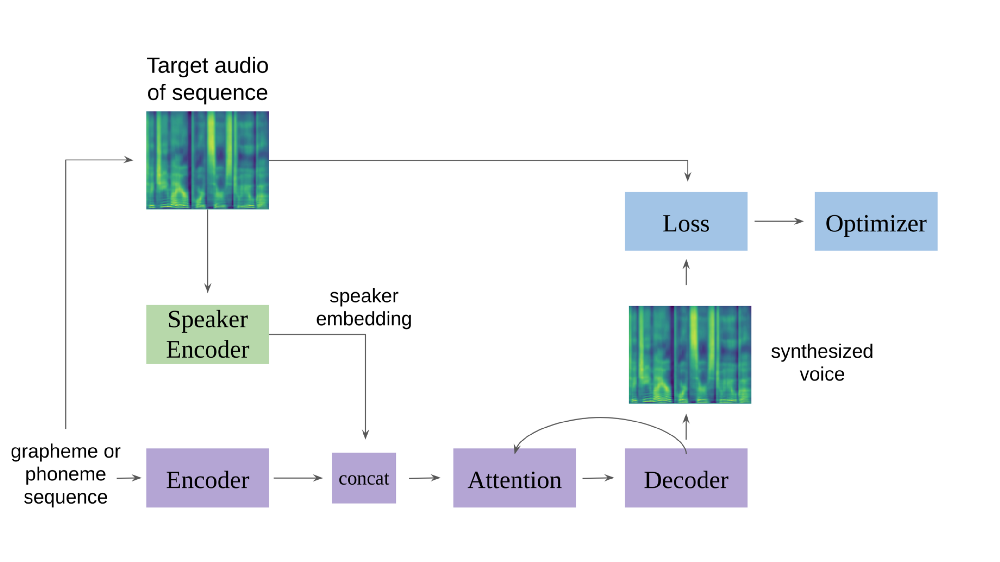
\includegraphics[scale=.35]{figures/train}}
        \caption{Training Synthesizer\cite{DBLP:journals/corr/abs-1806-04558}}
		\label{train}
\end{figure}

\subsection{Vocoder}
Pada titik ini, synthesizer telah membuat spektogram mel, tetapi kami masih belum dapat mendengarkan apa pun. Untuk mengubah spektogram mel menjadi gelombang audio mentah, penulis menggunakan vocoder.
Vocoder khusus yang digunakan di sini didasarkan pada model WaveNet DeepMind , yang menghasilkan bentuk gelombang audio mentah dari teks, dan pada satu titik canggih untuk sistem TTS\cite{DBLP:journals/corr/OordDZSVGKSK16}.
\begin{figure}[H]
        \centerline{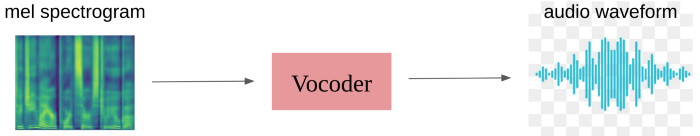
\includegraphics[scale=.35]{figures/vocoder}}
        \caption{Vocoder\cite{DBLP:journals/corr/abs-1806-04558}}
		\label{vocoder}
\end{figure}


\subsection{Alur Model SV2TTS}
berikut adalah alur modelnya:
\begin{enumerate}
\item Encoder speaker mendengarkan sampel audio yang diberikan dan menghasilkan embedding
\item Synthesizer mengambil daftar fonem dan penyematan speaker, kemudian menghasilkan spektogram mel
\item Vocoder saraf menguraikan spektogram mel menjadi bentuk gelombang audio yang dapat kita dengarkan
\end{enumerate}

\subsection{Mengukur Kualitas Hasil}
Penulis menggunakan penilai manusia untuk mengukur kealamian dan kesamaan ucapan yang dihasilkan model.
Kealamian mengukur seberapa "manusia" ucapan itu terdengar, sementara kesamaan mengukur seberapa mirip suara pidato yang disintesis dengan pembicara aslinya.
Penilai berinteraksi melalui GUI yang terlihat seperti:
\begin{figure}[H]
        \centerline{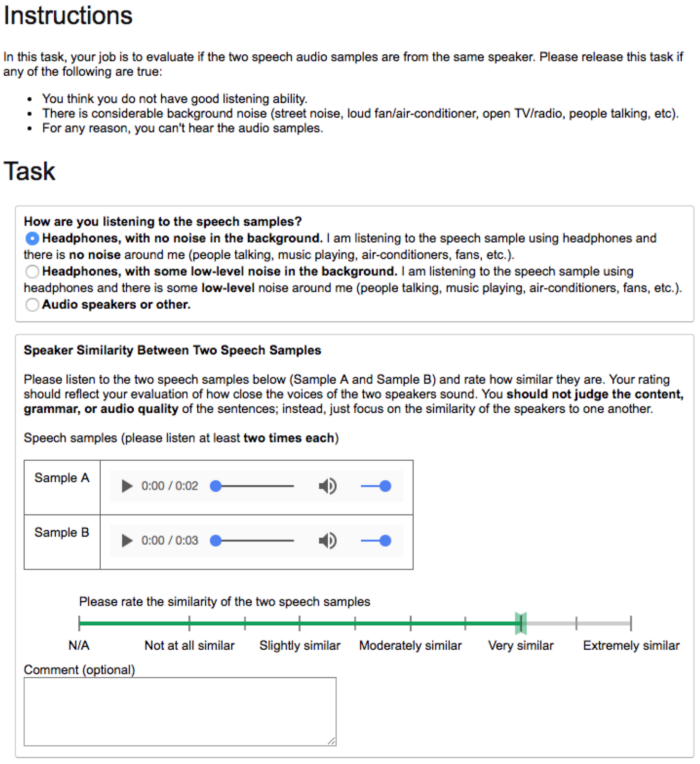
\includegraphics[scale=.45]{figures/nilai}}
        \caption{Pengukuran Kualitas Model\cite{DBLP:journals/corr/abs-1806-04558}}
		\label{nilai}
\end{figure}
Teknik penggunaan rating crowdsourced seperti ini sering disebut dengan Mean Opinion Score atau MOS.
Penulis menemukan bahwa hasil akhir untuk kealamian akhirnya terlihat seperti:
\begin{figure}[H]
        \centerline{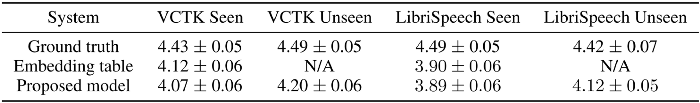
\includegraphics[scale=.45]{figures/hasil}}
        \caption{MOS \cite{DBLP:journals/corr/abs-1806-04558}}
		\label{mos}
\end{figure}

Jika Anda ingin analisis lengkap ini, saya akan merekomendasikan membaca bagian 3.1 dari makalah asli. Namun, secara ringkas:
\begin{enumerate}
\item Model SV2TTS yang diusulkan mencapai sekitar 4,0 MOS di semua kumpulan data.
\item LibriSpeech (salah satu set data pelatihan) diklasifikasikan sebagai kurang alami, karena tidak ada tanda baca dalam transkrip, sehingga menyulitkan model untuk mempelajari jeda.
\item Sistem tabel penyematan menggunakan tabel pencarian penyematan speaker tetapi sebaliknya memiliki arsitektur yang sama. \item Karena memiliki tabel pencarian, tidak dapat digeneralisasi, dan oleh karena itu tidak dapat dievaluasi pada kumpulan data yang tidak terlihat.
\item Kealamian dari contoh yang tidak terlihat dan yang terlihat sangat mirip, yang sangat mengesankan.
\end{enumerate}
Dan untuk kesamaan ucapan, hasilnya terlihat seperti:
\begin{figure}[H]
        \centerline{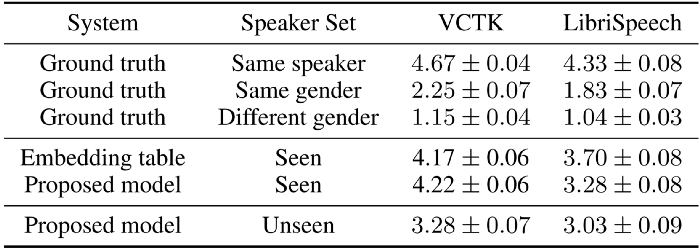
\includegraphics[scale=.35]{figures/hasil1}}
        \caption{Speech Similarity\cite{DBLP:journals/corr/abs-1806-04558}}
		\label{similar}
\end{figure}
Sekali lagi, Anda mungkin ingin membaca bagian 3.2 dari makalah asli untuk analisis lengkapnya. Tapi secara ringkas:
\begin{enumerate}
\item Skor lebih tinggi untuk VCTK (set data pelatihan lainnya), menunjukkan bentuk dataset yang lebih terstruktur.
\item Skor model SV2TTS antara "cukup mirip" dan "sangat mirip" pada skala evaluasi untuk pembicara yang tidak terlihat.
\item Meskipun ini sulit diukur secara matematis, model secara keseluruhan menangkap karakteristik pembicara secara akurat.
\end{enumerate}

\chapter{Tutorial Pembuatan Multi-Speaker Voice Cloning}
\section{Pengenalan Anaconda}
Anaconda merupakan sebuah software yang mendistribusikan bahasa pemrograman python dan R untuk keperluan komputasi ilmiah seperti data science, machine learning, data processing skala-luas, analisis prediksi, dan lain sebaginya.
Anaconda memiliki anaconda navigator yang didalamnya terdapat software-software yang dapat digunakan untuk membuat program python dan R. Salah satu software yang akan kita gunakan yaitu Spyder. Sebelum kita membuat program kita harus menginstal anaconda terlebih dahulu.
Instalasi pada kali ini menggunakan 2 sistem operasi yaitu Windows 10 x64 dan Ubuntu 19.04. Hal yang dibutuhkan adalah laptop dengan os windows atau ubuntu dan internet.
\subsection{Instalasi Anaconda 3 Windows 10 x64}
Hal yang harus diperhatikan sebelum melakukan instalasi \textit{Anaconda Python}
\begin{enumerate}
 \item \textit{Download Anaconda Python} https://www.anaconda.com/distribution/
 \item Perhatikan versi dari sistem operasi yang digunakan (versi 32bit atau 64bit)
 \item Download file anaconda yang sesuai dengan versi sistem operasi (32bit atau 64bit)
\end{enumerate}

Berikut langkah-langkah instalasi anaconda.
\begin{enumerate}
\item Buka aplikasi \textit{installer Anaconda} yang telah didwonload lalu akan muncul  gambar \ref{langkah1}, lalu pilih run untuk menjalankan proses instalasi. 
\begin{figure}[H]
        \centerline{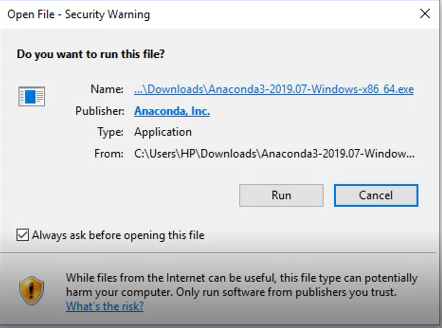
\includegraphics[scale=0.75]{figures/1}}
        \caption{Run Setup Anaconda}
		\label{langkah1}
\end{figure}

\item Tunggu hingga \textit{setup loading} selesai seperti pada gambar \ref{langkah2}.
\begin{figure}[H]
        \centerline{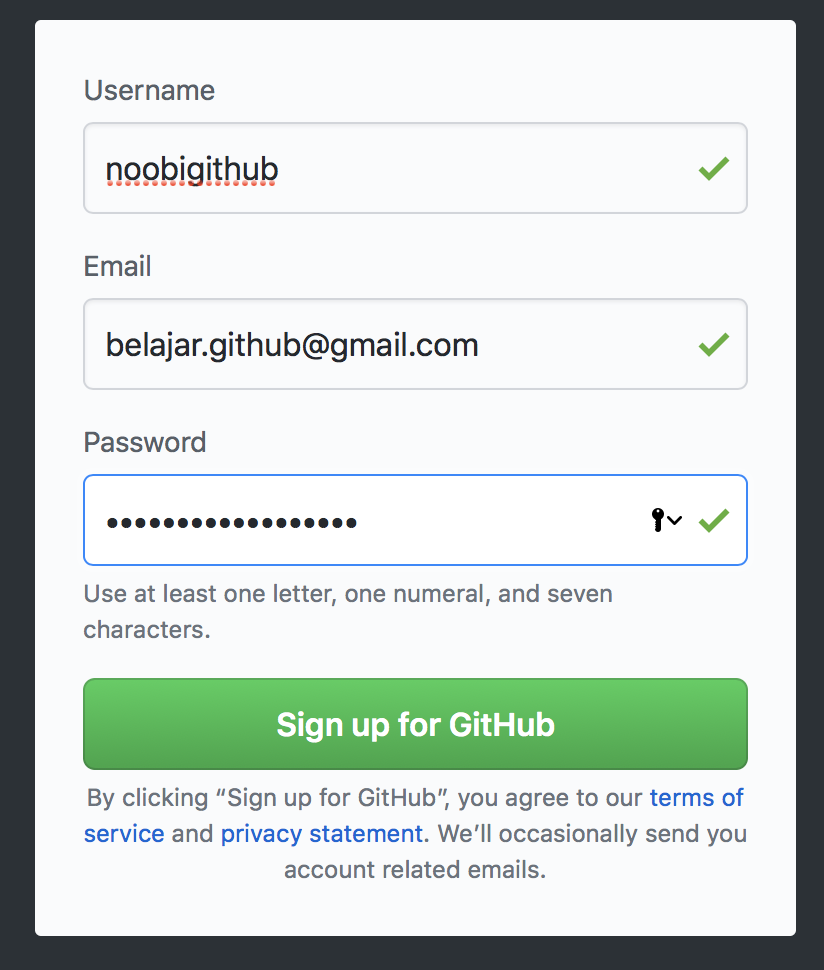
\includegraphics[scale=0.75]{figures/2}}
        \caption{Setup Loading}
		\label{langkah2}
\end{figure}

\item Jika \textit{setup loading} telah selesai, maka klik \textit{next} seperti pada gambar \ref{langkah3}.
\begin{figure}[H]
        \centerline{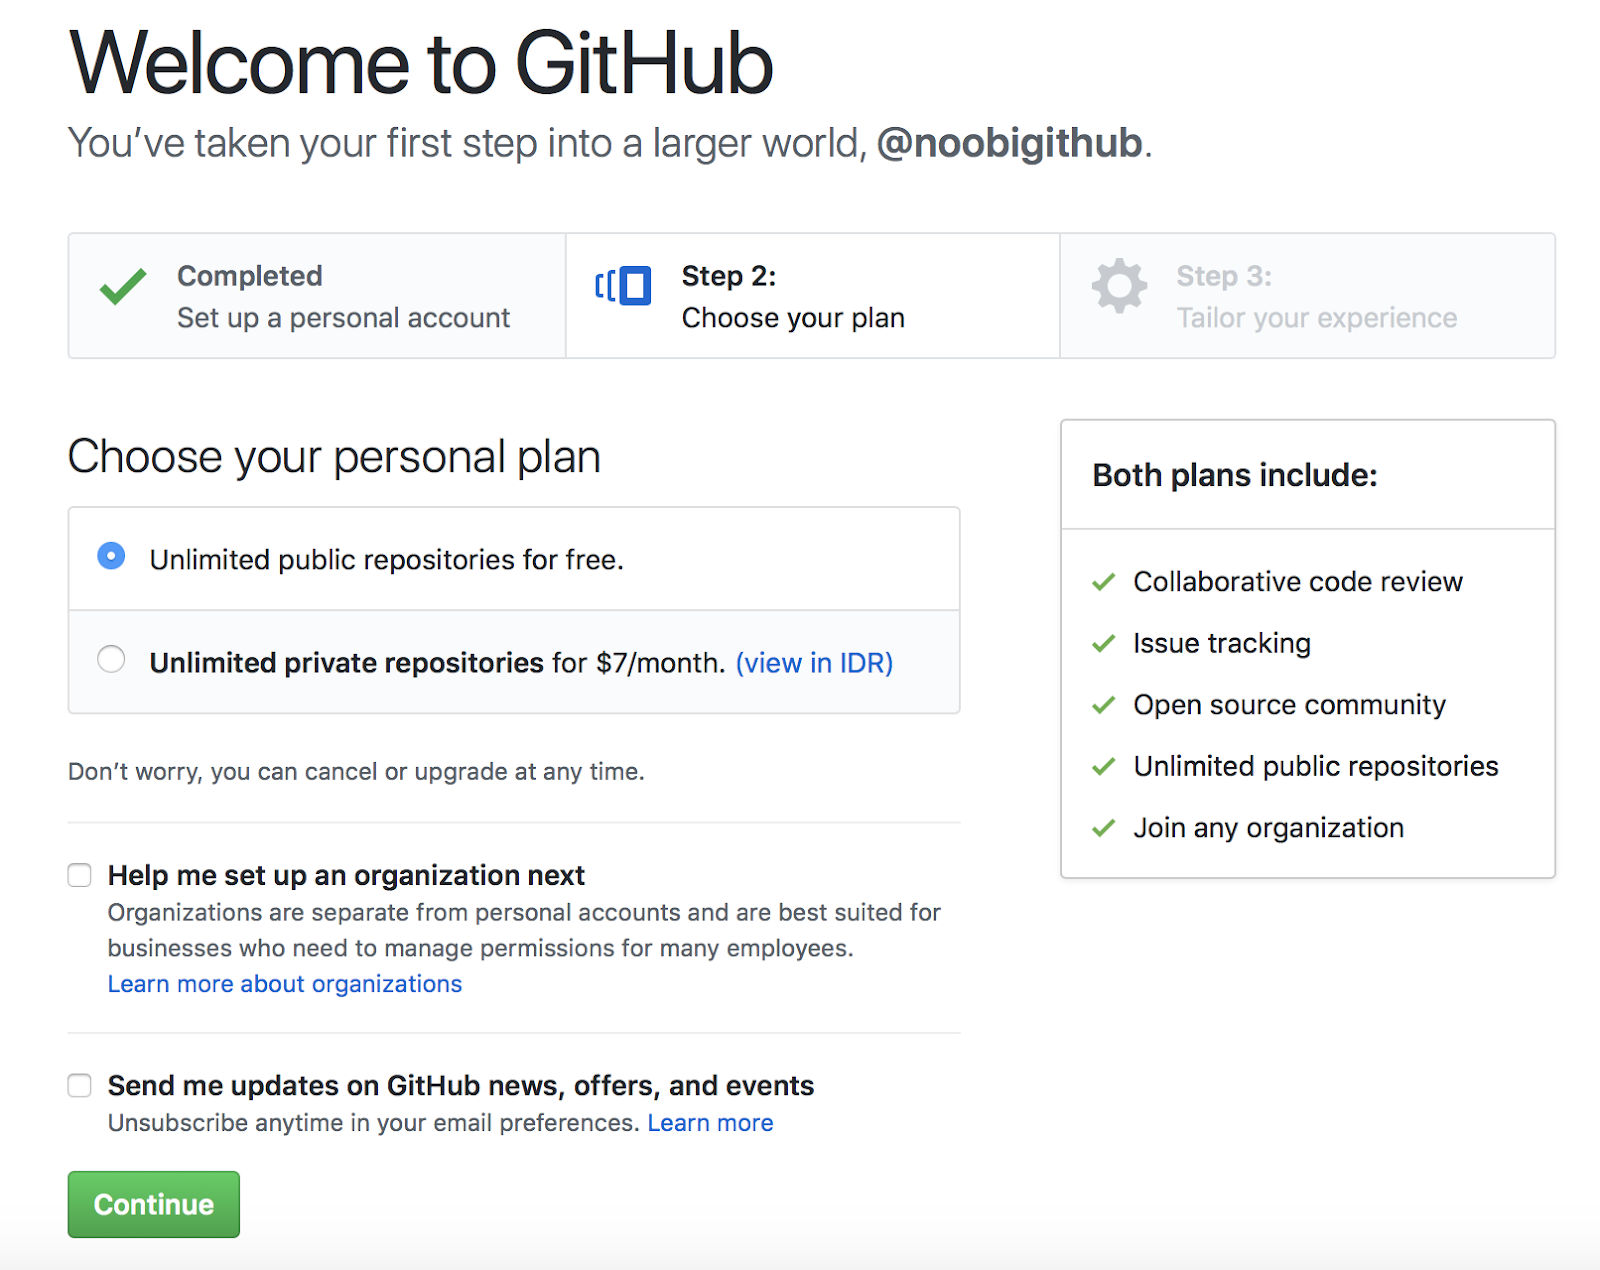
\includegraphics[scale=0.75]{figures/3}}
        \caption{Welcome to Anaconda Setup}
		\label{langkah3}
\end{figure}

\item Pada \textit{License Agreement} klik \textit{I Agree} karena jika teman-teman tidak menyetujui lisensi anaconda maka teman-teman tidak akan bisa melanjutkan proses instalasi. lakukan langkah ini seperti pada gambar \ref{Figureanaconda3}

\begin{figure}[H]
    \centering
    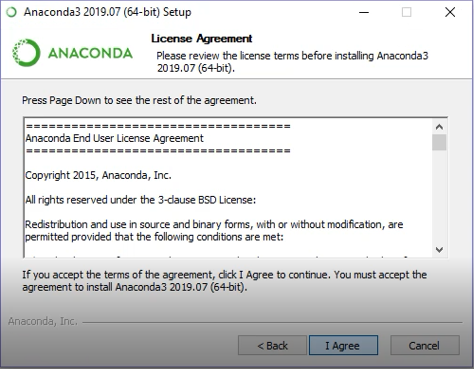
\includegraphics[scale=0.75]{figures/4}
    \caption{\textit{License Agreement}}
    \label{Figureanaconda3}
\end{figure}


\item Kemudian pilih \textit{Just Me(Recomended)} agar sesuai dengan komputer yang digunakan, kemudian klik \textit{next} seperti pada gambar \ref{Figureanaconda4}.

\begin{figure}[H]
    \centerline{\includegraphics[scale=0.75]{figures/5}}
    \caption{\textit{Just Me(recomended)}}
    \label{Figureanaconda4}
\end{figure}


\item Kemudian pilih directori tempat kita akan \textit{menginstall anaconda} seperti pada gambar \ref{Figureanaconda5}

\begin{figure}[H]
    \centering
    \includegraphics[scale=0.75]{figures/6}
    \caption{\textit{Pilih lokasi}}
    \label{Figureanaconda5}
\end{figure}

\item Kemudian centang \textit{Add Anaconda to my Path environtment variable}, agar saat melakukan instalasi  \textit{package anaconda, package} tersebut akan langsung tertuju ke \textit{path anaconda} tidak ke aplikasi yang lain. kemudian Klik \textit{install} seperti pada gambar \ref{Figureanaconda6}.

\begin{figure}[H]
    \centering
    \includegraphics[scale=0.75]{figures/7}
    \caption{\textit{Centang Anaconda to my PATH}}
    \label{Figureanaconda6}
\end{figure}

\item Tunggu sampai proses \textit{installasi} selesai seperti pada gambar \ref{Figureanaconda7}.

\begin{figure}[H]
    \centering
    \includegraphics[scale=0.75]{figures/8}
    \caption{\textit{Waiting Installation Complete}}
    \label{Figureanaconda7}
\end{figure}

\item Apabila instalasi telah selesai  maka akan terlihat seperti gambar \ref{Figureanaconda8}, kemudian klik \textit{next}
\begin{figure}[H]
    \centering
    \includegraphics[scale=0.75]{figures/9}
    \caption{\textit{Installation Complete}}
    \label{Figureanaconda8}
\end{figure}

\item apabila muncul gambar \ref{Figureanaconda70}, maka klik \textit{next}
\begin{figure}[H]
    \centering
    \includegraphics[scale=0.75]{figures/10}
    \caption{\textit{Anaconda+JetBrains}}
    \label{Figureanaconda70}
\end{figure}

\item Jika instalasi telah selesai maka akan ada ucapan terima kasih telah menginstall anaconda 3 seperti pada gambar \ref{Figureanaconda9}, hal ini menandakan bahwa teman-teman telah selesai dan berhasil melakukan instalasi anaconda. Kemudian klik \textit{finish} untuk mengakhiri instalasi.

\begin{figure}[H]
    \centering
    \includegraphics[scale=0.75]{figures/11}
    \caption{\textit{Thanks for install Anaconda}}
    \label{Figureanaconda9}
\end{figure}
\end{enumerate}

\subsection{Update Anaconda dan Spyder}
Kenapa kita harus melakukan update anaconda dan spyder? melakukan update diperlukan agar software yang kita gunakan merupakan software yang terbaru, karena versi lama dan versi baru akan memiliki banyak perbedaan dan akan menjadi masalah nantinya ketika kita membuat program atau mengimportkan modul-modul python yang digunakan.
Berikut cara mengupdate Spyder:
\begin{enumerate}
\item Buka anaconda prompt, lalu ketikkan perintah conda update spyder
\item Konfirmasi update dengan mengetikkan y, lalu tekan enter
\item Tunggu hingga installan selesai
\end{enumerate}
Berikut cara mengupdate Anaconda:
\begin{enumerate}
\item Buka anaconda prompt, lalu ketikkan perintah conda update anaconda
\item Konfirmasi update anaconda dengan mengetikkan y dan kemudian tekan enter
\item Tunggu hingga installan selesai
\end{enumerate}

\subsection{Instalasi Anaconda Ubuntu 19.04}
Untuk instalasi python pada Ubuntu 19.04 dibutuhkan sebagai berikut:

\begin{enumerate}
\item Internet
\item Anaconda installer (64bit or 32bit)
\item enter, dan yes atau no
\end{enumerate}

Ikuti langkah berikut:
\begin{enumerate}
\item Pertama kita kunjungi situs \textbf{\textit{https://www.anaconda.com/distribution/\#download-section}} seperti gambar ~\ref{anacondadownload} dan pilih \textbf{64-Bit (x86) Installer (517 MB)}
\begin{figure}[H]
\centering
\includegraphics[width=1\textwidth]{figures/ubuntu/anacondadownload.png}
\caption{Gambar halaman download}
\label{anacondadownload}
\end{figure}

\item Kedua kita buka \textit{\textbf{terminal}} kita lalu arahkan ke direktori kita menyimpan file download anaconda

\item Ketiga kita ketikkan sebagai berikut \textbf{bash \textit{namafileanaconda}.sh} lalu enter, contoh seberti gambar \ref{anacondabash}
\begin{figure}[H]
\centering
\includegraphics[width=1\textwidth]{figures/ubuntu/anacondabash.png}
\caption{Gambar install anaconda}
\label{anacondabash}
\end{figure}

\item Setelah itu, tekan \textbf{ENTER} saja seperti gambar \ref{anacondaenter}
\begin{figure}[H]
\centering
\includegraphics[width=1\textwidth]{figures/ubuntu/anacondaenter.png}
\caption{Gambar eksekusi anaconda}
\label{anacondaenter}
\end{figure}

\item Lalu akan muncul sebuah tulisan \textbf{End User License Agreement} seperti gambar \ref{entertrus}, tekan \textbf{ENTER} dan tahan hingga seperti gambar 
\begin{figure}[H]
\centering
\includegraphics[width=1\textwidth]{figures/ubuntu/entertrus.png}
\caption{Gambar anaconda license agreement}
\label{entertrus}
\end{figure}
\begin{figure}[H]
\centering
\includegraphics[width=1\textwidth]{figures/ubuntu/enterkekgini.png}
\caption{Gambar perintah yes or no}
\label{enterkekgini}
\end{figure}

\item Lalu setelah muncur perintah \textbf{\textit{'yes' or 'no'}} ketik \textbf{\textit{yes}} lalu enter

\item Setelah itu muncul path direktori instalasi anaconda kita seperti gambar \ref{enterpath} lalu tekan enter
\begin{figure}[H]
\centering
\includegraphics[width=1\textwidth]{figures/ubuntu/enterpath.png}
\caption{Gambar path anaconda}
\label{enterpath}
\end{figure}

Setelah kita selesai instalasi anaconda jangan lupa juga untuk menginstal spyder ide, caranya seperti berikut:
\begin{enumerate}

\item ketikkan perintah \textbf{\textit{sudo apt install spyder3 -y}} seperti gambar \ref{installspyder3}
\begin{figure}[H]
\centering
\includegraphics[width=1\textwidth]{figures/ubuntu/installspyder3.png}
\caption{Gambar perintah install spyder3}
\label{installspyder3}
\end{figure}

\item lalu jalankan dengan perintah \textbf{\textit{spyder}} atau \textbf{\textit{spyder3}}
\end{enumerate}

\end{enumerate}

\subsection{Konfigurasi \textbf{\textit{Python}}}
Setelah kita selesai instal Anaconda dan Spyder, selanjutnya kita akan mempelajari bagaimana cara setting environments python kita? caranya sebagai berikut

\begin{enumerate}

\item pertama kita buka terminal kita lalu ketikkan perintah \textbf{export PYTHONPATH=\$PYTHONPATH:\textit{pathinstallasipythonkalian}} contoh seperti gambar \ref{setpath}, lalu enter
\begin{figure}[H]
\centering
\includegraphics[width=1\textwidth]{figures/ubuntu/setpath.png}
\caption{Gambar setpath}
\label{setpath}
\end{figure}

\end{enumerate}

\section{Instalasi Pycharm}
Ikuti langkah-langkah berikut untuk install pycharm di sistem operasi windows:
\begin{enumerate}
\item Download Installer Pycharm dari situs resminya yaitu  https://www.jetbrains.com/pycharm/download.
\item Jalankan Installer PyCharm yang telah selesai di download, kemudian klik Next untuk melanjutkan installasi seperti pada contoh gambar \ref{installpycharm}.
\begin{figure}[H]
\centering
\includegraphics[scale=.65]{figures/install_pycharm1}
\caption{Klik Next untuk Install Pycharm}
\label{installpycharm}
\end{figure}
\item Tentukan destination folder jika diperlukan, atau dibiarkan default kemudian klik Next.
\begin{figure}[H]
\centering
\includegraphics[scale=.65]{figures/install_pycharm2}
\caption{Menentukan lokasi folder dan klik next}
\label{installpycharm1}
\end{figure}
\item Checklist pada "Add launchers dir to PATH" kemudian klik Next.
\begin{figure}[H]
\centering
\includegraphics[scale=.65]{figures/install_pycharm3}
\caption{Add launchers dir to PATH}
\label{installpycharm3}
\end{figure}
\item Klik Install untuk melanjutkan
\begin{figure}[H]
\centering
\includegraphics[scale=.65]{figures/install_pycharm4}
\caption{Klik Install}
\label{installpycharm4}
\end{figure}
\item Tunggu proses installasi PyCharm sampai selesai.
\begin{figure}[H]
\centering
\includegraphics[scale=.65]{figures/install_pycharm6}
\caption{Reboot Now}
\label{installpycharm6}
\end{figure}
\item Setelah proses installasi PyCharm selesai, klik Reboot now, lalu klik Finish.
\end{enumerate}

\section{Membuat Akun Github}
Github merupakan software developer untuk menyimpan dan sharing project-project yang bersifat opensource, karena bersifat opensource maka project tersebut dapat dikembangkan oleh programmer lain yang ingin berkontribusi pada project, sangat bagus untuk project yang dikembangkan oleh team maupun individu. 

Github memiliki banyak keunggulan diantaranya sebagai tempat menyimpan backup project, adanya free hosting, memudahkan developer, mendukung semua bahasa pemrograman dan github juga berguna sebagai tempat penyimpanan project secara gratis.

Berikut tata cara membuat akun github:
\begin{enumerate}
\item buka browser kemudian kunjungi situs github.
\item kliktombol sign up
\begin{figure}[H]
\centering
\includegraphics[scale=.25]{figures/daftar}
\caption{Sign Up | sumber: https://omcyber.com/cara-membuat-akun-github/}
\label{git2}
\end{figure}
\item isi formulir data diri seperti username, email, password, dan verify your account. Pastikan data yang diisikan benar.
\begin{figure}[H]
\centering
\includegraphics[scale=.25]{figures/form}
\caption{Form Daftar}
\label{git3}
\end{figure}
\item klik tombol create an account untuk membuat akun baru github.
\item silahkan pilih free plan dengan klik tombol jon a free plan
\begin{figure}[H]
\centering
\includegraphics[scale=.25]{figures/free}
\caption{Free Plan}
\label{git4}
\end{figure}
\item verifikasi email agar akun github terverifikasi
\begin{figure}[H]
\centering
\includegraphics[scale=.25]{figures/verifikasi}
\caption{Verifikasi Email}
\label{git5}
\end{figure}
\item buka inbox email yang didaftarkan, buka email dari github dan klik verifikasi email address.
\begin{figure}[H]
\centering
\includegraphics[scale=.25]{figures/email}
\caption{Verifikasi Email Address}
\label{git5}
\end{figure}
\item setelah berhasil verifikasi email maka akun github telah berhasil dibuat dan terverifikasi.
\begin{figure}[H]
\centering
\includegraphics[scale=.25]{figures/berhasil}
\caption{Verifikasi Email Berhasil}
\label{git6}
\end{figure}
\end{enumerate}

\section{Download dan Install Git}
Sebelum melakukan instalasi git, kita memerlukan file instalasi git terlebih dahulu. File ini bisa teman-teman dapatkan dengan mengunduh file dari situs resmi git, berikut link yang dapat teman-teman kunjungi https://git-scm.com/downloads. Download file yang sesuai dengan sistem operasi pada komputer teman-teman. Jika komputer teman-teman memiliki sistem operasi Windows 64bit maka teman-teman harus mengunduh file instalasi git untuk windows 64bit. Ikuti tahapan berikut untuk melakukan instalasi git:
\begin{enumerate}
\item Buka file instalasi git yang telah di download, kemudian klik next.
\begin{figure}[H]
\centering
\includegraphics[scale=.5]{figures/install_git1}
\caption{Install Git}
\label{install_git1}
\end{figure}

\item Pilih lokasi instalasi git, disarankan install pada lokasi seperti gambar
\begin{figure}[H]
\centering
\includegraphics[scale=.5]{figures/install_git2}
\caption{Lokasi Instalasi Git}
\label{install_git2}
\end{figure}

\item Selanjutnya pilih komponen tambahan untuk install git, sesuaikan dengan kebutuhan teman-teman. Jika sudah maka klik next untuk melanjutkan instalasi.
\begin{figure}[H]
\centering
\includegraphics[scale=.5]{figures/install_git3}
\caption{Komponen Tambahan}
\label{install_git3}
\end{figure}

\item Tentukan nama aplikasi git, untuk memudahkan pencarian aplikasi maka disarankan menggunakan nama Git saja.
\begin{figure}[H]
\centering
\includegraphics[scale=.35]{figures/install_git4}
\caption{Select Start Menu Folder}
\label{install_git4}
\end{figure}

\item pilih file editor untuk dikombinasikan dengan git, pada tutorial ini saya menggunakan vim editor lalu pilih next.
\begin{figure}[H]
\centering
\includegraphics[scale=.5]{figures/install_git5}
\caption{Choose Default Editor}
\label{install_git5}
\end{figure}

\item selanjutnya kita perlu mengatur path environment, Pilih Git from the command line and also from 3rd-party software agar saat menjalankan perintah Git dapat dikenali di Command Prompt (CMD) pada Windows.
\begin{figure}[H]
\centering
\includegraphics[scale=.5]{figures/install_git6}
\caption{PATH Environment}
\label{install_git6}
\end{figure}

\item kemudian pilih aplikasi SSH, pada tutorial ini saya memilih Use OpenSSH yang merupakan aplikasi default SSH dari Git lalu klik next.
\begin{figure}[H]
\centering
\includegraphics[scale=.5]{figures/install_git7}
\caption{Choose SSH}
\label{install_git7}
\end{figure}

\item selanjutnya pilih Checkout Windows-style, commit Unix-style line endings dan klik next
\begin{figure}[H]
\centering
\includegraphics[scale=.5]{figures/install_git8}
\caption{Configuring the line ending}
\label{install_git8}
\end{figure}

\item pilih Use Windows’ default console windows kemudian klik next
\begin{figure}[H]
\centering
\includegraphics[scale=.5]{figures/install_git9}
\caption{Configuring the terminal emulator}
\label{install_git9}
\end{figure}

\item pilih opsi ekstra yaitu Enable File System Caching agar Git memiliki fungsi system caching dan Enable Git Credential Manager agar Git bisa dikombinasikan dengan aplikasi lain seperti Visual Studio, Android Studio, dan GitHub. Selanjutnya klik next.
\begin{figure}[H]
\centering
\includegraphics[scale=.5]{figures/install_git10}
\caption{Configuring extra options}
\label{install_git10}
\end{figure}

\item setelah menambahkan konfigurasi ekstra maka teman-teman bisa melakukan instalasi git dengan klik install.
\begin{figure}[H]
\centering
\includegraphics[scale=.5]{figures/install_git11}
\caption{Install}
\label{install_git11}
\end{figure}

\item Tunggu hingga proses instalasi selesai.
\begin{figure}[H]
\centering
\includegraphics[scale=.5]{figures/install_git12}
\caption{Proses Install}
\label{install_git12}
\end{figure}

\item Jika instalasi telah selesai maka teman-teman bisa cek versi git untuk memastikan apakah git telah berhasil terinstal di komputer teman-teman dengan membuka command prompt atau cmd.
\begin{figure}[H]
\centering
\includegraphics[scale=.5]{figures/install_git13}
\caption{Command Prompt (CMD)}
\label{install_git13}
\end{figure}

\item ketikkan perintah git --version lalu tekan enter untuk melihat versi git yang telah teman-teman install.
\begin{figure}[H]
\centering
\includegraphics[scale=.35]{figures/install_git14}
\caption{Versi Git}
\label{install_git14}
\end{figure}

\end{enumerate}

\section{Konfigurasi Git}
Berikut hal yang perlu teman-teman lakukan apabila telah install git di komputer, teman-teman perlu melakukan konfigurasi email dan username akun git teman-teman. Ikuti tahapan berikut untuk melakukan konfigurasi git:
\begin{enumerate}
\item Konfigurasikan email dan username git yang telah teman-teman daftarkan pada github dengan mengetikkan perintah
\begin{verbatim}
git config --global user.name "username anda"
git config --global user.email "email_anda@gmail.com"
\end{verbatim}
\begin{figure}[H]
\centering
\includegraphics[scale=.75]{figures/konfig_git1}
\caption{Konfigurasi Username Git}
\label{konfig_git1}
\end{figure}

\begin{figure}[H]
\centering
\includegraphics[scale=.75]{figures/konfig_git2}
\caption{Konfigurasi Email Git}
\label{konfig_git2}
\end{figure}

\item membuat ssh key dengan mengetikkan perintah
\begin{verbatim}
ssh-keygen -t rsa -b 4096 -C "email_anda@gmail.com"
\end{verbatim}
lalu tekan enter sebanyak tiga kali, pertama untuk membuat direktori penyimpanan ssh, kedua dan ketiga untuk menambahkan passphrase.
\begin{figure}[H]
\centering
\includegraphics[scale=.75]{figures/konfig_git3}
\caption{Generate SSH key}
\label{konfig_git3}
\end{figure}

\item jika ssh key telah berhasil digenerate, ketikkan perintah
\begin{verbatim}
cd .ssh/
ls
\end{verbatim}
perintah ini digunakan untuk berpindah direktori ke direktori ssh dan menampilkan list file yang ada didalam direktori tersebut.
\begin{figure}[H]
\centering
\includegraphics[scale=.5]{figures/konfig_git4}
\caption{Direktori SSH}
\label{konfig_git4}
\end{figure}

\item ketikkan perintah berikut untuk menampilkan ssh yang telah digenerate, kemudian copy ssh key yang tampil dilayar teman-teman.
\begin{verbatim}
cat id_rsa.pub
\end{verbatim}

\begin{figure}[H]
\centering
\includegraphics[scale=.5]{figures/konfig_git5}
\caption{SSH Key}
\label{konfig_git5}
\end{figure}

\item pilih menu SSH dan GPG keys
\begin{figure}[H]
\centering
\includegraphics[scale=.35]{figures/konfig_git7}
\caption{Menu  SSH dan GPG keys}
\label{konfig_git7}
\end{figure}

\item klik tombol New SSH key
\begin{figure}[H]
\centering
\includegraphics[scale=.35]{figures/konfig_git8}
\caption{New SSH key}
\label{konfig_git8}
\end{figure}

\item isikan title, pada bagian key paste ssh key yang telah di copy sebelumnya dan klik add SSH key
\begin{figure}[H]
\centering
\includegraphics[scale=.5]{figures/konfig_git9}
\caption{Add SSH key}
\label{konfig_git9}
\end{figure}

\item sekarang teman-teman telah berhasil menambahkan ssh key pada akun github teman-teman. Selanjutnya teman-teman dapat mengklon Real-Time-Voice-Cloning project.

\end{enumerate}

\section{Fork dan Clone Voice Cloning Repositori}
berikut tutorial clone repo voice cloning menggunakan github:
\begin{enumerate}
\item Kunjungi link berikut https://github.com/dindamajesty13/Real-Time-Voice-Cloning
\item Klik fork, maka repo Real-Time-Voice-Cloning akan ada di github anda.
\begin{figure}[H]
\centering
\includegraphics[scale=.3]{figures/repo}
\caption{Fork Repositori}
\label{repo1}
\end{figure}

\item buka project Real-Time-Voice-Cloning yang ada direpo anda lalu klik pada bagian code.
\begin{figure}[H]
\centering
\includegraphics[scale=.3]{figures/repo1}
\caption{Klik Tombol Code}
\label{repo2}
\end{figure}

\item pilih HTTPS dan salin url yang ada dibawah tulisan HTTPS
\begin{figure}[H]
\centering
\includegraphics[scale=.75]{figures/repo3}
\caption{Copy Url}
\label{repo3}
\end{figure}

\item buka gitbash kemudian ketikkan git clone lalu paste url yang telah di copy sebelumnya.
\begin{figure}[H]
\centering
\includegraphics[scale=.4]{figures/repo4}
\caption{Git Clone Repositori}
\label{repo4}
\end{figure}

\item Lalu tekan enter pada keyboard, tunggu hingga proses clone selesai.
\begin{figure}[H]
\centering
\includegraphics[scale=.4]{figures/repo5}
\caption{Proses Clone Repositori}
\label{repo5}
\end{figure}

\item jika proses clone telah selesai, buka pycharm.

\item klik menu file, pilih open.
\begin{figure}[H]
\centering
\includegraphics[scale=.2]{figures/repo6}
\caption{Pycharm}
\label{repo6}
\end{figure}

\item cari folder Real-Time-Voice-Cloning, kemudian klik ok
\begin{figure}[H]
\centering
\includegraphics[scale=.55]{figures/repo7}
\caption{Lokasi Folder Repositori}
\label{repo7}
\end{figure}

\item pycharm akan membuka file project Real-Time-Voice-Cloning, jika terdapat pop up create virtual environment klik ok jika versi python sama dengan 3.7, jika versi python 3.9 seperti gambar \ref{repo8} maka klik cancel dan ikuti tahapan Menambahkan Interpreter ke dalam Voice Cloning Project dibawah.
\begin{figure}[H]
\centering
\includegraphics[scale=.55]{figures/repo8}
\caption{Pop Up Create Virtual Environment}
\label{repo8}
\end{figure}

\item jika berhasil maka anda akan melihat tampilan seperti pada gambar \ref{repo9}
\begin{figure}[H]
\centering
\includegraphics[scale=.3]{figures/repo9}
\caption{Real-Time-Voice-Cloning project}
\label{repo9}
\end{figure}

\end{enumerate}

\section{Menambahkan Interpreter ke dalam Voice Cloning Project} 
Sebelum menjalankan project menggunakan Pycharm kita membutuhkan interpreter, saya menyarankan untuk menggunakan virtual environment atau conda environment jika anda pengguna anaconda. Dalam pembuatan interpreter penggunaan python 3.7 sangat direkomendasikan karena pada pembuatan voice cloning ini menggunakan tensorflow versi 1.x sehingga teman-teman harus mendownload python versi 3.7, ffmpeg, pytorch, dan requirements.
Berikut tata pembuatan virtual environment untuk project voice cloning ini:

\subsection{Download dan Install Python 3.7}
\begin{enumerate}
\item download python versi 3.7 pada website resmi python atau kunjungi link berikut https://www.python.org/downloads/release/python-371/

\item Pilih file yang sesuai dengan sistem operasi dan processor pada komputer teman-teman.
\begin{figure}[H]
\centering
\includegraphics[scale=.4]{figures/python1}
\caption{Download Python 3.7}
\label{python1}
\end{figure}

\item Centang add python 3.7 to PATH agar python yang diinstal ditambahkan ke environment variabel komputer teman-teman, kemudian klik install now.
\begin{figure}[H]
\centering
\includegraphics[scale=.4]{figures/python2}
\caption{Add Python to PATH}
\label{python2}
\end{figure}

\item Jika instalasi telah selesai maka teman-teman akan melihat tampilan seperti gambar \ref{python3}
\begin{figure}[H]
\centering
\includegraphics[scale=.4]{figures/python3}
\caption{Success Install Python 3.7}
\label{python3}
\end{figure}

\item Untuk memastikan apakah python 3.7 telah benar-benar berhasil terinstal teman-teman dapat melakukan pengecekan melalui command prompt (CMD) dengan mengetikkan perintah python kemudian tekan enter.
\begin{figure}[H]
\centering
\includegraphics[scale=.4]{figures/python4}
\caption{Check Python Version}
\label{python4}
\end{figure}

\end{enumerate}

\subsection{Download dan Install FFmpeg}

\begin{enumerate}

\item Setelah menginstal python 3.7, kita harus menginstal ffmpeg, kunjungi link berikut untuk mendapatkan file instalasi ffmpeg https://ffmpeg.org/download.html. Sesuaikan file download dengan sistem operasi yang teman-teman gunakan. Pada tutorial ini saya menggunalan system operasi windows.
\begin{figure}[H]
\centering
\includegraphics[scale=.35]{figures/python5}
\caption{Download FFmpeg}
\label{python5}
\end{figure}

\item Pilih Windows builds from gyan.dev. Kemudian teman-teman akan diarahkan ke halaman seperti pada gambar \ref{python6}
\begin{figure}[H]
\centering
\includegraphics[scale=.4]{figures/python6}
\caption{Download FFmpeg for Windows}
\label{python6}
\end{figure}

\item Download file ffmpeg-git-full.7z kemudian extract file instalasi FFmpeg yang telah didownload.
\begin{figure}[H]
\centering
\includegraphics[scale=1.5]{figures/python7}
\caption{Extract File Instalasi}
\label{python7}
\end{figure}

\item Ganti nama direktori menjadi FFmpeg
\begin{figure}[H]
\centering
\includegraphics[scale=1.5]{figures/python8}
\caption{Ganti Nama Folder}
\label{python8}
\end{figure}

\item Copy folder dan Paste folder ke Local Disk C
\begin{figure}[H]
\centering
\includegraphics[scale=1.5]{figures/python10}
\caption{Move Folder}
\label{python10}
\end{figure}

\item Klik start menu pada komputer anda lalu ketikkan environment variable. Klik edit environment variables for your account
\begin{figure}[H]
\centering
\includegraphics[scale=1.5]{figures/python10}
\caption{Move Folder}
\label{python10}
\end{figure}

\item Klik menu environment variables
\begin{figure}[H]
\centering
\includegraphics[scale=1.5]{figures/python11}
\caption{Environment Variables}
\label{python11}
\end{figure}

\item Pada bagian PATH klik edit maka pop up window edit environment variable seperti pada gambar \ref{python12} akan muncul. Ketikkan lokasi folder bin FFmpeg lalu klik OK.
\begin{verbatim}
 C:\ffmpeg\bin
\end{verbatim}

\begin{figure}[H]
\centering
\includegraphics[scale=1.1]{figures/python12}
\caption{Add FFmpeg to PATH}
\label{python12}
\end{figure}

\item Klik OK untuk menyimpan perubahan pada environment variables
\begin{figure}[H]
\centering
\includegraphics[scale=1.2]{figures/python13}
\caption{Save Changes}
\label{python13}
\end{figure}

\item Untuk melakukan pengecekan apakah FFmpeg telah berhasil di install pada komputer, teman-teman bisa melakukan pengecekan dengan mengetikkan ffmpeg -version pada command prompt.
\begin{figure}[H]
\centering
\includegraphics[scale=.35]{figures/python14}
\caption{Check FFmpeg Version}
\label{python14}
\end{figure}

\end{enumerate}

\subsection{Tutorial Membuat Virtual Environment}

\subsection{Tutorial Membuat Conda Environment}

\subsection{Install Requirements}
Perhatikan struktur folder project voice cloning teman-teman maka akan terlihat file dengan nama requirements.txt, file tersebut berisikan library-library yang digunakan dalam project ini. Library tersebut harus diinstall terlebih dahulu agar project dapat dijalankan dengan baik. Berikut tata cara instalasi requirements:
\begin{enumerate}
\item Jika teman-teman menggunakan conda environment maka buka anaconda prompt dan ketikkan perintah berikut untuk pindah directory dan mengaktifkan conda environment:
\begin{verbatim}
cd conda/envs
conda activate your_environment
\end{verbatim}

\begin{figure}[H]
\centering
\includegraphics[scale=.35]{figures/pytorch1}
\caption{Select Pytorch with Conda}
\label{pytorch1}
\end{figure}

\item Ketikkan perintah berikut untuk menginstal requirements, tunggu hingga proses instalasi selesai.
\begin{verbatim}
pip install -r requirements.txt
\end{verbatim}

\begin{figure}[H]
\centering
\includegraphics[scale=.35]{figures/pytorch1}
\caption{Select Pytorch with Conda}
\label{pytorch1}
\end{figure}

\item Jika teman-teman menggunakan virtual environment maka buka command prompt dan ketikkan perintah berikut untuk pindah directory dan mengaktifkan virtual environment:
\begin{verbatim}
cd your-project
source my-env/bin/activate
\end{verbatim}

\begin{figure}[H]
\centering
\includegraphics[scale=.35]{figures/pytorch1}
\caption{Select Pytorch with Conda}
\label{pytorch1}
\end{figure}

\item Ketikkan perintah berikut untuk menginstal requirements, tunggu hingga proses instalasi selesai.
\begin{verbatim}
conda install --file requirements.txt
\end{verbatim}

\begin{figure}[H]
\centering
\includegraphics[scale=.35]{figures/pytorch1}
\caption{Select Pytorch with Conda}
\label{pytorch1}
\end{figure}

\end{enumerate}

\subsection{Download and install Pytorch dengan Anaconda}
Pytorch merupakan library open source yang digunakan dalam pengembangan dan pelatihan neural network. Dalam project ini, apabila komputer teman-teman memiliki GPU yang mendukung maka saya sarankan untuk menggunakan GPU dalam proses training. Tidak masalah jika tidak memiliki GPU, teman-teman dapat melakukan proses training menggunakan CPU. Instalasi Pytorch dapat dilakukan dengan cuda ataupun Pytorch dan cpu saja.

Berikut cara instalasi Pytorch:
\begin{enumerate}
\item Kunjungi situs web pytorch, berikut link website https://pytorch.org/.
\item Perhatikan gambar \ref{pytorch1}. Pastikan teman-teman memilih stable build pytorch dan menyesuaikan sistem operasi dengan komputer teman-teman. Apabila teman-teman menggunakan conda environment maka pilih conda dan bahasa pemrograman python. Jika teman-teman menggunakan GPU maka select Cuda dengan versi yang teman-teman inginkan, pilih CPU apabila menggunakan CPU. Pada run this command teman-teman akan melihat perinta instalasi menggunakan conda, lalu copy perintah tersebut.
\begin{figure}[H]
\centering
\includegraphics[scale=.35]{figures/pytorch1}
\caption{Select Pytorch with Conda}
\label{pytorch1}
\end{figure}

\item Jika teman-teman menggunakan conda environment, buka anaconda prompt, lalu ketikkan perintah berikut untuk pindah direktori.
\begin{verbatim}
cd conda/envs
\end{verbatim}
perintah ini untuk mengaktifkan conda environment teman-teman. Ganti your-environment dengan nama conda environment yang sebelumnya telah teman-teman buat.
\begin{verbatim}
conda activate your-environment
\end{verbatim}

\item Jika conda environment telah aktif maka teman-teman paste kan perintah yang telah di copy sebelumnya lalu tekan enter.
\begin{figure}[H]
\centering
\includegraphics[scale=.35]{figures/pytorch2}
\caption{Select Pytorch with Pip}
\label{pytorch2}
\end{figure}

\item Tunggu hingga proses instalasi Pytorch selesai.
\begin{figure}[H]
\centering
\includegraphics[scale=.35]{figures/pytorch2}
\caption{Select Pytorch with Pip}
\label{pytorch2}
\end{figure}

\item untuk memastikan apakah pytorch sudah berhasil di install maka teman-teman dapat melakukan pengecekan dengan cara mengetikkan perintah python lalu tekan enter.
\begin{figure}[H]
\centering
\includegraphics[scale=.35]{figures/pytorch2}
\caption{Select Pytorch with Pip}
\label{pytorch2}
\end{figure}

\item Selanjutnya teman-teman ketikkan perintah import torch lalu tekan enter.
\begin{figure}[H]
\centering
\includegraphics[scale=.35]{figures/pytorch2}
\caption{Select Pytorch with Pip}
\label{pytorch2}
\end{figure}

\item Ketikkan perintah berikut untuk melihat versi pytorch yang telah berhasil di install.
\begin{verbatim}
 print(torch.__version__)
\end{verbatim}
\begin{figure}[H]
\centering
\includegraphics[scale=.35]{figures/pytorch2}
\caption{Select Pytorch with Pip}
\label{pytorch2}
\end{figure}

\end{enumerate}

\subsection{Download and install Pytorch dengan Pip}
Berikut cara instalasi Pytorch menggunakan pip
\begin{enumerate}
\item Kunjungi situs web pytorch, berikut link website https://pytorch.org/.

\item Perhatikan gambar \ref{pytorch2}. Pastikan teman-teman memilih stable build pytorch dan menyesuaikan sistem operasi dengan komputer teman-teman. Apabila menggunakan virtual environment maka pilih Pip lalu copy perintah pada run this command.
\begin{figure}[H]
\centering
\includegraphics[scale=.35]{figures/pytorch2}
\caption{Select Pytorch with Pip}
\label{pytorch2}
\end{figure}

\item Jika teman-teman menggunakan virtual environment, buka terminal pada Pycharm, lalu ketikkan perintah berikut untuk mengaktifkan virtual environment teman-teman. Ganti my-env dengan nama environment yang telah teman-teman buat sebelumnya.
\begin{verbatim}
source my-env/bin/activate
\end{verbatim}

\item Jika virtual environment telah aktif maka teman-teman paste kan perintah yang telah di copy sebelumnya lalu tekan enter.
\begin{figure}[H]
\centering
\includegraphics[scale=.35]{figures/pytorch2}
\caption{Select Pytorch with Pip}
\label{pytorch2}
\end{figure}

\item Tunggu hingga proses instalasi Pytorch selesai.
\begin{figure}[H]
\centering
\includegraphics[scale=.35]{figures/pytorch2}
\caption{Select Pytorch with Pip}
\label{pytorch2}
\end{figure}

\item untuk memastikan apakah pytorch sudah berhasil di install maka teman-teman dapat melakukan pengecekan dengan cara mengetikkan perintah python lalu tekan enter.
\begin{figure}[H]
\centering
\includegraphics[scale=.35]{figures/pytorch2}
\caption{Select Pytorch with Pip}
\label{pytorch2}
\end{figure}

\item Selanjutnya teman-teman ketikkan perintah import torch lalu tekan enter.
\begin{figure}[H]
\centering
\includegraphics[scale=.35]{figures/pytorch2}
\caption{Select Pytorch with Pip}
\label{pytorch2}
\end{figure}

\item Ketikkan perintah berikut untuk melihat versi pytorch yang telah berhasil di install.
\begin{verbatim}
print(torch.__version__)
\end{verbatim}
\begin{figure}[H]
\centering
\includegraphics[scale=.35]{figures/pytorch2}
\caption{Select Pytorch with Pip}
\label{pytorch2}
\end{figure}

\end{enumerate}




\chapter{Tutorial Pembuatan Project Menggunakan Google Colab}
Google colab atau Google Colaboratory merupakan solusi yang sangat baik apabila teman-teman memiliki masalah pada tutorial sebelumnya atau mungkin komputer teman-teman tidak memiliki aspek yang cukup memadai dalam pembuatan project ini. Google colab adalah sebuah software buatan Google yang digunakan untuk keperluan research di bidang data science dan machine learning. Hal yang lebih menakjubkannya lagi, google colab menyediakan free GPU yang akan sangat kita butuhkan dalam project ini. Selain GPU masih banyak keunggulan lainnya dari google colab yang akan membantu kita seperti fitur yang memungkinkan google colab terhubung dengan google drive sebagai media penyimpanan dataset, kodingan, hasil training dan model. Karena dapat di simpan di google drive tentu membuat project ini mudah untuk dibagikan kepada tim riset agar dapat mengetahui progres dan hasilnya.

Apabila teman-teman merupakan orang yang menyukai sesuatu hal yang gratis tetapi tidak praktis maka saya sarankan untuk menggunakan google colab untuk mengerjakan project ini. Tetapi jika teman-teman memiliki komputer dengan spesifikasi GPU yang sangat baik dan melebihi GPU gratis yang diberikan google colab maka akan lebih baik menggunakan komputer pribadi saja. Masing-masing cara memiliki kelebihan dan kekurangan. Menurut saya memanfaatkan google colab memang gratis namun sangat tidak praktis karena teman-teman akan membutuhkan akun google yang sangat banyak. Sementara itu menggunakan komputer pribadi mungkin membutuhkan lebih banyak biaya tetapi akan sangat praktis, tidak butuh mendaftar banyak akun google dan tidak terbatas waktu. Perlu teman-teman ketahui bahwa free GPU google colab tidak berlaku selamanya tetapi hanya 12 jam per akun google setelah itu teman-teman harus mengganti akun google yang telah mencapai limit penggunaan GPU dengan akun google yang baru.

Berikut tata cara pembuatan Voice Cloning Project menggunakan google colab:

\section{Membuat Akun Google}
Sebelum kita memasuki tata cara penggunaan google colab, kita harus mengetahui cara untuk membuat akun google terlebih dahulu. Ikuti ya tahap-tahap berikut ini:
\begin{enumerate}

\item Buat sebuah akun google baru, kunjungi link berikut \url{https://accounts.google.com/signup/v2/webcreateaccount?hl=en&flowName=GlifWebSignIn&flowEntry=SignUp.}
\begin{figure}[H]
    \centering
    \includegraphics[scale=0.5]{figures/google1}
    \caption{\textit{Create Google Account}}
    \label{google1}
\end{figure}

\item Isikan data diri teman-teman pada form seperti nama, username, dan password. Kemudian klik next
\begin{figure}[H]
    \centering
    \includegraphics[scale=0.5]{figures/google2}
    \caption{Isi form pendaftaran}
    \label{google2}
\end{figure}

\item Isikan nomor handphone teman-teman yang aktif untuk verifikasi pembuatan akun google lalu klik next.
\begin{figure}[H]
    \centering
    \includegraphics[scale=0.5]{figures/google3}
    \caption{Isikan Nomor Handphon}
    \label{google3}
\end{figure}

\item Cek handphone teman-teman apakah ada sms dari google yang berisikan kode verifikasi, jika ada masukkan 6 digit kode verifikasi tersebut lalu klik verify.
\begin{figure}[H]
    \centering
    \includegraphics[scale=0.5]{figures/google4}
    \caption{\textit{Verify Phone Number}}
    \label{google4}
\end{figure}

\item Isikan data-data tambahan seperti email pemulihan, tanggal lahir, dan jenis kelamin pada form. Klik Next.
\begin{figure}[H]
    \centering
    \includegraphics[scale=0.5]{figures/google5}
    \caption{\textit{Form Personal Data}}
    \label{google5}
\end{figure}

\item Pada tahap Get more from your number, teman-teman bisa klik skip atau klik yes, tergantung pada pilihan masing-masing. Jika mengklik Yes, I'm in maka teman-teman telah setuju bahwa nomor handphone teman-teman dapat digunakan diseluruh layanan google.
\begin{figure}[H]
    \centering
    \includegraphics[scale=0.5]{figures/google6}
    \caption{\textit{Get more from your number}}
    \label{google6}
\end{figure}

\item Pada tahap Privacy and Terms klik I agree untuk menyelesaikan pendaftaran akun google.
\begin{figure}[H]
    \centering
    \includegraphics[scale=0.5]{figures/google7}
    \caption{\textit{Create Google Account}}
    \label{google7}
\end{figure}

\item Jika tampilan website seperti gambar \ref{google8} maka selamat, teman-teman telah berhasil membuat akun google teman-teman.
\begin{figure}[H]
    \centering
    \includegraphics[scale=0.5]{figures/google8}
    \caption{\textit{Create Google Account}}
    \label{google8}
\end{figure}

\end{enumerate}

\section{Membuat New Project Pada Google Colab}
Saya akan mengajarkan kepada teman-teman cara membuat project baru di google colab dan menuliskan script code pogram yang akan kita gunakan untuk preprocessing dataset dan training tiga model yang akan kita butuhkan pada project ini. Berikut langkah-langkah pembuatannya:

\begin{enumerate}

\item Kunjungi website google colab atau akses link berikut \url{https://colab.research.google.com/}. Klik new project untuk membuat project google colab.
\begin{figure}[H]
    \centering
    \includegraphics[scale=0.5]{figures/colab1}
    \caption{\textit{Create New Project}}
    \label{colab1}
\end{figure}

\item Rename nama project menjadi VoiceCloningProject untuk memudahkan teman-teman melakukan pencarian file project ini pada google drive.
\begin{figure}[H]
    \centering
<<<<<<< HEAD
    \includegraphics[scale=0.3]{figures/colab2}
=======
    \includegraphics[scale=0.5]{figures/colab2}
>>>>>>> dd7a028f1952c03bff23c6357309752cba9024eb
    \caption{Rename File}
    \label{colab2}
\end{figure}

\item Ketikkan script berikut untuk melakukan mounting google colab ke google drive agar teman-teman dapat mengakses penyimpanan pada google drive.
\begin{lstlisting}[language=Python, caption=Mounting Google Drive]
from google.colab import drive
drive.mount('/content/drive')
\end{lstlisting}

\begin{figure}[H]
    \centering
    \includegraphics[scale=0.5]{figures/colab3}
    \caption{Script Mounting Google Drive}
    \label{colab3}
\end{figure}

\item Klik text untuk mempercantik tampilan project teman-teman lalu ketikkan \#Mounting.
\begin{figure}[H]
    \centering
<<<<<<< HEAD
    \includegraphics[scale=0.3]{figures/colab4}
=======
    \includegraphics[scale=0.4]{figures/colab4}
>>>>>>> dd7a028f1952c03bff23c6357309752cba9024eb
    \caption{\textit{Add Text to Project}}
    \label{colab4}
\end{figure}

\item Tambahkan kode untuk berpindah direktori ke folder Colab Notebooks yang ada didalam penyimpanan google drive teman-teman.
\begin{lstlisting}[language=Python, caption=Change Directory]
%cd /content/drive/MyDrive/ColabNotebooks
\end{lstlisting}
\begin{figure}[H]
    \centering
<<<<<<< HEAD
    \includegraphics[scale=0.3]{figures/colab6}
=======
    \includegraphics[scale=0.5]{figures/colab6}
>>>>>>> dd7a028f1952c03bff23c6357309752cba9024eb
    \caption{\textit{Change Directory}}
    \label{colab6}
\end{figure}

\item Tambahkan lagi text dan ketikkan \#Clone Repository lalu klik code untuk menambahkan kode berikut ini untuk clone repository dari github dan menginstall semua library yang ada di file requirements.txt.

\begin{lstlisting}[language=Python, caption=Clone Repository]
%tensorflow_version 1.x
import os
from os.path import exists, join, basename, splitext

git_repo_url = 'https://github.com/dindamajesty13/Real-Time-Voice-Cloning.git'
project_name = splitext(basename(git_repo_url))[0]
if not exists(project_name):
  # clone and install
  !git clone -q --recursive {git_repo_url}
  # install dependencies
  !cd {project_name} && pip install -q -r requirements.txt
  !pip install -q gdown
  !apt-get install -qq libportaudio2
  !pip install -q https://github.com/tugstugi/dl-colab-notebooks/archive/colab_utils.zip
\end{lstlisting}

Silahkan ganti git\_repo\_url dengan link repository teman-teman.

\begin{figure}[H]
    \centering
<<<<<<< HEAD
    \includegraphics[scale=0.3]{figures/colab5}
=======
    \includegraphics[scale=0.45]{figures/colab5}
>>>>>>> dd7a028f1952c03bff23c6357309752cba9024eb
    \caption{\textit{Script Clone Repository}}
    \label{colab5}
\end{figure}

\item Apabila Clone Project telah selesai maka klik icon folder di kiri tampilan google colab teman-teman lalu cari folder Real-Time-Voice-Cloning untuk memastikan bahwa repositori telah berhasil di clone.
\begin{figure}[H]
    \centering
<<<<<<< HEAD
    \includegraphics[scale=0.65]{figures/colab7}
=======
    \includegraphics[scale=0.75]{figures/colab7}
>>>>>>> dd7a028f1952c03bff23c6357309752cba9024eb
    \caption{\textit{Check Folder}}
    \label{clab7}
\end{figure}

\item Buka file config.py yang terdapat didalam folder encoder, edit kode berikut sesuai dengan dataset yang teman-teman gunakan. Ganti value dari key clean sesuai dengan nama folder tempat teman-teman menyimpan dataset. Jika teman-teman hanya menggunakan satu dataset maka cukup abaikan salah satunya. Saya sarankan teman-teman mengganti nama variabel sesuai dengan dataset teman-teman.

\begin{lstlisting}[language=Python, caption=Config Dataset]
#dataset 1
common_voice = {
    "train": {
        "clean": ["common_voice"]
    },
    "test": {
        "clean": ["test_clean_data"]
    },
}

#dataset 2
titml_datasets = {
    "train": {
        "clean": ["titml"]
    },
    "test": {
        "clean": ["wwDataset"]
    },
}

#contoh
nama_dataset = {
    "train": {
        "clean": ["nama_folder_dataset"]
    },
    "test": {
        "clean": ["nama_folder_dataset"]
    },
}
\end{lstlisting}

\item Buka file preprocess.py yang ada didalam folder encoder lalu edit kode berikut, sesuaikan dengan dataset yang teman-teman gunakan.
\begin{lstlisting}[language=Python, caption=Preprocessing Function]
#import dataset sesuai dengan nama dataset pada config.py
#jika hanya satu dataset saja cukup importkan satu dataset, jika lebih dari dua maka importkan dan pisahkan dengan koma

from encoder.config import common_voice, titml_datasets

#ganti common_voice menjadi nama dataset pada config.py dan sesuaikan dengan yang diimportkan
#ganti wav sesuai dengan ekstensi file audio dataset teman-teman (mp3, flac, wav, m4a)

def preprocess_clean_dataset(datasets_root: Path, out_dir: Path, skip_existing=False):
    for dataset_name in common_voice["train"]["clean"]:
        # Initialize the preprocessing
        dataset_root, logger = _init_preprocess_dataset(dataset_name, datasets_root, out_dir)
        if not dataset_root:
            return

            # Preprocess all speakers
        speaker_dirs = list(dataset_root.glob("*"))
        _preprocess_speaker_dirs(speaker_dirs, dataset_name, datasets_root, out_dir, "wav",
                                 skip_existing, logger)

#sama dengan diatas.
#catatan: jika teman-teman hanya menggunakan satu dataset maka hapus function ini, abaikan, atau komen.
#jika menggunakan tiga dataset maka tambahkan function ini dan sesuaikan dengan dataset teman-teman seperti cara di atas.

def preprocess_speech_dataset(datasets_root: Path, out_dir: Path, skip_existing=False):
    for dataset_name in titml_datasets["train"]["clean"]:
        # Initialize the preprocessing
        dataset_root, logger = _init_preprocess_dataset(dataset_name, datasets_root, out_dir)
        if not dataset_root:
            return

            # Preprocess all speakers
        speaker_dirs = list(dataset_root.glob("*"))
        _preprocess_speaker_dirs(speaker_dirs, dataset_name, datasets_root, out_dir, "wav",
                                 skip_existing, logger)
\end{lstlisting}

\item Selanjutnya edit file encoder\_preprocessing.py seperti pada kode \ref{lstencoder}.

\begin{lstlisting}[language=Python, caption=Preprocessing Encoder Model, label=lstencoder]
from encoder.preprocess import preprocess_clean_dataset, preprocess_speech_dataset
from utils.argutils import print_args
from pathlib import Path
import argparse


if __name__ == "__main__":
    class MyFormatter(argparse.ArgumentDefaultsHelpFormatter, argparse.RawDescriptionHelpFormatter):
        pass

    parser = argparse.ArgumentParser(
        description="Preprocesses audio files from datasets, encodes them as mel spectrograms and "
                    "writes them to the disk. This will allow you to train the encoder. The "
                    "datasets required are at least one of VoxCeleb1, VoxCeleb2 and LibriSpeech. "
                    "Ideally, you should have all three. You should extract them as they are "
                    "after having downloaded them and put them in a same directory, e.g.:\n"
                    "-[datasets_root]\n"
                    "  -LibriSpeech\n"
                    "    -train-other-500\n"
                    "  -VoxCeleb1\n"
                    "    -wav\n"
                    "    -vox1_meta.csv\n"
                    "  -VoxCeleb2\n"
                    "    -dev",
        formatter_class=MyFormatter
    )
    parser.add_argument("datasets_root", type=Path, help=\
        "Path to the directory containing your LibriSpeech/TTS and VoxCeleb datasets.")
    parser.add_argument("-o", "--out_dir", type=Path, default=argparse.SUPPRESS, help=\
        "Path to the output directory that will contain the mel spectrograms. If left out, "
        "defaults to <datasets_root>/SV2TTS/encoder/")
    parser.add_argument("-d", "--datasets", type=str,
                        default="titml,common_voice", help=\
        "Comma-separated list of the name of the datasets you want to preprocess. Only the train "
        "set of these datasets will be used. Possible names: librispeech_other, voxceleb1, "
        "voxceleb2.")
    parser.add_argument("-s", "--skip_existing", action="store_true", help=\
        "Whether to skip existing output files with the same name. Useful if this script was "
        "interrupted.")
    parser.add_argument("--no_trim", action="store_true", help=\
        "Preprocess audio without trimming silences (not recommended).")
    args = parser.parse_args()

    # Verify webrtcvad is available
    if not args.no_trim:
        try:
            import webrtcvad
        except:
            raise ModuleNotFoundError("Package 'webrtcvad' not found. This package enables "
                "noise removal and is recommended. Please install and try again. If installation fails, "
                "use --no_trim to disable this error message.")
    del args.no_trim

    # Process the arguments
    args.datasets = args.datasets.split(",")
    if not hasattr(args, "out_dir"):
        args.out_dir = args.datasets_root.joinpath("SV2TTS", "encoder")
    assert args.datasets_root.exists()
    args.out_dir.mkdir(exist_ok=True, parents=True)

    # Preprocess the datasets
    print_args(args, parser)
    preprocess_func = {
      "titml": preprocess_speech_dataset,
      "common_voice": preprocess_clean_dataset, 
    }
    args = vars(args)
    for dataset in args.pop("datasets"):
        print("Preprocessing %s" % dataset)
        preprocess_func[dataset](**args)
\end{lstlisting}

Pada argument dataset masukkan nama dataset yang teman-teman gunakan, pada kode diatas saya menggunakan dataset titml dan common voice berbahasa indonesia.

\item Upload dataset teman-teman ke google drive dengan struktur direktori seperti gambar \ref{colab9}
\begin{figure}[H]
    \centering
    \includegraphics[scale=0.75]{figures/colab9}
    \caption{\textit{Struktur Dataset}}
    \label{colab9}
\end{figure}

\item Tambahkan text dan ketikkan \#Preprocessing encoder lalu tambahkan kode dan ketikkan kode program untuk menjalankan preprocessing speaker encoder model.

\begin{lstlisting}[language=Python, caption=Script to Run Preprocessing Speaker Encoder Model]
!python /content/drive/MyDrive/ColabNotebooks/Real-Time-Voice-Cloning/encoder_preprocess.py /content/drive/MyDrive/dataset
\end{lstlisting}

\begin{figure}[H]
    \centering
    \includegraphics[scale=0.3]{figures/colab8}
    \caption{\textit{Preprocessing Speaker Encoder Model}}
    \label{colab8}
\end{figure}

\item Buka file encoder\_train.py lalu edit argument --model\_dir, pada bagian default isikan path direktori tempat model encoder akan disimpan.

\begin{lstlisting}[language=Python, caption=Training Speaker Encoder Model]
from utils.argutils import print_args
from encoder.train import train
from pathlib import Path
import argparse


if __name__ == "__main__":
    parser = argparse.ArgumentParser(
        description="Trains the speaker encoder. You must have run encoder_preprocess.py first.",
        formatter_class=argparse.ArgumentDefaultsHelpFormatter
    )
    
    parser.add_argument("run_id", type=str, help= \
        "Name for this model instance. If a model state from the same run ID was previously "
        "saved, the training will restart from there. Pass -f to overwrite saved states and "
        "restart from scratch.")
    parser.add_argument("clean_data_root", type=Path, help= \
        "Path to the output directory of encoder_preprocess.py. If you left the default "
        "output directory when preprocessing, it should be <datasets_root>/SV2TTS/encoder/.")
    parser.add_argument("-m", "--models_dir", type=Path, default="/content/drive/MyDrive/ColabNotebooks/Real-Time-Voice-Cloning/encoder/saved_models/", help=\
        "Path to the output directory that will contain the saved model weights, as well as "
        "backups of those weights and plots generated during training.")
    parser.add_argument("-v", "--vis_every", type=int, default=10, help= \
        "Number of steps between updates of the loss and the plots.")
    parser.add_argument("-u", "--umap_every", type=int, default=100, help= \
        "Number of steps between updates of the umap projection. Set to 0 to never update the "
        "projections.")
    parser.add_argument("-s", "--save_every", type=int, default=500, help= \
        "Number of steps between updates of the model on the disk. Set to 0 to never save the "
        "model.")
    parser.add_argument("-b", "--backup_every", type=int, default=7500, help= \
        "Number of steps between backups of the model. Set to 0 to never make backups of the "
        "model.")
    parser.add_argument("-f", "--force_restart", action="store_true", help= \
        "Do not load any saved model.")
    parser.add_argument("--visdom_server", type=str, default="http://localhost")
    parser.add_argument("--no_visdom", action="store_true", help= \
        "Disable visdom.")
    args = parser.parse_args()
    
    # Process the arguments
    args.models_dir.mkdir(exist_ok=True)
    
    # Run the training
    print_args(args, parser)
    train(**vars(args))
    
\end{lstlisting}

\item Selanjutnya, klik tambahkan text dan ketikkan \#Training encoder lalu klik tambahkan kode dan ketikkan kode program untuk menjalankan training speaker encoder model. Tambahkan argument --no\_visdom apabila teman-teman tidak menggunakan visdom server untuk menampilkan visualisasi dari hasil training speaker encoder model.

\begin{lstlisting}[language=Python, caption=Script to Run Training Speaker Encoder Model]
!python /content/drive/MyDrive/ColabNotebooks/Real-Time-Voice-Cloning/encoder_train.py pretrained /content/drive/MyDrive/dataset/SV2TTS/encoder/ --no_visdom
\end{lstlisting}

\begin{figure}[H]
    \centering
    \includegraphics[scale=0.3]{figures/colab10}
    \caption{\textit{Training Speaker Encoder Model}}
    \label{colab10}
\end{figure}

\item Buka file synthesizer\_preprocess\_audio.py lalu edit argument --datasets\_name, pada bagian default isikan nama folder dataset teman-teman dan argumen --subfolders pada default isikan nama sub folder dari folder dataset. Jika terdapat lebih dari satu subfolder maka pisahkan subfolder 1 dan 2 menggunakan koma.

\begin{lstlisting}[language=Python, caption=Training Speaker Encoder Model]
from synthesizer.preprocess import preprocess_dataset
from synthesizer.hparams import hparams
from utils.argutils import print_args
from pathlib import Path
import argparse


if __name__ == "__main__":
    parser = argparse.ArgumentParser(
        description="Preprocesses audio files from datasets, encodes them as mel spectrograms "
                    "and writes them to  the disk. Audio files are also saved, to be used by the "
                    "vocoder for training.",
        formatter_class=argparse.ArgumentDefaultsHelpFormatter
    )
    parser.add_argument("datasets_root", type=Path, help=\
        "Path to the directory containing your LibriSpeech/TTS datasets.")
    parser.add_argument("-o", "--out_dir", type=Path, default=argparse.SUPPRESS, help=\
        "Path to the output directory that will contain the mel spectrograms, the audios and the "
        "embeds. Defaults to <datasets_root>/SV2TTS/synthesizer/")
    parser.add_argument("-n", "--n_processes", type=int, default=4, help=\
        "Number of processes in parallel.")
    parser.add_argument("-s", "--skip_existing", action="store_true", help=\
        "Whether to overwrite existing files with the same name. Useful if the preprocessing was "
        "interrupted.")
    parser.add_argument("--hparams", type=str, default="", help=\
        "Hyperparameter overrides as a comma-separated list of name-value pairs")
    parser.add_argument("--no_alignments", action="store_true", help=\
        "Use this option when dataset does not include alignments\
        (these are used to split long audio files into sub-utterances.)")
    parser.add_argument("--datasets_name", type=str, default="synthesizer_dataset", help=\
        "Name of the dataset directory to process.")
    parser.add_argument("--subfolders", type=str, default="cv-corpus-7.0-2021-07-21", help=\
        "Comma-separated list of subfolders to process inside your dataset directory")
    args = parser.parse_args()

    # Process the arguments
    if not hasattr(args, "out_dir"):
        args.out_dir = args.datasets_root.joinpath("SV2TTS", "synthesizer")

    # Create directories
    assert args.datasets_root.exists()
    args.out_dir.mkdir(exist_ok=True, parents=True)

    # Preprocess the dataset
    print_args(args, parser)
    args.hparams = hparams.parse(args.hparams)
    preprocess_dataset(**vars(args))
    
\end{lstlisting}

Berikut struktur folder dataset yang saya gunakan:
\begin{figure}[H]
    \centering
    \includegraphics[scale=0.75]{figures/colab11}
    \caption{\textit{Struktur Folder Dataset Synthesizer}}
    \label{colab11}
\end{figure}

\item Selanjutnya, klik tambahkan text dan ketikkan \#Preprocessing Audio lalu klik tambahkan kode dan ketikkan kode program untuk menjalankan preprocessing audio. Tambahkan argumen --no\_alignments jika dataset yang teman-teman gunakan tidak memiliki alignments.

\begin{lstlisting}[language=Python, caption=Preprocessing Audio]
!python /content/drive/MyDrive/ColabNotebooks/Real-Time-Voice-Cloning/synthesizer_preprocess_audio.py /content/drive/MyDrive/dataset --no_alignments
\end{lstlisting}

\begin{figure}[H]
    \centering
    \includegraphics[scale=0.3]{figures/colab12}
    \caption{\textit{Preprocessing Audio}}
    \label{colab12}
\end{figure}

\item Buka file synthesizer\_preprocess\_embed.py lalu edit pada bagian argument --encoder\_model\_fpath dan isikan lokasi penyimpanan model speaker encoder yang telah di training sebelumnya pada bagian defaults.

\begin{lstlisting}[language=Python, caption=Training Speaker Encoder Model]
from synthesizer.preprocess import create_embeddings
from utils.argutils import print_args
from pathlib import Path
import argparse


if __name__ == "__main__":
    parser = argparse.ArgumentParser(
        description="Creates embeddings for the synthesizer from the LibriSpeech utterances.",
        formatter_class=argparse.ArgumentDefaultsHelpFormatter
    )
    parser.add_argument("synthesizer_root", type=Path, help=\
        "Path to the synthesizer training data that contains the audios and the train.txt file. "
        "If you let everything as default, it should be <datasets_root>/SV2TTS/synthesizer/.")
    parser.add_argument("-e", "--encoder_model_fpath", type=Path,
                        default="/content/drive/MyDrive/ColabNotebooks/Real-Time-Voice-Cloning/encoder/saved_models/pretrained.pt", help=\
        "Path your trained encoder model.")
    parser.add_argument("-n", "--n_processes", type=int, default=4, help= \
        "Number of parallel processes. An encoder is created for each, so you may need to lower "
        "this value on GPUs with low memory. Set it to 1 if CUDA is unhappy.")
    args = parser.parse_args()

    # Preprocess the dataset
    print_args(args, parser)
    create_embeddings(**vars(args))
    
\end{lstlisting}

\item Selanjutnya, klik tambahkan text dan ketikkan \#Preprocessing Embeds lalu klik tambahkan kode dan ketikkan kode program untuk menjalankan preprocessing audio embeddings. 

\begin{lstlisting}[language=Python, caption=Preprocessing Embeds]
!python /content/drive/MyDrive/ColabNotebooks/Real-Time-Voice-Cloning/synthesizer_preprocess_embeds.py /content/drive/MyDrive/dataset/SV2TTS/synthesizer
\end{lstlisting}

\begin{figure}[H]
    \centering
    \includegraphics[scale=0.33]{figures/colab13}
    \caption{\textit{Preprocessing Audio Embeddings}}
    \label{colab13}
\end{figure}

\item Buka file synthesizer\_train.py lalu edit argument --models\_dir, pada bagian default isikan lokasi penyimpanan hasil training model synthesizer.

\begin{lstlisting}[language=Python, caption=Training Speaker Encoder Model]
from pathlib import Path

from synthesizer.hparams import hparams
from synthesizer.train import train
from utils.argutils import print_args
import argparse


if __name__ == "__main__":
    parser = argparse.ArgumentParser()
    parser.add_argument("run_id", type=str, help= \
        "Name for this model. By default, training outputs will be stored to saved_models/<run_id>/. If a model state "
        "from the same run ID was previously saved, the training will restart from there. Pass -f to overwrite saved "
        "states and restart from scratch.")
    parser.add_argument("syn_dir", type=Path, help= \
        "Path to the synthesizer directory that contains the ground truth mel spectrograms, "
        "the wavs and the embeds.")
    parser.add_argument("-m", "--models_dir", type=Path, default="/content/drive/MyDrive/ColabNotebooks/Real-Time-Voice-Cloning/synthesizer/saved_models", help=\
        "Path to the output directory that will contain the saved model weights and the logs.")
    parser.add_argument("-s", "--save_every", type=int, default=1000, help= \
        "Number of steps between updates of the model on the disk. Set to 0 to never save the "
        "model.")
    parser.add_argument("-b", "--backup_every", type=int, default=25000, help= \
        "Number of steps between backups of the model. Set to 0 to never make backups of the "
        "model.")
    parser.add_argument("-f", "--force_restart", action="store_true", help= \
        "Do not load any saved model and restart from scratch.")
    parser.add_argument("--hparams", default="", help=\
        "Hyperparameter overrides as a comma-separated list of name=value pairs")
    args = parser.parse_args()
    print_args(args, parser)

    args.hparams = hparams.parse(args.hparams)

    # Run the training
    train(**vars(args))
    
\end{lstlisting}

\item Selanjutnya, klik tambahkan text dan ketikkan \#Training Synthesizer Model lalu klik tambahkan kode dan ketikkan kode program untuk menjalankan proses training synthesizer model. 

\begin{lstlisting}[language=Python, caption=Training Synthesizer Model]
!python /content/drive/MyDrive/ColabNotebooks/Real-Time-Voice-Cloning/synthesizer_train.py pretrained /content/drive/MyDrive/dataset/SV2TTS/synthesizer
\end{lstlisting}

\begin{figure}[H]
    \centering
    \includegraphics[scale=0.33]{figures/colab14}
    \caption{\textit{Training Synthesizer Model}}
    \label{colab14}
\end{figure}

\item Buka file vocoder\_preprocess.py lalu edit argument--syn\_model\_fpath, pada bagian default isikan lokasi penyimpanan hasil training model synthesizer.

\begin{lstlisting}[language=Python, caption=Vocoder Preprocess]
import argparse
import os
from pathlib import Path

from synthesizer.hparams import hparams
from synthesizer.synthesize import run_synthesis
from utils.argutils import print_args


if __name__ == "__main__":
    class MyFormatter(argparse.ArgumentDefaultsHelpFormatter, argparse.RawDescriptionHelpFormatter):
        pass

    parser = argparse.ArgumentParser(
        description="Creates ground-truth aligned (GTA) spectrograms from the vocoder.",
        formatter_class=MyFormatter
    )
    parser.add_argument("datasets_root", type=Path, help=\
        "Path to the directory containing your SV2TTS directory. If you specify both --in_dir and "
        "--out_dir, this argument won't be used.")
    parser.add_argument("-s", "--syn_model_fpath", type=Path,
                        default="/content/drive/MyDrive/ColabNotebooks/Real-Time-Voice-Cloning/synthesizer/saved_models/pretrained/synthesizer.pt",
                        help="Path to a saved synthesizer")
    parser.add_argument("-i", "--in_dir", type=Path, default=argparse.SUPPRESS, help= \
        "Path to the synthesizer directory that contains the mel spectrograms, the wavs and the "
        "embeds. Defaults to  <datasets_root>/SV2TTS/synthesizer/.")
    parser.add_argument("-o", "--out_dir", type=Path, default=argparse.SUPPRESS, help= \
        "Path to the output vocoder directory that will contain the ground truth aligned mel "
        "spectrograms. Defaults to <datasets_root>/SV2TTS/vocoder/.")
    parser.add_argument("--hparams", default="", help=\
        "Hyperparameter overrides as a comma-separated list of name=value pairs")
    parser.add_argument("--cpu", action="store_true", help=\
        "If True, processing is done on CPU, even when a GPU is available.")
    args = parser.parse_args()
    print_args(args, parser)
    modified_hp = hparams.parse(args.hparams)

    if not hasattr(args, "in_dir"):
        args.in_dir = args.datasets_root / "SV2TTS" / "synthesizer"
    if not hasattr(args, "out_dir"):
        args.out_dir = args.datasets_root / "SV2TTS" / "vocoder"

    if args.cpu:
        # Hide GPUs from Pytorch to force CPU processing
        os.environ["CUDA_VISIBLE_DEVICES"] = "-1"

    run_synthesis(args.in_dir, args.out_dir, args.syn_model_fpath, modified_hp)
\end{lstlisting}

\item Selanjutnya, klik tambahkan text dan ketikkan \#Preprocessing Vocoder lalu klik tambahkan kode dan ketikkan kode program untuk menjalankan proses preprocessing vocoder model. 

\begin{lstlisting}[language=Python, caption=Preprocessing Vococder Model]
!python /content/drive/MyDrive/ColabNotebooks/Real-Time-Voice-Cloning/vocoder_preprocess.py /content/drive/MyDrive/dataset
\end{lstlisting}

\begin{figure}[H]
    \centering
    \includegraphics[scale=0.4]{figures/colab15}
    \caption{\textit{Preprocessing Vococder Model}}
    \label{colab14}
\end{figure}

\item Buka file vocoder\_train.py lalu edit argument --models\_dir, pada bagian default isikan lokasi untuk menyimpan hasil training vocoder model.

\begin{lstlisting}[language=Python, caption=Vocoder Train]
from utils.argutils import print_args
from vocoder.train import train
from pathlib import Path
import argparse


if __name__ == "__main__":
    parser = argparse.ArgumentParser(
        description="Trains the vocoder from the synthesizer audios and the GTA synthesized mels, "
                    "or ground truth mels.",
        formatter_class=argparse.ArgumentDefaultsHelpFormatter
    )
    
    parser.add_argument("run_id", type=str, help= \
        "Name for this model instance. If a model state from the same run ID was previously "
        "saved, the training will restart from there. Pass -f to overwrite saved states and "
        "restart from scratch.")
    parser.add_argument("datasets_root", type=str, help= \
        "Path to the directory containing your SV2TTS directory. Specifying --syn_dir or --voc_dir "
        "will take priority over this argument.")
    parser.add_argument("--syn_dir", type=str, default=argparse.SUPPRESS, help= \
        "Path to the synthesizer directory that contains the ground truth mel spectrograms, "
        "the wavs and the embeds. Defaults to <datasets_root>/SV2TTS/synthesizer/.")
    parser.add_argument("--voc_dir", type=str, default=argparse.SUPPRESS, help= \
        "Path to the vocoder directory that contains the GTA synthesized mel spectrograms. "
        "Defaults to <datasets_root>/SV2TTS/vocoder/. Unused if --ground_truth is passed.")
    parser.add_argument("-m", "--models_dir", type=str, default="/content/drive/MyDrive/ColabNotebooks/Real-Time-Voice-Cloning/vocoder/saved_models/", help=\
        "Path to the directory that will contain the saved model weights, as well as backups "
        "of those weights and wavs generated during training.")
    parser.add_argument("-g", "--ground_truth", action="store_true", help= \
        "Train on ground truth spectrograms (<datasets_root>/SV2TTS/synthesizer/mels).")
    parser.add_argument("-s", "--save_every", type=int, default=1000, help= \
        "Number of steps between updates of the model on the disk. Set to 0 to never save the "
        "model.")
    parser.add_argument("-b", "--backup_every", type=int, default=25000, help= \
        "Number of steps between backups of the model. Set to 0 to never make backups of the "
        "model.")
    parser.add_argument("-f", "--force_restart", action="store_true", help= \
        "Do not load any saved model and restart from scratch.")
    args = parser.parse_args()

    # Process the arguments
    if not hasattr(args, "syn_dir"):
        args.syn_dir = Path(args.datasets_root, "SV2TTS", "synthesizer")
    args.syn_dir = Path(args.syn_dir)
    if not hasattr(args, "voc_dir"):
        args.voc_dir = Path(args.datasets_root, "SV2TTS", "vocoder")
    args.voc_dir = Path(args.voc_dir)
    del args.datasets_root
    args.models_dir = Path(args.models_dir)
    args.models_dir.mkdir(exist_ok=True)

    # Run the training
    print_args(args, parser)
    train(**vars(args))
    
\end{lstlisting}

\item Selanjutnya, klik tambahkan text dan ketikkan \#Training Vocoder lalu klik tambahkan kode dan ketikkan kode program untuk menjalankan proses training vocoder model. Tambahkan argument --ground\_truth agar proses training dilakukan menggunakan mel spektrogram yang telah di preprocessing sebelumnya pada model synthesizer.

\begin{lstlisting}[language=Python, caption=Training Vococder Model]
!python /content/drive/MyDrive/ColabNotebooks/Real-Time-Voice-Cloning/vocoder_train.py pretrained /content/drive/MyDrive/dataset --ground_truth
\end{lstlisting}

\begin{figure}[H]
    \centering
    \includegraphics[scale=0.35]{figures/colab16}
    \caption{\textit{Training Vococder Model}}
    \label{colab15}
\end{figure}

\end{enumerate}
%\begin{references}{Ham62}
%\bibitem[Kil76]{kilb}J. S. Kilby,
%``Invention of the Integrated Circuit,'' {\it IEEE Trans. Electron Devices,}
%{\bf ED-23,} 648 (1976).
%
%\bibitem[Ham62]{hamm}R. W. Hamming,
%                 {\it Numerical Methods for Scientists and 
%                 Engineers}, Chapter N-1, McGraw-Hill, 
%                 New York, 1962.
%
%\bibitem[Hu86]{lee}J. Lee, K. Mayaram, and C. Hu, ``A Theoretical
%               Study of Gate/Drain Offset in LDD MOSFETs''
%                     {\it IEEE Electron Device Lett.,} {\bf EDL-7}(3). 152 
%                     (1986).
%
%\bibitem[Ber87]{berm}A. Berenbaum, 
%B. W. Colbry, D.R. Ditzel, R. D Freeman, and 
%K.J. O'Connor, ``A Pipelined 32b Microprocessor with 13 kb of Cache Memory,''
%{it Int. Solid State Circuit Conf., Dig. Tech. Pap.,} p. 34 (1987).
%
%\end{references}


\bibliographystyle{IEEEtran} 
%\def\bibfont{\normalsize}
\bibliography{references}


%%%%%%%%%%%%%%%
%%  The default LaTeX Index
%%  Don't need to add any commands before \begin{document}
\printindex

%%%% Making an index
%% 
%% 1. Make index entries, don't leave any spaces so that they
%% will be sorted correctly.
%% 
%% \index{term}
%% \index{term!subterm}
%% \index{term!subterm!subsubterm}
%% 
%% 2. Run LaTeX several times to produce <filename>.idx
%% 
%% 3. On command line, type  makeindx <filename> which
%% will produce <filename>.ind 
%% 
%% 4. Type \printindex to make the index appear in your book.
%% 
%% 5. If you would like to edit <filename>.ind 
%% you may do so. See docs.pdf for more information.
%% 
%%%%%%%%%%%%%%%%%%%%%%%%%%%%%%

%%%%%%%%%%%%%% Making Multiple Indices %%%%%%%%%%%%%%%%
%% 1. 
%% \usepackage{multind}
%% \makeindex{book}
%% \makeindex{authors}
%% \begin{document}
%% 
%% 2.
%% % add index terms to your book, ie,
%% \index{book}{A term to go to the topic index}
%% \index{authors}{Put this author in the author index}
%% 
%% \index{book}{Cows}
%% \index{book}{Cows!Jersey}
%% \index{book}{Cows!Jersey!Brown}
%% 
%% \index{author}{Douglas Adams}
%% \index{author}{Boethius}
%% \index{author}{Mark Twain}
%% 
%% 3. On command line type 
%% makeindex topic 
%% makeindex authors
%% 
%% 4.
%% this is a Wiley command to make the indices print:
%% \multiprintindex{book}{Topic index}
%% \multiprintindex{authors}{Author index}

\end{document}